%\documentclass[a4paper,titlepage,12pt,DIV10,BCOR0.5cm,headinclude]{scrbook}
\documentclass[a4paper,titlepage,12pt,DIV10,BCOR0.5cm,headinclude]{article}
\DeclareFixedFont{\MyCode}{T1}{pcr}{m}{n}{10pt}
\usepackage[latin1]{inputenc}
\usepackage[T1]{fontenc}
\usepackage{eurosym}
\usepackage[pdftex]{graphicx}
\usepackage{ae}
\usepackage[american]{babel}
%\usepackage{a4}	%for scrbook
\usepackage{lscape}
% \usepackage{url}
\newenvironment{mytinylisting}
{\begin{list}{}{\setlength{\leftmargin}{1em}}\item\tiny\bfseries}
{\end{list}}

\usepackage{listings}
\usepackage{setspace}
\lstset{numbers=none, numberstyle=\tiny, numbersep=2pt, basicstyle=\footnotesize}
\lstset{language=xml}

\pagestyle{plain}
\pagenumbering{arabic}


\begin{document}
\onehalfspacing
\parindent 0pt

%**************************************************************************************
% TITLE
%**************************************************************************************
%
% Erste Seite der Diplomarbeit gem�� den Vorgaben des Dekanats der
% Technisch Naturwissenschaftlichen Fakult�t der TU Wien


\begin{titlepage}
\begin{center}

% Das Logo der TU Wien

\begin{figure}[h]
\begin{center}

\includegraphics{pics/tulogo.png}
\end{center}
\end{figure}

\vspace{1.0cm}

{\large M A G I S T E R A R B E I T} \vspace{1.0cm}

%--Titel
{\Huge Efficient indexing and searching in correlated business event streams}
\vspace{1.5cm}

Ausgef�hrt am Institut f�r \vspace{0.1cm}

%--Institut
{\large Software Technology and Interactive Systems} \vspace{0.1cm}

der Technischen Universit�t Wien \vspace{1cm}

%--Name des Betreuers und gegebenenfalls auch eines
%  verantwortlich mitwirkenden Universit�tsassistenten
unter Anleitung von \\{\large
Dipl.-Ing. Dr. Alexander Schatten\\
Ao.Univ.Prof. Dipl.-Ing. Dr. Andreas Rauber} \vspace{1.5cm}

durch
\vspace{0.2cm}%

%--Dein Name
{\large Szabolcs ROZSNYAI, Bakk.techn.} \\
\vspace{0.2cm}%
%--Deine Adresse
Godlewskig. 18/1

A-1220 Wien

\vspace{1.5cm}%

\begin{tabular}
[c]{ccc}%
\underline{\hspace*{5.2cm}} & \hspace*{3.5cm} & \underline{\hspace*{5.2cm}}\\
         Ort, Datum              &                 &         Unterschrift
\end{tabular}
\end{center}
\end{titlepage}



%**************************************************************************************
% ABSTRACT
%**************************************************************************************
\newpage
\begin{center}
\huge{Abstract}
\end{center}
\vspace{1.5cm}
Event Cloud is a system that enables the historic view of collected event streams that have been preprocessed by Senactives InTime Sense and Response Architecture. InTime is capable of correlating events according to predefined rules and delivers causal tracking of events. Event Cloud collects these events and creates a full text index over them to enable a Google like search experience. Furthermore it offers a toolset to discover different aspects of business processes based on event correlations for investigation purposes. Event Cloud has evolved over several stages to determine a good architecture in order to lay the foundation for further work in the area of event mining and correlation discovery.
\newpage
%**************************************************************************************
\tableofcontents
%**************************************************************************************
\newpage
\section{Introduction}
%**************************************************************************************
\textit{Information processing systems have grown up around the globe at ``Web speed'', only slightly slower than ``warp speed'' in science fiction.} \cite{Luckham05}
\\\\
The backbone of IT systems used in today's life are based on distributed systems that are wired together by the global spanning Internet. The Internet has become the foundation of the twenty-first-centurie's daily business, increased the volume of information passed between enterprises and rose the demand for shorter decision-making cycles significantly. Based on this distributed computing architecture banks, insurance companies, governments, hospitals, military, airports and many more use these technologies as a result of growing needs to reduce costs, increase competitiveness and increase the time to market. Almost no enterprise can go around those technologies in daily life without a loss of competitiveness even if it is only the basic communication facility like the email service deployed.
\\\\
\textit{A distribute system is a collection of independent computers that appears to its users as a single coherent system.} \cite{Tanenbaum1}
\\\\
The world has become a global market and the Internet is the highway connecting each other on the globe. On a virtual global trade market a bunch of enterprises are connected together so that they can share resources or automate trading processes to fulfill the need for flexibility on a global market. E-Commerce processes became more and more complex and highly asynchronous. Enterprise systems are supporting a wide range of enterprise collaborations including management support tasks like Supply Chain Management (SCM), Business Intelligence (BI) in general or Enterprise Resource Planning (ERP) systems. The typical application in this infrastructure is to automate the workflows of commercial enterprises like transaction processing in the financial sector or in general the support of electronic collaborations. As business process have grown out of the traditional synchronous workflow to support electronic collaborations, especially in B2B markets, more sophisticated techniques have been developed to support them. E-business processes became complex, highly parallel and asynchronous with far less human involvement \cite{LuckhamManensPark}. 
\\\\
\textit{Today thousands of business-level events per second are being communicated across the IT layers of some enterprises. These numbers will increase with activity in the global eMarketplace.} \cite{Luckham06}
\\\\
For example an auto manufacturer can automatically place orders around the globe for specific parts and receive delivery offers so that the production can be done in a ``just in time'' manner without the time consuming and error prone work of humans while he is reducing the inventory costs. Furthermore this way of doing business is fast and unchallengeable cheap. These collaboration may manifest in either a horizontal or vertical way. The horizontal collaboration is restricted to a specific industry where business is centered around hubs. The vertical is opened to different clients that can purchase goods from a supplier. More typical applications are the well known Supply Chain Management or Enterprise Resource Planning. Almost every department can benefit from these systems like marketing with CRM applications, the management by business intelligence information and ERP systems, the sales and buying department using supply chain management systems and so on. As shown above not every application must go out of the enterprises bounds.
\\\\
The main benefit of these so called ``enterprise systems'' are:
\begin{itemize}
	\item reduced costs
	\item lower inventory levels
	\item faster time to market
	\item increase profitability
	\item increate competitiveness
\end{itemize}
The main drawback of such systems is that they are ``event driven'' systems, where billions of events on different granularity levels fly across our networks. The point is that there is hardly any technology around that helps us to look at those events in a human understandable way and the requirement of looking at these information in almost real-time has risen. Another point is that the event exchange is based on heterogeneous systems, where every enterprise or even every department has got their own implementation. As Luckham says:
\\\\
\textit{To be sure, given the primitive tools we have at the moment, we can see the events. But making sense of them is the problem!} \cite{Luckham05}
\\\\
With currently available tools we can monitor the information running across our networks and we can testify if a router for example is overloaded, but we can not make statements about events or activities in a business level manner. What people really need are answers like:
\begin{itemize}
	\item ``Why is most of the time one third of my shipment damaged after delivery to London?'' The answer would result in the analysis of the events generated by the logistic and accounting enterprise systems. So you could find, by analyzing those event streams that most of the shipments went out with a specific carrier that is responsible for these end results.
	\item ``Is my delivery in time?''. The system can detect the current location based on events from a tracking service like the one offered by UPS for instance.
	\item ``Why has the customer rejected the delivery?''. You would have to follow back all the process events to the start to find the root of his problems.
	\item ``What triggered my order?''.
\end{itemize}
As shown previously, it would be quite difficult to answer these questions based only on event monitoring on a low level. The real pain would be to track back problems because you don't have a causal tracking of events. You simply don't know what caused something to fire an event. The most logic approach would be to the root back is the temporal order of the events. This way won't work out as events can happen parallel and in a disordered way next to the most important problem that you have got just too many of them, a lot of the events are just not relevant by themselves and their source is distributed across multiple system! Especially the last point is very important in e-commerce systems where different systems perform multiple actions to achieve something. It is vital for business to understand what happens on the process level to analyze the behaviour in order to be able to extract knowledge for decision making. As business in general has accelerated the according processes have to be adapted continuously to keep on with the challenge of a global competition. This development cries for new real-time event-based technologies.
\\\\
\textit{A key to understanding events is knowing what caused them - and having that causal knowledge at the time the events happen. The ability to track event causality is an essential step toward managing communication} \cite{Luckham05}
\\\\
This means that we need to find ways to look at ``high level events'' in order to be able to answer strategic and business problems or to create decisions based on these data. The traditional assumption was that you can make analyses and decision based upon a load of historic data collected. But this has changed over time. Today we are facing a great demand by organizations requiring immediate access to information in a closed loop real-time manner. 
\\\\
The system developed in this diploma thesis provides an infrastructure to organize and manage events in a way that a user can track down event causalities according to different standpoints. More on this topic later. First we need to understand what exactly an event is, where they come from, what makes them so important and how they fit into a common IT architecture.

%**************************************************************************************
\section{Events, Correlations and their sources}
%**************************************************************************************

%**************************************************************************************
\subsection{Enterprise Systems}
%**************************************************************************************
Enterprise systems can be layered to get an abstract view to handle the complexity under the hood. As we mentioned before the characteristics of enterprise systems are:
\begin{itemize}
	\item They are heterogeneous systems.
	\item They are connected by a network.
	\item The communication is event driven in means that it exchanges information in an asynchronous way using messages.
	\item Each system provides a service or performs a task.
\end{itemize}

According to \cite{Tanenbaum1} this layered view is organized in this way:
\\\\
%**********************
\begin{figure}[!hbt]                               
	\centering                                           
	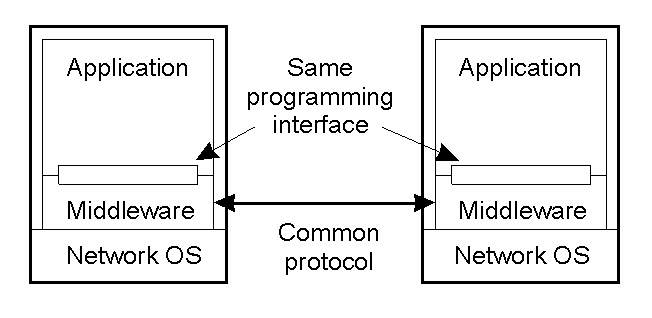
\includegraphics[width=1\textwidth]{pics/middlewareComm.jpg}
	\caption{Middleware based system \cite{Tanenbaum1}}             
	\label{fig:MddlewareComm}
\end{figure}  
%**********************
%**********************
\begin{figure}[!hbt]                               
	\centering                                           
	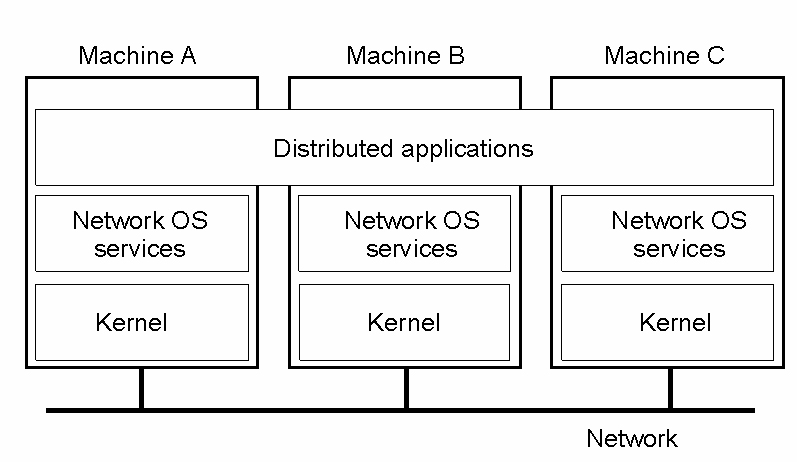
\includegraphics[width=1\textwidth]{pics/middlewareGeneral.jpg}
	\caption{Middleware based system \cite{Tanenbaum1}}             
	\label{fig:MiddlewareGeneral}
\end{figure}  
%**********************
Taking a look from the top, from the users point of view, the user will get a homogeneous view of the system. Using the applications and developing them you won't have to take care about the underlying heterogeneity. It provides a single and coherent view to its users. 
\\\\
A good example for better understanding is provided by \cite{Tanenbaum1}: 
\\\\
Orders are placed from different types of clients like notebooks connected to the network, from the telephone network or cell phones. Those incoming orders are processed by a workflow system and the result is a new internal shipping order from the planning department and a billing order from the accounting. The users are not aware of where those forwarded orders physically came from. It appears that they are from a single central authority.
%**************************************************************************************
\subsection{Middleware Layer}
%**************************************************************************************
The rise of client/server application architecture where system components access remote infrastructure and functionality to accomplish their own tasks has led to the need to decouple communication parties to assure the need for scalability in the current IT infrastructure. What makes this possible is the additional middleware layer that helps to hide the heterogeneity of the underlying platforms and improves transparency. The DOS\footnote{Disk Operating System} is not intended to handle a collection of independent computers and a NOS\footnote{Network OS services} does not provide a  view of a single coherent system. There are several models/paradigms describing the middleware layer:
\begin{itemize}
	\item Plan 9 was the first approach which treats everything as a file. The cause of this is because that it can be shared by several processes in the unix world and the communication is reduced to accessing files.
	\item Remote Procedure Calls (RPCs) allows to call functions and pass parameters on a remote machine. The callee does not know necessarily anything about the location of the remote function which can be on a machine physically somewhere else on the world.
	\item Distributed objects describes the method to invoke objects in a transparent way on remote machines by providing interfaces of those objects.
	\item The message oriented paradigm takes care about providing the same communication facilities so that systems can talk to each other. The content of the information itself is ignored by these type of middleware models.
\end{itemize}
%**************************************************************************************
\subsection{Communication Paradigms}
%**************************************************************************************
There are different communication paradigms we have to be aware of, before continuing:
\begin{itemize}
	\item \textbf{Transient communication} stores a message only as long as the sender and receiver is up and running.  
	\item \textbf{Persistent communication} on the other hand stores a message as long as the receiver retrieves it.
	\item \textbf{Asynchronous communication's} characteristic is that it sends a message and doesn't wait for a notification so it can keep on working without a halt.
	\item Applying \textbf{Synchronous communication} will result in a delay for the sender until a received notification will come in from the receiver. 
	\item \textbf{Broadcast} means that a sender is communicating to multiple receivers.
	\item \textbf{Point to Point} communication is simply that one communication link has been established between sender and receiver.
\end{itemize}

Today the message oriented middleware paradigm has become one of the communication pillars of today's enterprise systems. It is the most common communication facility for exchanging information. There are different ways of organizing message oriented middlewares, but the most important is the message queuing type. 
\\\\
\textit{Message-queuing systems provide extensive support for persistent asynchronous communication} \cite{Tanenbaum1}
\\\\
In practice each application has got it's own message queue or several applications share one queue. This enables applications to communicate with eachother by inserting messages into specific queues using message-queuing systems. This allows a loosely-coupled communication between systems. The inserted messages are pending in the queue as long as the receiver fetches it from the queue. So neither the sender or the receiver client has to be online if a message has been deployed in a queue. An important fact is that usually message-queuing systems don't guarantee the delivery of the sent messages. However there are mechanisms available in a variety of products to ensure the success of message transactions. This message based style communication bears the potential to integrate new autonomous, heterogeneous components into complex systems that are easy to evolve and scale \cite{LudgerFiege05}.
\\\\
As messages can contain any form of data the integration into a distributed system can lead to problems as applications provide different data formats. Message Brokers are an important component to act as a gateway between message-queuing systems. It transforms messages into a format that can be read by the different communication partners.
\\\\
The layering according to \cite{Tanenbaum1} is a very simple point of view as he only wants to show how a middleware can enable a transparent and single coherent view of a system. David Luckham introduces a slightly deeper granularity of the high level overview of a distributed, event-driven system in order to be able to understand the importance of events for enterprises.
\\\\
\textit{Layered IT systems present another dimension in the search for new ways to understand the events that happen in them.} \cite{Luckham05}
%**********************
\begin{figure} [h]                        
	\centering                                           
	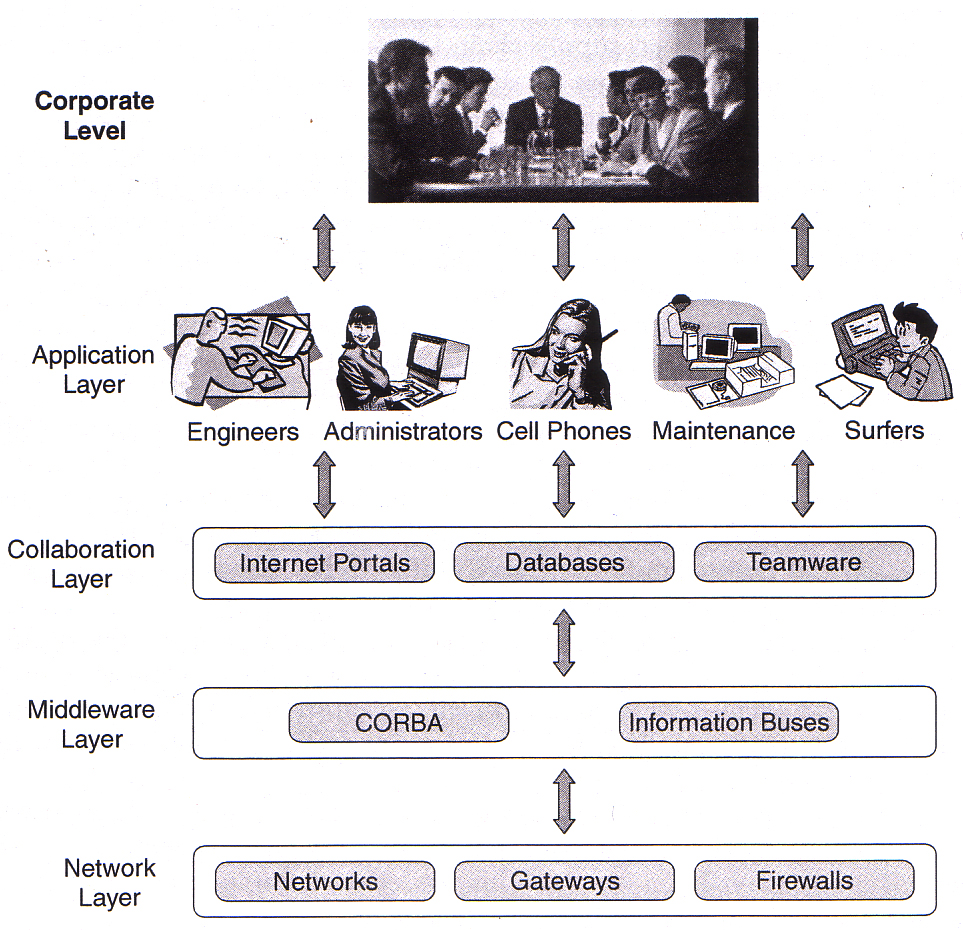
\includegraphics[width=1\textwidth]{pics/corporateLayer.jpg}
	\caption{Enterprise System Layering \cite{Luckham05}}             
	\label{fig:EnterpriseSystemLayer}
\end{figure}  
%**********************
\begin{itemize}
	\item \textbf{Corporate Level:} At this layer enterprises plan and transact their business. Applications like accounting, inventory, spreadsheets, e-mail clients, calendars, webbrowsers and in general, interfaces to other services, belong in here. It can be argued where services like email belong. Actually they would fit in the Application Layer as well.
	\item \textbf{Application Layer:} At this layer, events are generated on a high level by the user where they signify activities like sending an e-mail. Actually many events generated at this layer are not simply one event rather they are aggregated to a high level event from the events generated by the layers underneath.
	\item \textbf{Collaboration Layer:} This layer provides the basic infrastructure for applications like databases, e-mail servers, web servers and so on. The line between the application layer and the collaboration layer can be blurry.
	\item \textbf{Middleware Layer:} As mentioned above this is a very important part because it lets enterprise systems talk to each other.
	\item \textbf{Network Layer:} This layer is the basic layer where everything builds on top of it. At this layer only low level events are generated to transport information from A to B.
\end{itemize}

%**************************************************************************************
\subsection{On Events}
%**************************************************************************************
As we talk quite a lot about passing messages back and forth in enterprise systems what is the definition of an \textit{event} exactly? 
\\\\
In context of computer science an event is used to control the flow of a program. A well known application are user interfaces where triggered user interface elements generate events to start processes.
\\\\
According to \cite{Luckham05} an event is defined as:
\\\\
\textit{An event is an object that is a record of an activity in a system. The event signifies the activity. An event may be related to other events.} \cite{Luckham05}
\\\\
Ludger Fiege describes an event in his thesis as:
\\\\
\textit{Any happening of interest that can be observed from within a computer is considered an event}\cite{LudgerFiege05}
\\\\
For better understanding we follow \cite{Lamport78} and assume that we have a distributed system holding processes for receiving and sending messages. The dot represents occurred events and the dotted line represents a message. The vertical direction represents the time and the horizontal the space dimension.
\\\\
%**********************
\begin{figure}                         
	\centering                                           
	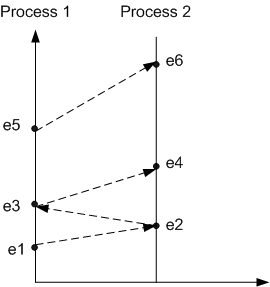
\includegraphics[width=0.6\textwidth]{pics/lamportEvent.jpg}
	\caption{Events and Messages}             
	\label{fig:LamportEvent}
\end{figure}  
%**********************
There are three aspects an event covers \cite{Luckham05}:
\begin{itemize}
	\item \textit{\textbf{Form:} An event is an object containing attributes or data components.}
	\item \textit{\textbf{Significance:} An event signifies an activity}
	\item \textit{\textbf{Relativity:} An activity is related to other activities by time, causality and aggregation.}
\end{itemize}
Furthermore an event usually contains an unique id and a timestamp to mark the creation of that event. 
\\\\
An example for events used in our system as a simulation model would be an OrderReceived event that signifies the activity of a posted order for some products \ref{lst:OrderReceivedEvent}:
\\\\
\begin{lstlisting}[caption=OrderReceivedEvent, label=lst:OrderReceivedEvent]{OrderReceivedEvent}
<OrderReceived>
	<OrderId>14765</OrderId>
	<DateTime>2005-10-31T11:31:02</DateTime>
	<DeliveryDate>2005-11-12T06:00:00</DeliveryDate>
	<Destination>Madrid</Destination>
	<ProductCollection>
		<Product>		
			<ProductId>Arzeutic</ProductId>
			<Amount>700</Amount>
		</Product>	
	</ProductCollection>
</OrderReceived>
\end{lstlisting}

Events are generated from different sources and different types. Normally they use some standard like the XML format. The received events must be transformed into a higher level form in order to be able to work with them. This transformation is provided by adapter components.
%**************************************************************************************
\subsubsection{Relationships}
%**************************************************************************************
According to \cite{Luckham05} there are three important relationships between events:
\begin{itemize}
	\item \textbf{Time:} Relates events according to their temporal occurrence
	\item \textbf{Cause:} Relates events according to their causal relationships. A causal relationship is given when an event A caused another event B in a direct or indirect way.
	\item \textbf{Aggregation:} Aggregates event to high level events based upon different criteria like time, causality or content patterns.
\end{itemize}
Following Luckham's \cite{Luckham05} proposal that a timestamp defines the time relationship between events is not as easy as he says that you can determine by the time dimension that \textit{event A happened before event B}. Leslie Lamport addresses this problem \cite{Lamport78}:
\\\\
\textit{In a distributed system, it is sometimes impossible to say that one of two events occurred first. The relationship ``happened before'' is therefore only a partial ordering of the events in the system.} \cite{Lamport78}
\\\\
The happens-before relation "$\rightarrow$" can be defined for following situations:
\begin{itemize}
	\item If a and b are events in the same process, and a comes before b, then a $\rightarrow$ b.
	\item If a is an event sending a message from one process and b is an event receiving the message from another process then a $\rightarrow$ b.
	\item The happens-before relation "$\rightarrow$" is transitive: a $\rightarrow$ b and b $\rightarrow$ c then a $\rightarrow$ c. 
	\item If two events, a and b, are distinct, they are called concurrent which means that you can't say which event happened first. In other words it means that if the events a and b happen in different processes and they do not exchange messages, then a $\not\rightarrow$ b and b $\not\rightarrow$ a.
\end{itemize}
%**********************
\begin{figure} [!h]                
	\centering                                           
	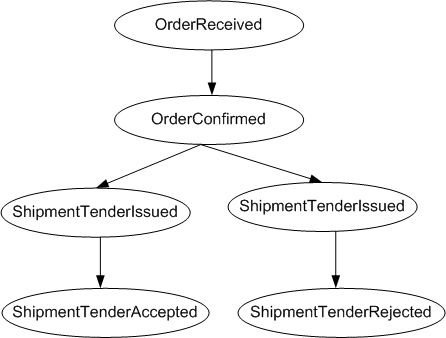
\includegraphics[width=0.7\textwidth]{pics/acyclicEventGraph.jpg}
	\caption{Directed acyclic graph of an event history}             
	\label{fig:dag}
\end{figure}  
%**********************
Martin Fowler is addressing another important issue regarding timing \cite{MartinFowlerTime}. Date and Time information can come in different  precision formats. You could get a date on a daily precision and you could get it on msec precision level depending on your application. But as you work with events collected from different sources this could become a problem especially in distributed environments over the Internet where different time zones come in too. Furthermore the question arises which event processes is counted? The one where the event happened physically on a machine or when it has been processed somewhere else? This kind of questions have to be considered when building a system to process or collect events from different distributed sources.
\\\\ 
In general a \textbf{causal relationship} determines that an event A caused another event B. As we have seen in our layered enterprise according to \cite{Luckham05}, events flow through these layered environment triggered by the user or another system at the top level. They are consequently transformed into lower level events down to the bottom causing other events to fire. This event flow is called \textit{vertical causality} and tracks down how high level events beginning from the business level manifest in lower layers. This is important to understand how these events are decomposed the way down in order to be able to create meaningful aggregations out of the masses of low level events. On the other hand Luckham talks about \textit{horizontal causality} that tracks the causal relationships between events at the same level. Causal relationships are transitive and asymmetric and can be represented as directed acyclic graphs (Figure \ref{fig:dag}). 
\\\\
\textit{Recognizing or detecting a significant group of lower-level events from among all the enterprise event traffic, and creating a single event that summarizes in its data their significance, is called event \textbf{aggregation}.} \cite{Luckham05}
\\\\
Aggregating events is a difficult task as it needs a technology that can recognize patterns of events through different layers. But if such an aggregation facility is set up and running, it can be a powerful source of tracking down causalities between events.

%**************************************************************************************
\subsection{Eventbased Systems}
%**************************************************************************************
The term of event-based systems is used in many fields in an ambiguous and varying way. As we have described several messaging architecture types like the persistent, transient and asynchronous way to deliver messages to a client, there is a distinct line between simple message exchange and event-based systems. The exhaustive trend of using distributed system architecture to support highly automated data processing has led to the concept of client-server architecture that brought major drawbacks with it. A classic client-server architecture, where system components access remote functionality to accomplish their own tasks, is often a synchronous communication between the server and the client. That leads to tight coupling and affects the scalability of such architecture models. Several middleware extensions addressed this problem by allowing to use asynchronous messaging, in an either persistent or transient way, using the mentioned message queuing techniques. 
\\\\
In an event-based environment we have components communicating with eachother by sending and receiving event notifications. There are mainly two interacting components the \textit{consumer} and the \textit{producer}. The consumer is subscribing to certain notifications and the other component, the producer, is publishing notifications about various topics. A notification service dispatches the notifications from the producer to the subscribed consumer. This notification service makes it possible to create loosely coupled and scaleable infrastructure as none of the components have to know about eachother. The notification itself is created by observing special occurrences that are a point of interest. For instance this could be events triggered by various systems. The subscription of consumers is a list of certain notifications the consumers wants to receive by the notification services. The subscription mechanism could be just a filter function or a more sophisticated notification selection mechanism including metadata descriptions. A channel would represent such a bundle of notifications that a consumer could subscribe and a producer could select to distribute its notifications.
\\\\
%**********************
\begin{figure} [ht]                
	\centering                                           
	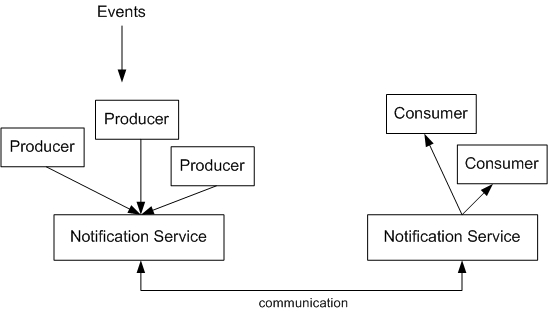
\includegraphics[width=1\textwidth]{pics/eventBasedConsumerProducer.jpg}
	\caption{Event-based notifications}             
	\label{fig:event-basedNotifications}
\end{figure}  
%**********************
\\\\
%**************************************************************************************
\subsection{Business Value}
%**************************************************************************************
As you can see there is the major drawback of missing filtering, aggregation and correlation services like mentioned in the introduction. Actually it is no big deal to set up a message queue for a component or a system to receive specific event notifications from a channel. Let's assume that you have a component or a system subscribed to a shipment tracking channel that sends continuous notifications about the current status of a package and another subscription to a channel that notifies about shipment audits. The system would be able to handle those received events according to its assigned tasks in ways like the following: 
\begin{itemize}
	\item \textit{The shipment xy has been audited and a damaged product has been identified.} The system can book product xy from shipment xy as damaged.
	\item \textit{The shipment xy has been delivered.} The system can book the shipment xy as finished.
	\item \textit{The shipment xy is currently on road between Vienna and Linz.} The system can react in sense that it updates some location tracking systems used.
\end{itemize}

There is a wide range of options how to deploy systems. It could be even done in ways that systems can react in very intelligent ways, but in sense of gathering high level business information or tracking business processes it won't be possible as you would need a facility that collects all events. It would even need access to historic data in some cases to find out for example what caused to failed the shipment from the example above. If you would like to create high level overviews of that shipment you need correlation information about those events that belong to one shipment or you would need aggregation functionality to create more abstract groupings of those information. Another problem dimension is that todays business environment requires a fast paced  decision infrastructure based on up-to-date information. For long people complied with that decision making does not require actual data instead it needs huge amounts of historical information collected in data warehouses. 
\\\\
\textit{[...] strategic decision makers are being exposed to the huge inflows of data and information from their resources and they are under rigid time constraints to make the right decisions.} \cite{NguyenSchieferTjoa05}
\\\\
According to Hackathrone the business value of taking an action goes down after an event happend (see Figure \ref{fig:Eventbusinessvalue}).

%**********************
\begin{figure} [ht]                
	\centering                                           
	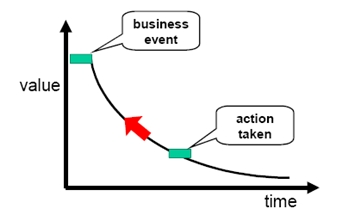
\includegraphics[width=0.8\textwidth]{pics/businessValue.jpg}
	\caption{Event business value \cite{Hackathorn02}}             
	\label{fig:Eventbusinessvalue}
\end{figure}  
%**********************
%**************************************************************************************
\subsection{Related Work to Eventbased Systems}
%**************************************************************************************
Currently there is quite a lot of work going on in the design and application of event-based system support and correlation systems. This section will introduce some of the most prevalent systems to get a feeling what is going on in this field and what types of approaches exist to handle the events.. Senactive's InTime\footnote{www.senactive.com} is undoubted the most relevant system for this diploma thesis as it delivers the simulation data. 

%**************************************************************************************
\subsubsection{Senactive InTime - Sense and Response Architecture}
%**************************************************************************************
%**********************
\begin{figure} [ht]                
	\centering                                           
	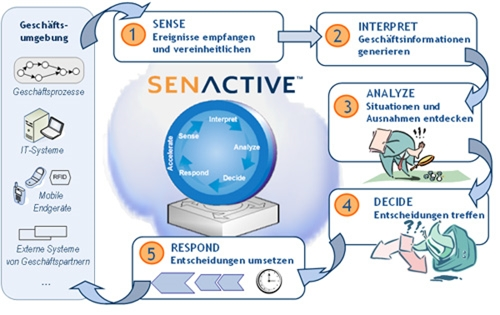
\includegraphics[width=1\textwidth]{pics/senseAndResponseSenactive.jpg}
	\caption{InTime Sense and Response Architecture \cite{SenactiveWebpage}}             
	\label{fig:senseAndResponseSenactive}
\end{figure}  
%**********************
The basic idea behind the \textit{Sense and Response Service Architecture} used in Senactive's InTime product is to monitor IT- and business processes in sense and response loops. This architecture allows to gather business intelligence data and make decisions based on actual information. Real-time event sources are connected to the system by event adapters and fed into \textit{Sense and Response loops} which is divided into 5 phases. 
\\\\
The 5 phases in detail (see Figure \ref{fig:senseAndResponseSenactive}) \cite{NguyenSchieferTjoa05} :

\begin{itemize}
	\item \textbf{Sense}: Continous capturing of events and unification by the sense and response architecture.
	\item \textbf{Interpret}: The events will be transformed into business information like performance indicators, business situations and exceptions.
	\item \textbf{Analyse}: Analysis of interpreted business information to predict performance and risks if the business environment changes.
	\item \textbf{Decide}: Proposal for the best business situation and the according actions to be done either automated or by involving humans.
	\item \textbf{Respond}: Communicating the decision made in the last step to change the business environment.
\end{itemize}

The processing, transformation and the relationship definition steps can be defined for every organization using an event processing model for modeling these sense and response loops.
\\\\
The system is capable of detecting exceptional business situations and can react on them by generating warnings or take measures by itself to prevent damages like fraud. The InTime product is also capable of correlating events and aggregating events from it's various sources. This product would help customers to monitor their event-driven enterprise systems from a high level perspective to gather financial ratios, to trace down occurred problems or to use it for decision making based on real time information. As this product can react proactively on given business situations in its \textit{decide cycle} it can change business situations autonomously based on rules and provided information. The change of business situations can be performed in an event-based manner again. 
\\\\
This \textit{Sense and Response Service Architecture} can be used to satisfy real-time business intelligence architecture requirements as it can be used as a real-time data cache that serves as a staging area for datawarehouse updates and analytical services. More on zero-latency data warehousing and real-time business intelligences has been addressed here \cite{TjoaNguyenKickinger04}, \cite{NguyenSchieferTjoa05} and \cite{ThoManhNguyen05}.
\\\\
A useful feature of Senactives InTime is an event simulator that can generate events to create simulations to test event workflows or to generate event-based data for other purposes. This feature has been used for this diploma thesis to simulate logistics service provider based upon some special exceptional stories created. 

%**************************************************************************************
\subsubsection{RAPIDE}
%**************************************************************************************
RAPIDE is an event pattern language developed at Stanford University by the Program Analysis and Verification Group under the lead of David Luckham. RAPIDE is a declarative computer language that enables the specification of patterns of events. The syntax of of RAPIDE is basically like today's languages like Java or C\#. RAPIDE allows the specification of patterns that form relationships between events by causal, content or temporal constraints. This language has the feature to add pattern rules during runtime while events are collected according to the given pattern rules and processed by given action statements. Rapide is capable of aggregating high level events out of a collection of correlated events.
\\\\
It has a rich set of features \cite{Luckham05} like:

\begin{itemize}
	\item Definition of Event types.
	\item Event pattern definition
	\item Pattern operators for modeling relationships between events.
	\item Temporal operators to specify the timing of events.
	\item Pattern macros for building more complex patterns.
\end{itemize}

According to \cite{LuckhamManensPark} RAPIDE is a good approach to test and simulate business process as it is easily possible to track causal relationships and to detect contraint violations during simulation. 

%**************************************************************************************
\subsubsection{Generalized Event Monitor - GEM}
%**************************************************************************************
%**********************
\begin{figure} [ht]                
	\centering                                           
	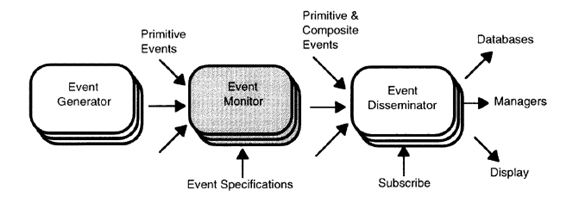
\includegraphics[width=1\textwidth]{pics/GEM.jpg}
	\caption{Event monitoring components \cite{GEM95}}             
	\label{fig:gemEventMonitoringComponents}
\end{figure}  
%**********************
The Generalized Event Monitor (GEM) is an interpreted declarative rule-based event monitoring language which allows to specify high-level events out of different nodes in a distributed system. The purpose of GEM is to monitor operations of distributed systems to support management decisions and control network behaviour. The monitor is capable of applying filters and to correlate events according to predefined rules. GEM's specification contains the type of the events to be collected, a pattern that has to be matched and an action to be performed. GEMs specification is very powerful as it allows the definition of triples (format, composite event definition and actions to be defined). Moreover it is possible to modify the GEM monitors state. The main drawback is that it does not support the modelling of causal relationships between events which result in a lack of defining patterns based on causalities between events. For further details see \cite{GEM95}.
%**************************************************************************************
\subsubsection{HP-ECS Event correlation service}
%**************************************************************************************
%**********************
\begin{figure} [ht]                
	\centering                                           
	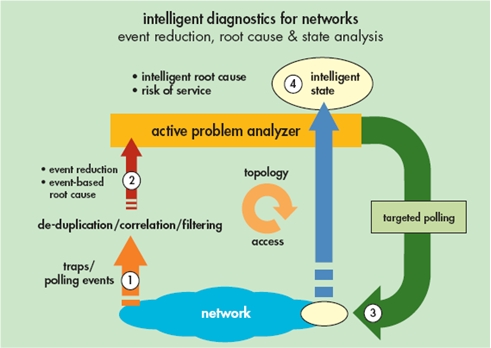
\includegraphics[width=1\textwidth]{pics/openView.jpg}
	\caption{HP-ECS OpenView \cite{OpenViewHP}}             
	\label{fig:openViewHPECS}
\end{figure}  
%**********************
Hewlett Packard provides a commerical event correlation product for correlating events coming from various system levels like the lower network layers, enterprise systems and application or database systems. HP-ECS correlates events by defining correlation circuits with a sophisticated GUI. These correlation circuits are a set of nodes connected to each other where the events pass through.  
\\\\
Events can be passed through intermediate nodes in a circuit that provides different features like:
\begin{itemize}
	\item temporal filters
	\item causal filters
	\item content filters
	\item in general event monitoring
	\item sequential event constructs 
\end{itemize}

HP-ECS has a major flaw because it is not usable for generic event correlation as it only supports correlation for SNMP\footnote{Simple Network Management Protocol} and CMIP\footnote{Common Management Information Protocol } events.

%**************************************************************************************
\newpage
\section{Scope of this diploma thesis}
%**************************************************************************************

We have seen in the previous chapters the impact events have in today's decision making processes and what value they create for process management, especially in large and global oriented enterprises. E-Business and E-Markets have created a global playground for automated workflow systems which result in a huge traffic flow of information between corporate networks and department systems. The lack of monitoring these events in a sense of correlating them, creating causal relationships or aggregate them to high level events is still a problem that is currently challenged by academic and commercial oriented institutions. Some of them, like Senactive's Sense and Response Architecture, provide the ability to monitor event flows and proactively react on them to change the business processes, based on real-time information, provided by the various enterprise systems. This is a major step towards real-time enabled enterprises that can challenge the requirements of today's highly dynamic business world. 
\\\\
The core of this diploma thesis does not go into event-based processing problems like creating sophisticated causal trackings or correlation algorithms in first place. This thesis is about a system that enables the historic view of collected historic event streams that have been preprocessed by Senactives InTime Sense and Response Architecture. As Intime can react proactively on given business situations based on event constellations and defined rules, it can rearrange business processes to stear the business environment and processes into a given direction. This will result in a chain of newly triggered event flows which join back to the control loop. InTime is capable of correlating events according to predefined rules and delivers causal tracking of events. 
\\\\
The system developed in this diploma thesis is collecting those \textit{catched} events and creates a full text index over them to enable a Google like search experience for investigation purposes. The major application of this system is to offer the user a toolset to discover different aspects of business processes based on event correlations. This system has evolved over several stages to clarify which architecture would be the best solution to provide this kind of search and discovery experience to a user and at the same time to lay the foundation for further work in the area of event mining and correlation discovery. 

%**************************************************************************************
\newpage
\section{Information Findability}
%**************************************************************************************
According to \cite{Morville05} findability is described by following aspects:

\begin{itemize}
	\item \textit{The quality of being locatable or navigable.}
	\item \textit{The degree to which a particular object is easy to discover or locate.}
	\item \textit{The degree to which a system or environment supports navigation and retrieval.}
\end{itemize}

Google has shown the world that searching the web does not have to be based on simple keyword matchings or word frequency countings. It introduced a completely new way of rating webpage contents and to calculate the best hits out of some search terms, provided by the user. Google's commercial success has proven that this way of finding information is the right one, at least for the moment as long as noone else comes with a better idea. 
\\\\
The look and feel of Google's way finding and retrieving information has become a defacto standard. Numerous applications integrate full text indexing algorithms and methods into their applications to provide a search based access to information and data. These applications don't necessarily concentrate on finding webpages. The search can be applied on a variety of information like office documents, products, flight schedules or even free available source code. People tend to move away from the classic topologic of classifying information into tree like catalogues and let the user navigate through these structures to get his desired information. A good indexing and retrieval mechanism allows the user to find and access information by typing some terms into a textbox and a ranking algorithm calculates the best hits out of the found information to present the most relevant information. This way of organizing the access to information has become a great success as numerous applications has proven like koders.com, Google Desktop Search and Apple's Spotlight for instance. 
\\\\
\textit{Of course, access doesn't simply require us to make decisions in more areas of our lives. It also changes the game by inviting us to make informed decisions more often.} \cite{Morville05}

%**************************************************************************************
\subsection{Event Cloud Background}
%**************************************************************************************

% welchen bedeutung hat event cloud? siehe scope
% was kann der Benutzer damit machen?
% Grundlage f�r Eventmining und correlation finding
% Geeignete Architektur f�r so eine Anwendung finden
% Fokus auf freie Technologien

Event Cloud is the name of the developed application whose main purpose is to provide a search interface to its users to allow them to search for simple and correlated events in an efficient way.  The representation of the search results is a major feature that allows its user to get the most relevant hits according to the given search criteria. Furthermore it provides functions to exclude unwanted event and correlation types from the found result set and it allows to create filters over events and their correlations. As not every person is interested in all types of occurred events and correlationsets it is possible to create and edit roles for different user profiles that will reduce the information pool to a desired manageable pool of events and correlations. Event Cloud provides the user the option to dig down to event levels or to go up to correlation levels according to the selection from a found resultset. 
\\\\
Basically, Event Cloud has implemented two Search types that allows a user to query for either events or to search through whole event correlations. Using the latest Java high-performance text search engine library Lucene and the powerful open source database Postgres allows to index and search the event repository in a fast and efficient way. The system is supported by the lightweight IoC\footnote{Inversion Of Control aka dependency injection} Spring framework to bind the components together. A special focus has been set on using only non-proprietary and Open Source technologies as this is an academic project and should lay the cornerstone for future work on this topic or at least provide useful information how to do or not to do future work in this field. 
\\\\
Event Cloud consists of three main functions: 

\begin{itemize}
	\item Extracting and transforming event data from the source system and integrate them into Event Cloud's own data structure.
	\item Full text index over simple and correlated events.
	\item Search functionality including a sophisticated query syntax and various filter functions.
\end{itemize}

These functionalities should provide a powerful toolset to facilitate the discovery of different aspects of business processes based on event correlations provided by a ``  ``Google-like'' search experience. 
\\\\
This diploma thesis was especially supported by Josef Schiefer and Senactive, by providing InTime for the basic infrastructure and support throughout the whole developing process. Especially the simulation of business processes to gather test data in form of generated events was done by the InTime product. Plenty of time has been invested to create interesting and meaningful simulations of business processes based on a logistics company. The event simulation has been broadened by according stories for showcases to display exceptional situations and to show how InTime can react on such situations. The simulation definition process has been co-developed by Roland Vecera and is available as an Appendix in the diploma thesis to get a comprehensive view of what happens beneath the fact that events exists for this project.
\\\\
As we talk about source systems or the source database throughout the next sections it is always the InTime database meant. This is a MS SQL Server database that contains the raw event information from the InTime simulator. As InTime is settled in the .Net world, Event Cloud provides an import functionality to duplicate the database on a desired machine, because InTime has been deployed in a VMWare for developing purposes which is not a performance wonder.

%**************************************************************************************
\newpage
\subsection{Search Concepts}
%**************************************************************************************
% Das Suchen ist der zentrale Teil daher muss man bestimmte Suchkonzepte unterscheiden die
% vom System unterst�tzt werden.
The subsequent chapters will give a conceptual overview of the search type features provided by Event Cloud. These are the basic concepts behind the Event Cloud and no further technical details are provided in this section.

%**************************************************************************************
\subsubsection{Rank 1}
%**************************************************************************************
The Rank 1 search is a simple full text search over all searchable attributes of an event. The user is able to put down a search query consisting of several search terms and boolean operators according to Lucenes BNF query syntax. The result will be a list of events that matched the given query. 
\\\\
The Rank 1 search is pretty straight forward like you would search documents on the internet using any search engine available. 
\\\\
Take a look at the example (Figure \ref{fig:rank1searchExample}) where we have several events in our repository. The user queries for the terms ``Paris London Szabolcs'' and gets back the events TransportEnd and TransportStart as these terms occurred in those events ordered by the most relevant hits. No boolean operators have been applied in this query example. If the user would have entered a query like ``szabolcs AND Paris'' he would have received events where the terms Paris and Szabolcs would have occurred. For more details take a look at the query syntax as this is not in the scope of this chapter.
%***********************
\begin{figure}[ht]                                  
	\centering                                           
	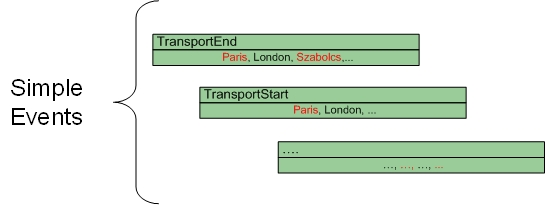
\includegraphics[width=1.0\textwidth]{pics/rankOneSearchExample.jpg}
	\caption{Rank 1 search example}             
	\label{fig:rank1searchExample}
\end{figure}            
%***********************      
%**************************************************************************************
\subsubsection{Rank 2}
%**************************************************************************************
At the current point the heart of Event Cloud is the Rank 2 search which is an extension of the Rank 1 search. The difference between Rank 1 and Rank 2 search is that this search type is not looking at events at an atomic level rather it searches over whole correlations of events (Figure \ref{fig:rank2correlation}). By executing a Rank 2 search the query will go over whole correlationsets of events instead of looking only at events like in the Rank 1 search type. 
\\\\
%***********************
\begin{figure}[h]                                  
	\centering                                           
	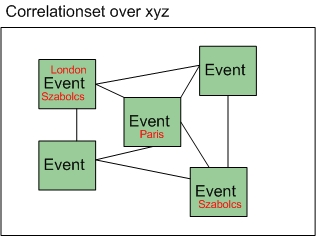
\includegraphics[width=0.7\textwidth]{pics/rankTwoSearchExample.jpg}
	\caption{Rank 2 search example}             
	\label{fig:rank2searchExample}
\end{figure}            
%***********************   
If a user puts down a search query consisting of terms like ``Paris London Szabolcs'' the search engine will retrieve correlations consisting of events that matched these terms (Figure \ref{fig:rank2searchExample}). That means that you will get back a correlation whose event attributes contain either Paris, London or Szabolcs. Correlationsets whose Events would not contain the terms ``Paris London Szabolcs'' would not be considered. If for instance a correlationset is consisting of eight events and only one event contains the search terms it would be still a hit but maybe a bad one depending on the other found hits.
%***********************
\begin{figure}[h]                                  
	\centering                                           
	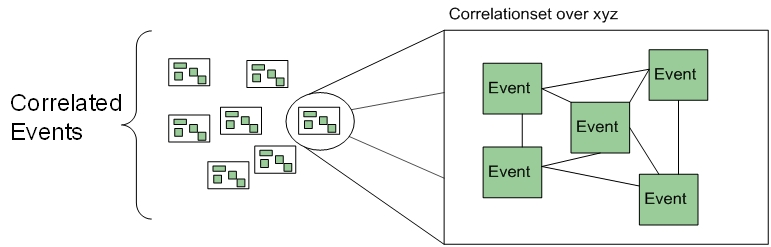
\includegraphics[width=1.0\textwidth]{pics/rankTwoCorrelation.jpg}
	\caption{Event correlation}             
	\label{fig:rank2correlation}
\end{figure}            
%*********************** 
   
%**************************************************************************************
\subsubsection{Rank 3}
%**************************************************************************************
This type of search is not implemented in the current work as it is a very complex topic and beyond the scope of this diploma thesis. For the sake of completeness I want to give a brief overview about this event search type. 
\\\\
The Rank 3 is searching over correlations like the Rank 2 search, but instead of using direct correlations between events it searches over indirect correlations between correlationsets. It is actually the same like the Rank 2 but one aggregation level higher and the result hits are additionally evaluated by a distance factor of these indirect correlations.
\\\\
The challenge behind this type of correlation search is to discover indirect correlations between events and to implement an effective search algorithm to rank the most relevant hits. This technique could become a performance eating task as you have to find a way to consider a higher aggregation level when querying for events.
%***********************
\begin{figure}[h]                                  
	\centering                                           
	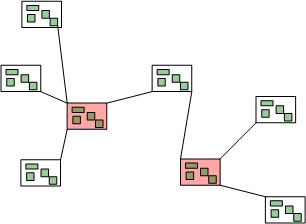
\includegraphics[width=0.5\textwidth]{pics/rankThreeSearchExample.jpg}
	\caption{Rank 3 search}             
	\label{fig:rank3searchExample}
\end{figure}            
%***********************  
%**************************************************************************************
\newpage
\section{Architecture}
%**************************************************************************************
% Hier fangen jetzt die Details an! High level Architektur + Technologien genau beschreiben
% High Level overview mit Bild und kurz die Komponenten beschreiben und wie sie zusammenspielen
% simulator f�r eventsimulation kurz erw�hnen und details dann beim Simulator abschnitt selber schreiben.
Event Cloud is a webbased application based on the lightweight Spring Framework IoC container and is deployed inside Apache's Tomcat. The core technologies for O/R Mapping and Indexing/Searching are Hibernate and Apache Lucene (Figure \ref{fig:eventCloudHighLevel}). 

%**************************************************************************************
\begin{landscape}
%\subsubsection{High level overview}
%**************************************************************************************
%***********************
\begin{figure}[ht]                                  
	\centering                                           
	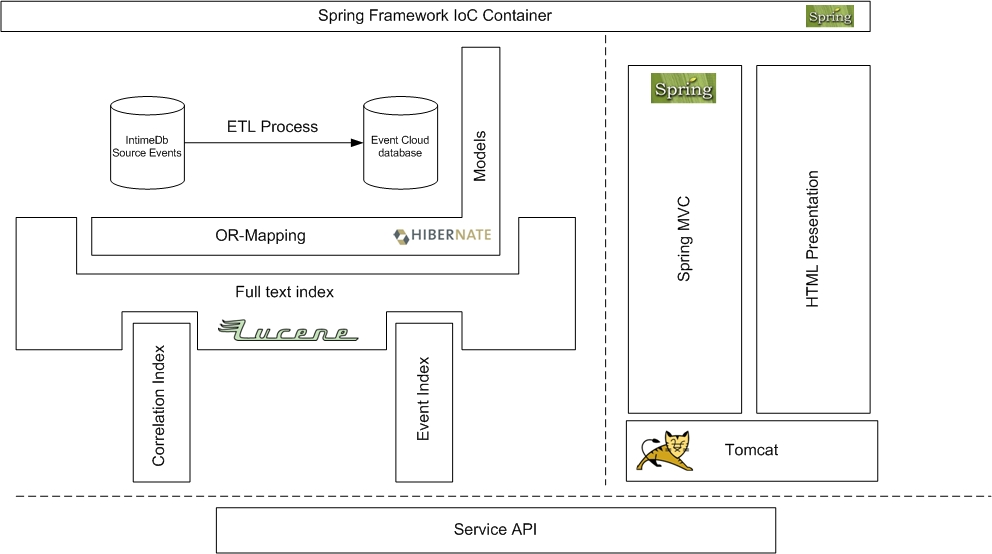
\includegraphics[width=1.2\textwidth]{pics/EventCloudHighLevelOverview.jpg}
	\caption{Event Cloud High Level Overview}             
	\label{fig:eventCloudHighLevel}
\end{figure}            
%***********************                       
\end{landscape}

%**************************************************************************************
\subsection{Database and Schemas}
%**************************************************************************************
There are two databases used by this system. The first one is the source database provided by InTime which contains the raw source events and the found correlationsets for those events. This is a Ms SQL Server database that requires the sqljdbc drivers in order to establish a connection from hibernate. As the second database there is currently a Postgres 8.1 database in use as it is open source and a powerful technology that fits the needs for this project. However using Hibernate as the O/R mapping facility it is possible to change the database backend with only minor changes. Only sequence definition changes have to be done at the mapping level as Postgres is using sequence tables for id generation. The source schemas are pretty straight forward flat tables (Figure \ref{fig:intimeschema}) and the final target schema created out of the source events is bit more complex as Event Cloud decomposes the events and stores them into a relational form (Figure \ref{fig:eventCloudSchema}). 
\\\\
%***********************
\begin{figure}[h]                                  
	\centering                                           
	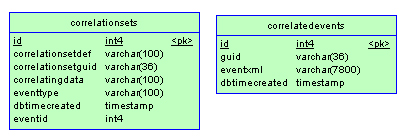
\includegraphics[width=1.0\textwidth]{pics/intimedb.jpg}
	\caption{InTime schema}             
	\label{fig:intimeschema}
\end{figure}            
%***********************
The rwtime and txtime tables represent the realworld dates of events (rwtime) e.g. when they really occurred in some system.  The timepoint when events have been recognized by the system are decomposed and stored in the txtime table. During the ETL process the event timestamps are decomposed to a day, month and year granularity. The rwtime and the txtime tables hold every possible combination of day, month and year as the event numbers grow and only the ids are assigned to the event. This allows an efficient indexing of the dates and thus a fast way to create constrained date queries.
\\\\
The events and eventattributes relations \ref{fig:eventCloudSchema}are the core tables in the target schema of Event Cloud. Basically the event relation holds the core event information provided by each event. The eventattributes relation holds every extracted attribute from an event, its value and its unique URI as events are constructed out of XMLs that can contain a complex structure. The logical XML structure is flattened in the relational form to preserve the original substructures a URI is saved to the database. 
\\\\
Consider for example the mentioned OrderReceived Event (Listing \ref{lst:OrderReceivedEvent}) where you have got basic information provided with a Productcollection containing a subtree of several products. 
\\\\
A representation in the eventattributes relation would look like provided in Figure \ref{fig:OrderReceivedInEventattributes}.
%***********************
\begin{figure}[h]                                  
	\centering                                           
	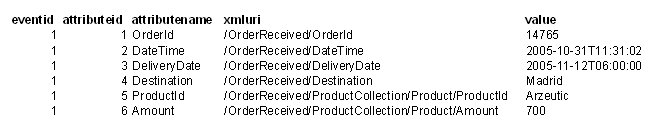
\includegraphics[width=1.2\textwidth]{pics/OrderReceivedInEventattributes.jpg}
	\caption{OrderReceived in eventattributes}             
	\label{fig:OrderReceivedInEventattributes}
\end{figure}            
%***********************  

The relation dbinfo is used to save information about the loading process and profiles is needed to store profile information about filters for the search functionality.
\\\\
The Index functionality of Postgres is a vital function that has been applied to the Event Cloud schema in Postgres to boost up performance. The standard index type of Postgres is a btree index which fits the needs as it can handle equality and range queries. Once the index has been created it will be updated automatically, but VACUUM ANALYSE has to be executed in regular intervals to update statistical data for the query planner. This has to be done especially when big amounts of data have been inserted into the database. Regular analysis can be executed by creating cron jobs over night for instance. 
\\\\
VACUUMing is important as rows are not physically deleted by Postgres, if they are removed, so this is necessary to reclaim storage space. VACUUming can be performed while reading and writing to tables as no lock is obtained but it will need some performance while running. 
\\\\
At this point it should be mentioned that Postgres is capable of handling different sorts of indexes found in \cite{PostgresDoc06} like partial indexing which could be useful to index only a subset of data stored in a table. This can be done by creating an index with a WHERE clause to specify the desired dataset. 
\\\\
Event Clouds indexes are set on relation attributes according to Table \ref{tab:indexedAttributes}.

\begin{table} [h]
	\begin{tabular}{ll}
	 \textbf{Tablename} &  \textbf{Attribute} \\
	
	   	dbinfos &         id \\
	
		eventattributes & attributename \\
		
		eventattributes &    eventid \\
		
		eventattributes &      value \\
	
	 	eventtype & eventtypeid \\
	
	    rwtime &      rwday \\
	
	    rwtime &    rwmonth \\
	
	    rwtime &     rwyear \\
	
	    txtime &      txday \\
	
	    txtime &    txmonth \\
	
	    txtime &     txyear \\
	\end{tabular}  
	\caption{Indexed Attributes}
	\label{tab:indexedAttributes}
\end{table} 
     
%***********************
\begin{figure}[h]                                  
	\centering                                           
	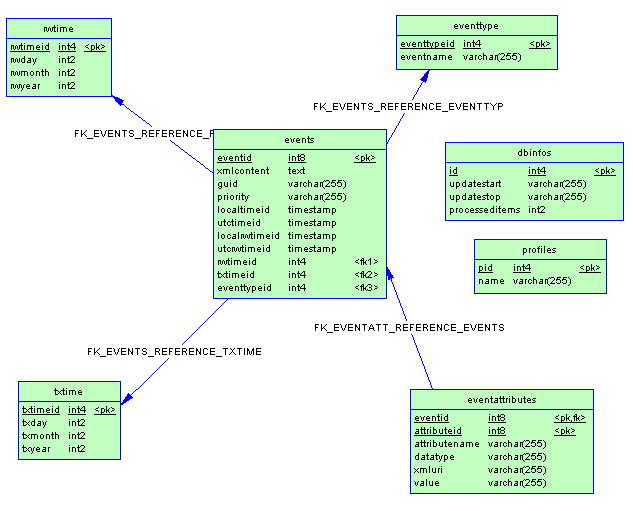
\includegraphics[width=1.0\textwidth]{pics/genericdb.jpg}
	\caption{Event Cloud schema}             
	\label{fig:eventCloudSchema}
\end{figure}            
%***********************     


%**************************************************************************************
\subsection{Object Relational Mapping}
%**************************************************************************************
We have seen in the previous chapter that the event sources and the transformed events are stored into relational databases. The whole data structure is based on a relational modeling paradigm which has proven itself over many years. The relational database technology has been originally introduces by E. Codd out of growing needs to structure data under specific standpoints and his works influence is still noticeable. Almost every application needs a way to make its data persistent after shut down, so a variety of products emerged over the years to provide a persistent and structured way to store application data.
\\\\
Codd firstly introduced the relational model in his paper ``A Relational Model of Data for Large Shared Data Banks'': 
\\\\
\textit{It provides a means of describing data with its natural structure only--that is, without superimposing any additional structure for machine representation purpose. Accordingly, it provides a basis for a high level data language which will yield maximal independence between programs on the one hand and machine representation on the other.} \cite{Codd70} 
\\\\
A relational database is mainly characterized by of following terms \cite{Codd99}:
\begin{itemize}
	\item data independence from hardware and storage implementation
	\item automatic navigation
	\item nonprocedural language for accessing data
\end{itemize}

This had a big impact and changed the way how data has been processed. Instead of manipulating record by record it was possible to describe the datasets for processing and to store data in an efficient way. Today a database management system is more than a formal description of how to organise and structure information. It provides a full blown information management system that allows applications to access large amounts of data in a fast manor. It supports transactions, user management, issues security topics and much more. Moreover the relational world has been and is still under academic discussions which helps to evolve the algorithms and technologies powering those technologies. A lot of work has been invested to mathematically formalize relational model and to develop a structured query language. Currently there is a wide range of commercial and open source database management systems available like DB2, Orcale, Ms SQL Server, MySQL or PostgreSQL.
\\\\
As time goes by people realized that procedural programing paradigms create too much overhead that makes systems difficult to maintain, components hard to reuse and the world could be described in better ways for problem solving. As a result the object oriented paradigm has evolved and Smalltalk was the first noticeable programming language that introduced the object oriented programming paradigm together with cutting edge features (at least for that time). During the mid eighties C++ established the object oriented paradigm into everybodies minds. Programming languages evolved over time and today's most widely spread languages are C++, Java and .Net derivates. Especially Java has proven itself for developing distributed applications. Today we have a sophisticated toolset available like modelling languages such as UML or a rich set of design patterns for different purposes we can use more or less out of the box (for more details take a look at \cite{DesignPatterns97} and \cite{Fowler97}).
\\\\
Today we are facing the problem of a \textit{paradigm mismatch}. We started to use object oriented techniques to model and develop our applications, but almost all of our  systems have the requirement that they need to persist their data. Following the object oriented paradigm we create domain models about the subjects we need to work with. Sometimes these models are named business models in a layered application context. This object oriented style of modeling our data clashes with the well known relational \textit{row and column world}. The problem is that object oriented domain models are simply the better choice as they help to improve code reuseability and the maintainability significantly. 
\\\\
The first approaches that addressed this problem were to create sql support to enable a link between the relations stored in a database and the business models to benefit from their advantages. This approach is very expensive as the developers have to write low level SQL statements using database APIs into the source code directly not to speak about the almost unchallengeable task to implement sophisticated algorithms like lazy-loading of object graphs that represent 1:n relations in a relation model or caching techniques to improve performance. You never would have thought about changing the database at the back end of such an implementation and even a schema change can get out of hand. Developers face huge problems that don't belong to the given business domain problem at all in order to create a clean and object oriented application.
\\\\
The solution to this problems is the object relational mapping (ORM) approach that keeps the developers away from the underlying persistence mechanisms. Developers only need to create a persistence layer that declarativly wires the business models to their relational counterparts. The underlying persistence mechanism does the rest for the developer including sophisticated techniques to boost performance for instance.
\\\\
\textit{In a nutshell, object/relational mapping is the automated (and transparent) persistence of objects in a Java application to the tables in a relational database, using metadata that describes the mapping between the objects and the database. ORM, in essence, works by (reversibly) transforming data from one representation to another.} \cite{HibernateInAction05}
\\\\
The main features provided by ORM approach are:
\begin{itemize}
	\item It shields developers from low level sql coding.
	\item It let the developers concentrate on business problems.
	\item It reduces development time significantly.
	\item It produces less lines of code that makes understanding a system and refactoring easier.
	\item It is database independent.
\end{itemize}
There are several ORM libraries available. For this project the decision has been made to use Hibernate, because it is wide spread and meanwhile a rock solid Java library with a big support community. It was important to keep the database technology out of scope in this project. Although the decision has been made to use Postgres for Event Cloud we wanted to keep the option to deploy other database technologies. Another important fact is that Hibernate has an outstanding performance as it creates almost no overhead and is able to make use of sophisticated caching mechanisms.

%**************************************************************************************
\subsubsection{Data Access Object}
%**************************************************************************************

Event Cloud uses the Spring Framework to manage the components of this application by applying the Factory Pattern, IoC and code injection. More on this topic later on. What's important is to be aware of, that the Spring Framework is taking over a lot of work handling Hibernate and data access. Spring supports declarative definition of the Factory pattern and a dependency injection.
\\\\
The Spring Framework brings a Data Access Object (DAO) support with it that is applied in Event Cloud. The idea behind DAO is to follow object oriented principles and thus to program against interfaces. You define a DAO interface and a concrete implementation of this DAO. The application now can access the DAO interface through higher level services (Figure \ref{fig:DAOconcept}). Spring binds the DAO implementation to the interface. This enables a loosely coupled design, improves maintainability and speeds up testing processes. Moreover the DAO pattern has the advantage that is easily possible to change the underlying data access even much faster.
\\\\
%***********************
\begin{figure}[ht]                                  
	\centering                                           
	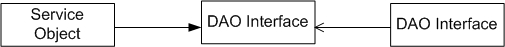
\includegraphics[width=1.0\textwidth]{pics/DAOConcept.jpg}
	\caption{DAO concept}             
	\label{fig:DAOconcept}
\end{figure}            
%*********************** 

%**************************************************************************************
\subsubsection{Integrating Data Access}
%**************************************************************************************

The Figure \ref{fig:SessionFactory} shows the basic wiring to establish database connections and integrate the data access into the application. The centerpiece of the data access, in Spring Framework managed applications, is the SessionFactory. The SessionFactory serves as a factory for dependency injections on thread safe DAOs. Event Cloud uses the LocalSessionFactoryBean as a concrete implementation which is appropriate for most types of scenarios even to deploy distributed transaction support or JNDI support. It is all just a matter of configuration. For example if we would want to change the database connection to a JNDI resource we just change the LocalSessionFactoryBean implementation to JndiObjectFactoryBean and readjust the connection string. 
\\\\
%***********************
\begin{figure}[h]                                  
	\centering                                           
	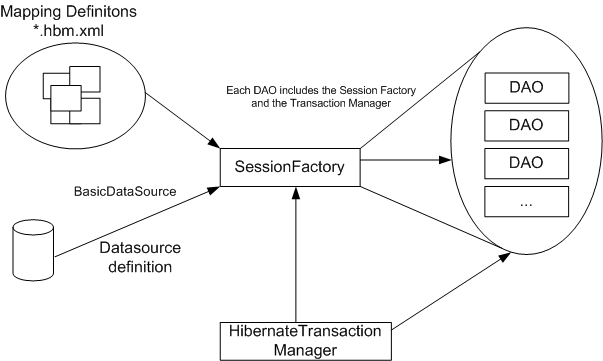
\includegraphics[width=1.0\textwidth]{pics/SessionFactory.jpg}
	\caption{Data Access integration}             
	\label{fig:SessionFactory}
\end{figure}            
%*********************** 
The listing figure \ref{lst:SessionFactoryConfiguration} shows a bunch of configuration options that have to be applied. Important to note is to specify the SQL dialect according to the database management system and create an injection link to you database connection bean (<ref bean="postgresSource"/>) which will be wired in by the Spring Framework. The hibernateProperties allow some fine tuning options like caching options and switches to turn on and off to help debugging.
\\\\
%***************************************
\begin{figure}[h]  
	\begin{mytinylisting}
	\begin{verbatim}
	<bean id="sessionFactoryForPostgresSource" class="org.springframework.orm.hibernate3.LocalSessionFactoryBean">   
		<property name="dataSource"><ref bean="postgresSource"/></property>
        <property name="mappingResources">
            <list>
            	<value>Event.hbm.xml</value>
				<value>Rwtime.hbm.xml</value>
				<value>Txtime.hbm.xml</value>
				<value>Eventattribute.hbm.xml</value>
				<value>Eventtype.hbm.xml</value>
				<value>Dbinfo.hbm.xml</value>				
            </list>
        </property>
        <property name="hibernateProperties">
        <props>
            <prop key="hibernate.dialect">org.hibernate.dialect.PostgreSQLDialect</prop>
            <prop key="hibernate.hbm2ddl.auto">update</prop> 
			<prop key="hibernate.show_sql">true</prop>
			<prop key="hibernate.cache.provider_class">org.hibernate.cache.EhCacheProvider</prop>
        </props>
        </property>
    </bean> 
   	\end{verbatim}
	\end{mytinylisting}
	\caption{The data access heart the SessionFactory configuration}             
	\label{lst:SessionFactoryConfiguration}
\end{figure} 
%***************************************
An important property is the mappingResource as it defines the mapping resources for the application. The mapping resource files are ending with a *.hbm.xml by standard and they provide the mapping definitions between the relational and the object oriented world. Creating and parameterizing the mapping resources is far out of scope in this diploma thesis as there is an excellent documentation available on the Hibernate webpage. Important is that there are tools and techniques available that can generate these mapping configuration files for your application. In this project a top-down approach has been chosen to create data access. The idea is to create the relational database schema and define various constraints. The next step is to apply a tool name Middlegen which is capable of reading in the database schema and provide a user interface to create the object relational mapping resources. When this has been done a tiny program can be integrated using Jakarta's Ant to generate the object oriented models including object graphs for representing relationships. Afterwards all that have to be done is add the mapping resource names to the SessionFactory.
\\\\
The database connections are defined in the context definitions of the application. One for the target database, the Event Cloud, and one for the source database (see listing figure \ref{lst:DatabaseConnection}). As we have two databases another SessionFactory instance for the second database has to be created too. For means of simplicity there is only one example provided just to show how the basic concept works if changes have to applied and how this is all wired together. Event Cloud makes use of the commons pooling package to provide basic connection pooling for the application. If someone would like to use a more sophisticated implementation like C3PO it is again just a matter of changing the class. 

%***************************************
\begin{figure}[h]  
	\begin{mytinylisting}
	\begin{verbatim}
	<bean id="postgresSource" class="org.apache.commons.dbcp.BasicDataSource">
	  <property name="driverClassName"><value>org.postgresql.Driver</value></property>
	  <property name="url"><value>jdbc:postgresql://localhost/generic</value></property>
	  <property name="username"><value>postgres</value></property>
	  <property name="password"><value>postgres</value></property>
	</bean>
	\end{verbatim}
	\end{mytinylisting}
	\caption{Database Connection}             
	\label{lst:DatabaseConnection}
\end{figure} 
%***************************************


%**************************************************************************************
\subsubsection{Transaction Management}
%**************************************************************************************

Now it comes an important topic: the transaction management. Spring Framework supports a wide range of transaction managers and the transaction management itself can be configured in a declarative way for each DAO and each method of the data access objects used in the application. Event Cloud makes use of the HibernateTransactionManager that is wired to the SessionFactory (Listing figure \ref{lst:Transactionmanagement}). Note that this is a huge step! For long declarative transaction management was only supported by EJB which had to be deployed inside heavy weight application servers with a wide range of drawbacks. The Spring Framework comes with declarative transaction support implemented through Spring's AOP framework. 
\\\\
%***************************************
\begin{figure}[h]  
	\begin{mytinylisting}
	\begin{verbatim}
	<bean id="transactionManagerForPostgresSource" class="org.springframework.orm.hibernate3.HibernateTransactionManager">
        <property name="sessionFactory">
        	<ref bean="sessionFactoryForPostgresSource"/>
        </property>
	</bean>
	\end{verbatim}
	\end{mytinylisting}
	\caption{Transaction management}             
	\label{lst:Transactionmanagement}
\end{figure} 
%***************************************

The DAO, created by the user, references the previously defined SessionFactory and has to extend the HibernateDaoSupport. The TransactionProxyFactoryBean is used to enable the declarative transaction management for a DAO. It needs three properties to be defined:

\begin{itemize}
	\item The transaction manager - in this case it is the HibernateTransactionManager
	\item The transaction target - this is a reference to the DAO that includes the SessionFactory
	\item The transaction attributes - declares which transaction type to apply to which methods including options.
\end{itemize}

%***************************************
\begin{figure}[h]  
	\begin{mytinylisting}
	\begin{verbatim}
	<bean id="correlatedEventDAOTarget" class="at.generic.dao.hibernate.CorrelatedeventDAOHibernate"> 
    	<property name="sessionFactory"> 
    		<ref bean="sessionFactoryForSQLServer"/> 
    	</property> 
    </bean>
	
	<bean id="correlatedEventDAO" class="org.springframework.transaction.interceptor.TransactionProxyFactoryBean"> 
    	<property name="transactionManager"> 
        	<ref bean="transactionManagerForSQLServerSource" /> 
      	</property> 
		<property name="target"> 
		   <ref bean="correlatedEventDAOTarget" /> 
		</property> 
      <property name="transactionAttributes"> 
         <props> 
            <prop key="save*">PROPAGATION_REQUIRED</prop>
            <prop key="update*">PROPAGATION_REQUIRED</prop> 
            <prop key="remove*">PROPAGATION_REQUIRED</prop>
			<prop key="*">PROPAGATION_REQUIRED, readOnly</prop>
         </props> 
      </property>
    </bean>
	\end{verbatim}
	\end{mytinylisting}
	\caption{Integrating transaction management for a DAO}             
	\label{lst:TransactionmanagementDAO}
\end{figure} 

The transaction attributes cover propagation rules and isolation levels that can be defined for each method. The key properties define on which methods they should be applied. For example on methods starting with ``save*'' Propagation is required (Figure \ref{lst:TransactionmanagementDAO}).
\\\\
A detailed explanation of the propagation rules is available here \cite{SpringInAction05}). Event Cloud mostly uses the PROPAGATION REQUIRED which will create a transaction for the methods. The read-only option is important to apply for attributes that perform only read operations as this option activates certain optimizations that may boost up the performance during such transactions. There are also five isolation levels available to set that are also described in detail here \cite{SpringInAction05}. 

%**************************************************************************************
\subsubsection{Event Clouds Persistence Layer}
%**************************************************************************************

Event Cloud's data access is following the data access object (DAO) pattern, using Hibernate and Spring Frameworks support, described in the previous sections. For each database there are models generated using a top-down approach. The resource mappings between the relational database and the business objects or models are generated by middlegen and out of these mappings codegen generates the models according to their relational structure. 
\\\\
There are 8 model classes available that represent Event Cloud's target schema:
\begin{itemize}
	\item Dbinfo
	\item Event
	\item Eventattribute
	\item Eventtype
	\item Filter
	\item Profile
	\item Rwtime
	\item Txtime
\end{itemize}

And there are two model classes that represent Event Cloud's source schema from InTime:
\begin{itemize}
	\item Correlatedevent
	\item Correlationset
\end{itemize}
%***********************
\begin{figure}[h]                                  
	\centering                                           
	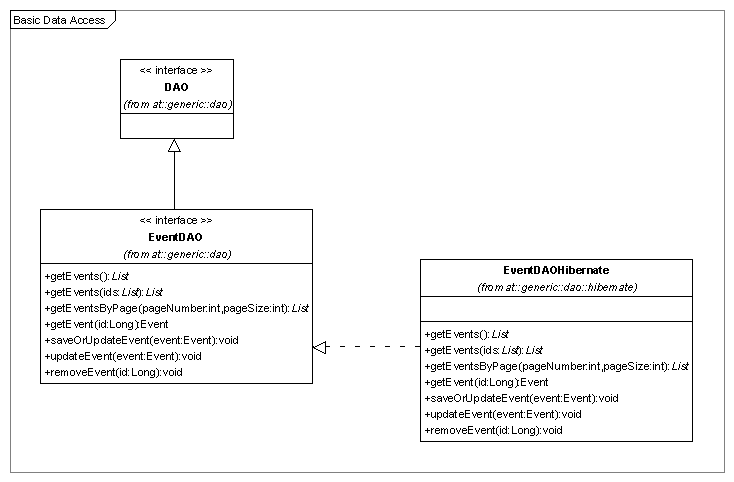
\includegraphics[width=1.0\textwidth]{pics/BasicDataAccess.png}
	\caption{Basic data access for events}             
	\label{fig:BasicDataAccess}
\end{figure}            
%*********************** 
For each of these models there is a DAO interface defined with basic CRUD (create, read, update, delete) methods. Some of them require special methods for different purposes. As the DAO interface is straight forward there is no need to get into details here. The Spring Framework and Hibernate is doing all the hard work. The developer can concentrate on problems situated in the business domain.
\\\\
As Javadoc in combination with UML diagrams is self explanatory, I want to introduce only the basic concepts like the DAO for the event model (Figure \ref{fig:BasicDataAccess}). The DAO forms the central interface from where every other DAO interface is extended. The implementation of the EventDAO is Hibernate specific and is instantiated through Spring's context configuration (Listing Figure \ref{lst:ImplementingDAOInterface})

%***************************************
\begin{figure}[h]  
	\begin{mytinylisting}
	\begin{verbatim}
		<bean id="eventDAOTarget" class="at.generic.dao.hibernate.EventDAOHibernate"> 
		    	<property name="sessionFactory"> 
		    		<ref bean="sessionFactoryForPostgresSource"/> 
		    	</property> 
		</bean>
	\end{verbatim}
	\end{mytinylisting}
	\caption{Implementing DAO interface}             
	\label{lst:ImplementingDAOInterface}
\end{figure} 
%***************************************


%**************************************************************************************
\subsubsection{Persistence Service}
%**************************************************************************************

Event Cloud provides a high level API data access which encapsulates certain operations related to persistence. For example the EventPersistenceService extracts txtime and rwtime, eventtype data and transforms them into the appropriate models and stores them into the according relations using their DAOs. This helps other developers to use the service out of the box without to get into details about persisting events. 
\\\\
The EventPersistenceService is integrated by the Spring Framework using its contex configuration with dependency injection (Listing Figure \ref{lst:EventPersistenceService}). Like almost everywhere the EventPersistenceService also defined as an Interface whose implementation is wired in by the Spring Framework. 
%***********************
\begin{figure}[h!]                                  
	\centering                                           
	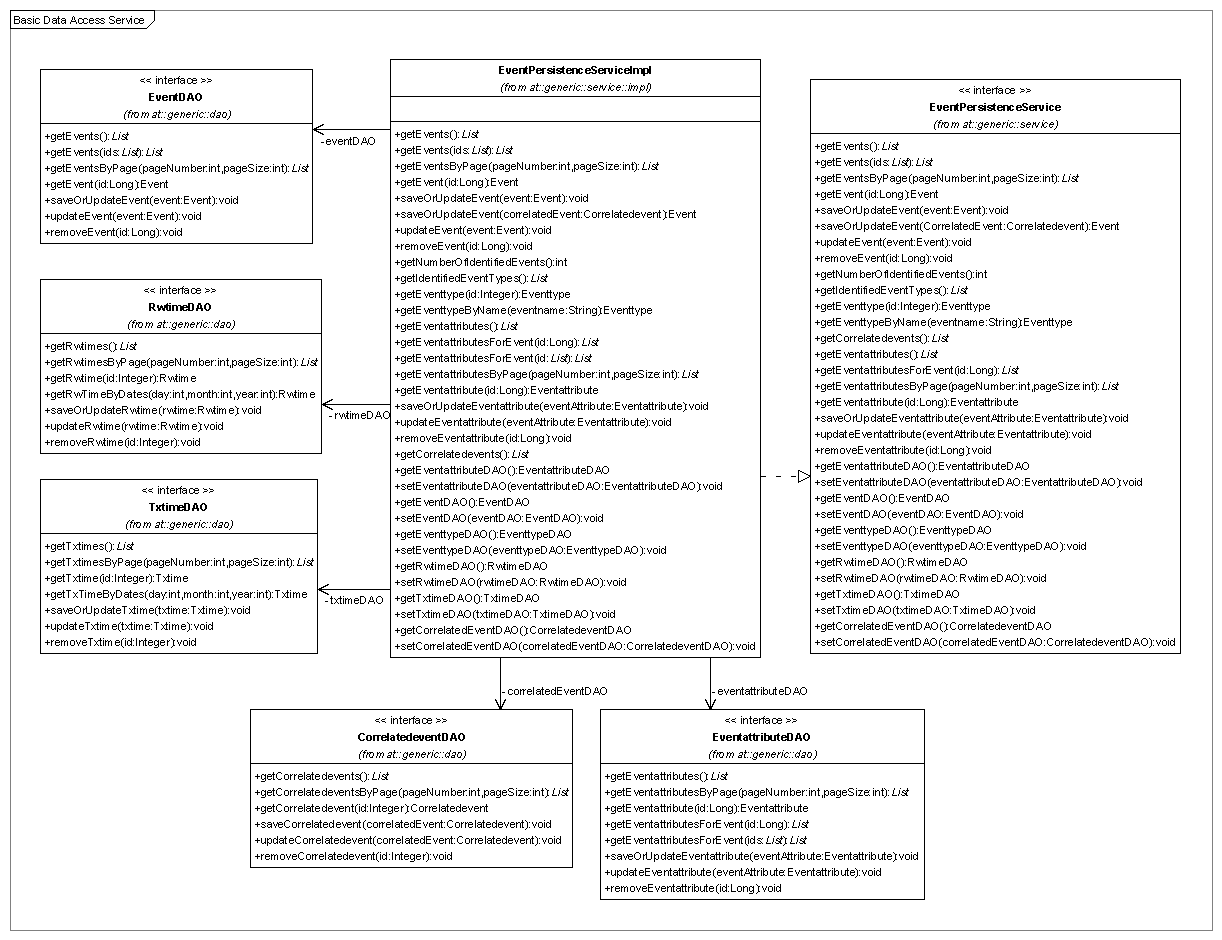
\includegraphics[width=1.0\textwidth]{pics/BasicDataAccessService.png}
	\caption{EventPersistenceService}             
	\label{fig:}
\end{figure}            
%*********************** 

%***************************************
\begin{figure}[h!]  
	\begin{mytinylisting}
	\begin{verbatim}
	<bean id="eventPersistenceService" class="at.generic.service.impl.EventPersistenceServiceImpl"> 
    	<property name="eventDAO">
    		<ref bean="eventDAOTarget"/>
    	</property> 
    	<property name="eventattributeDAO">
    		<ref bean="eventattributeDAOTarget"/>
    	</property> 
    	<property name="eventtypeDAO">
    		<ref bean="eventtypeDAOTarget"/>
    	</property> 
    	<property name="rwtimeDAO">
    		<ref bean="rwtimeDAOTarget"/>
    	</property> 
    	<property name="txtimeDAO">
    		<ref bean="txtimeDAOTarget"/>
    	</property> 
    	<property name="correlatedEventDAO">
    		<ref bean="correlatedEventDAOTarget"/>
    	</property> 
    </bean>
    \end{verbatim}
    \end{mytinylisting}
	\caption{EventPersistenceService Definition}             
	\label{lst:EventPersistenceService}
\end{figure} 

The main persistence service class for the event source database is provided by CorrelatedEventsPersistenceService which is wired into the application the same way as the EventPersistenceService (Figure \ref{fig:CorrelatedEventsPersistenceService} and Listing Figure \ref{lst:EventPersistenceService}).
\\\\
%***********************
\begin{figure}[h!]                                  
	\centering                                           
	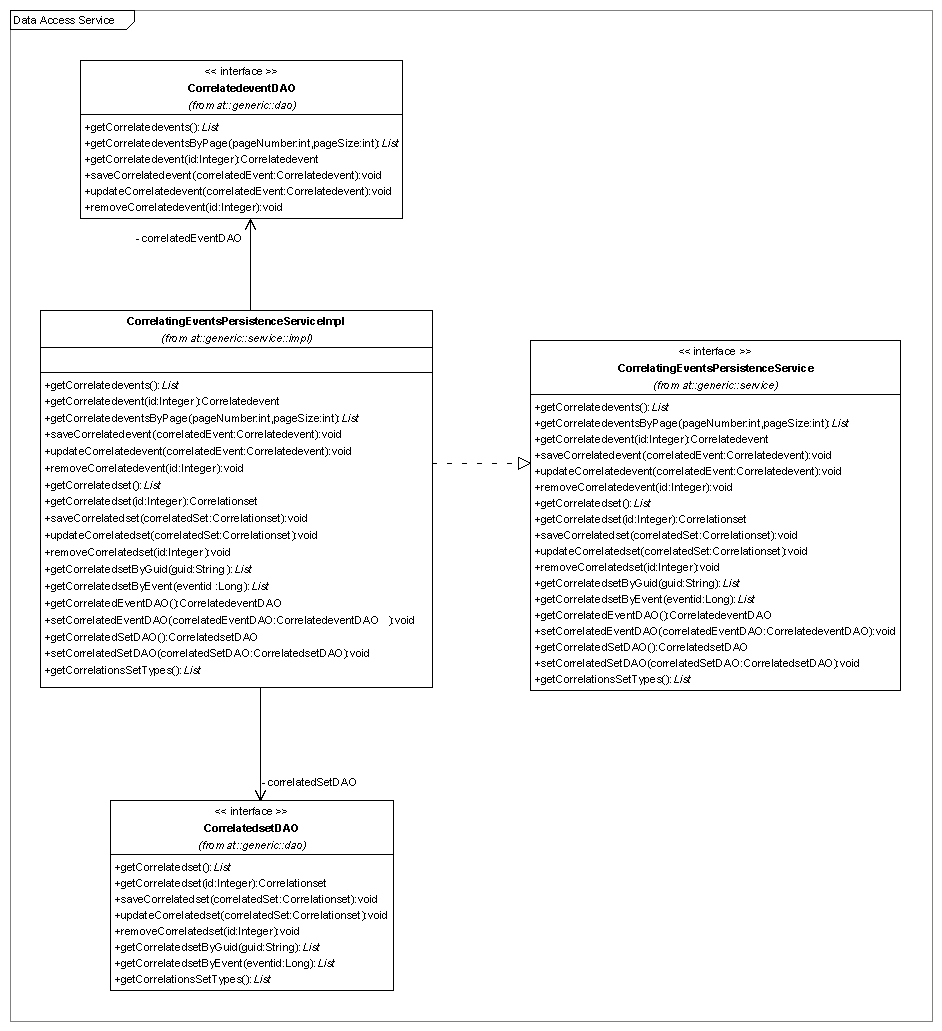
\includegraphics[width=1.0\textwidth]{pics/DataAccessServiceCorrelatedevent.png}
	\caption{CorrelatedEventsPersistenceService}             
	\label{fig:CorrelatedEventsPersistenceService}
\end{figure}            
%***************************************

%***************************************
\begin{figure}[h!]  
	\begin{mytinylisting}
	\begin{verbatim}
	<bean id="correlatingEventsPersistenceService" class="at.generic.service.impl.CorrelatingEventsPersistenceServiceImpl"> 
    	<property name="correlatedEventDAO">
    		<ref bean="correlatedEventDAOTarget"/>
    	</property> 
    	<property name="correlatedSetDAO">
    		<ref bean="correlatedSetDAOTarget"/>
    	</property> 
    </bean>
    \end{verbatim}
    \end{mytinylisting}
	\caption{CorrelatedEventsPersistenceService Definition}             
	\label{lst:EventPersistenceService}
\end{figure} 
%***************************************

The AdminService provides a service for misc. admin operations that has to be persisted including role and filter management for example (Figure \ref{fig:AdminPersistenceService} and Listing Figure \ref{lst:EventPersistenceService}).
\\\\
%***********************
\begin{figure}[h!]                                  
	\centering                                           
	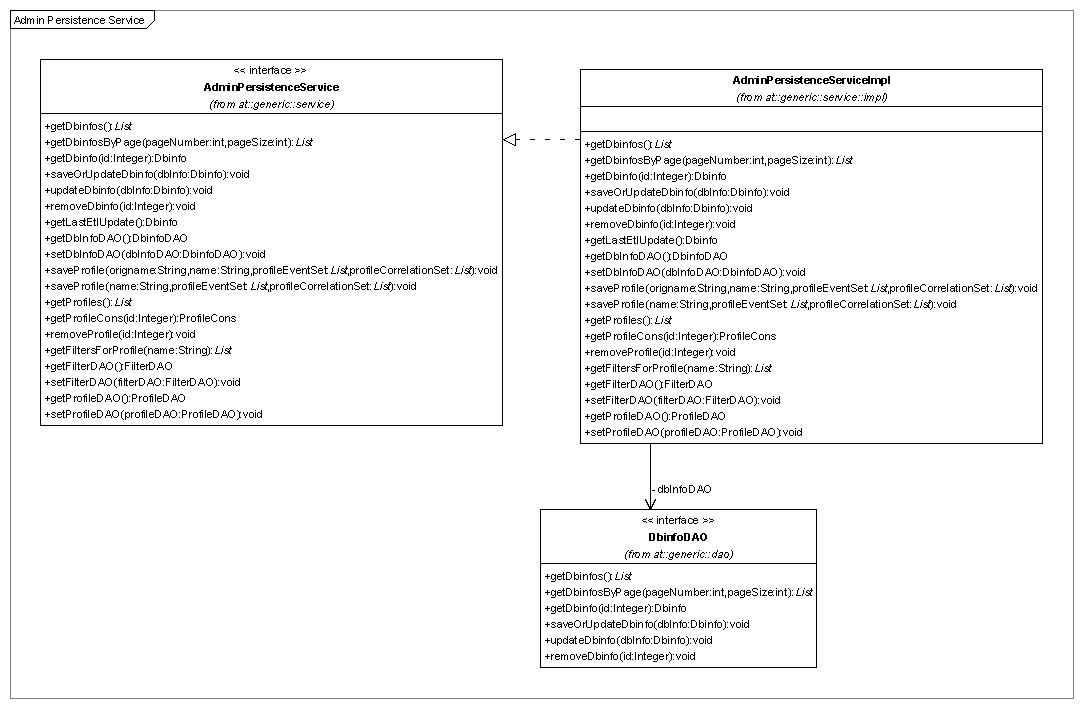
\includegraphics[width=1.0\textwidth]{pics/AdminPersistenceService.png}
	\caption{AdminPersistenceService}             
	\label{fig:AdminPersistenceService}
\end{figure}            
%***************************************

%***************************************
\begin{figure}[h!]  
	\begin{mytinylisting}
	\begin{verbatim}
	<bean id="adminPersistenceService" class="at.generic.service.impl.AdminPersistenceServiceImpl"> 
    	<property name="dbInfoDAO">
    		<ref bean="dbInfoDAOTarget"/>
    	</property> 
    </bean>
    \end{verbatim}
    \end{mytinylisting}
	\caption{EventPersistenceService}             
	\label{lst:EventPersistenceService}
\end{figure} 
%***************************************

%**************************************************************************************
\newpage
\subsection{Loading Process}
%**************************************************************************************
%***********************
\begin{figure}[!h]                                  
	\centering                                           
	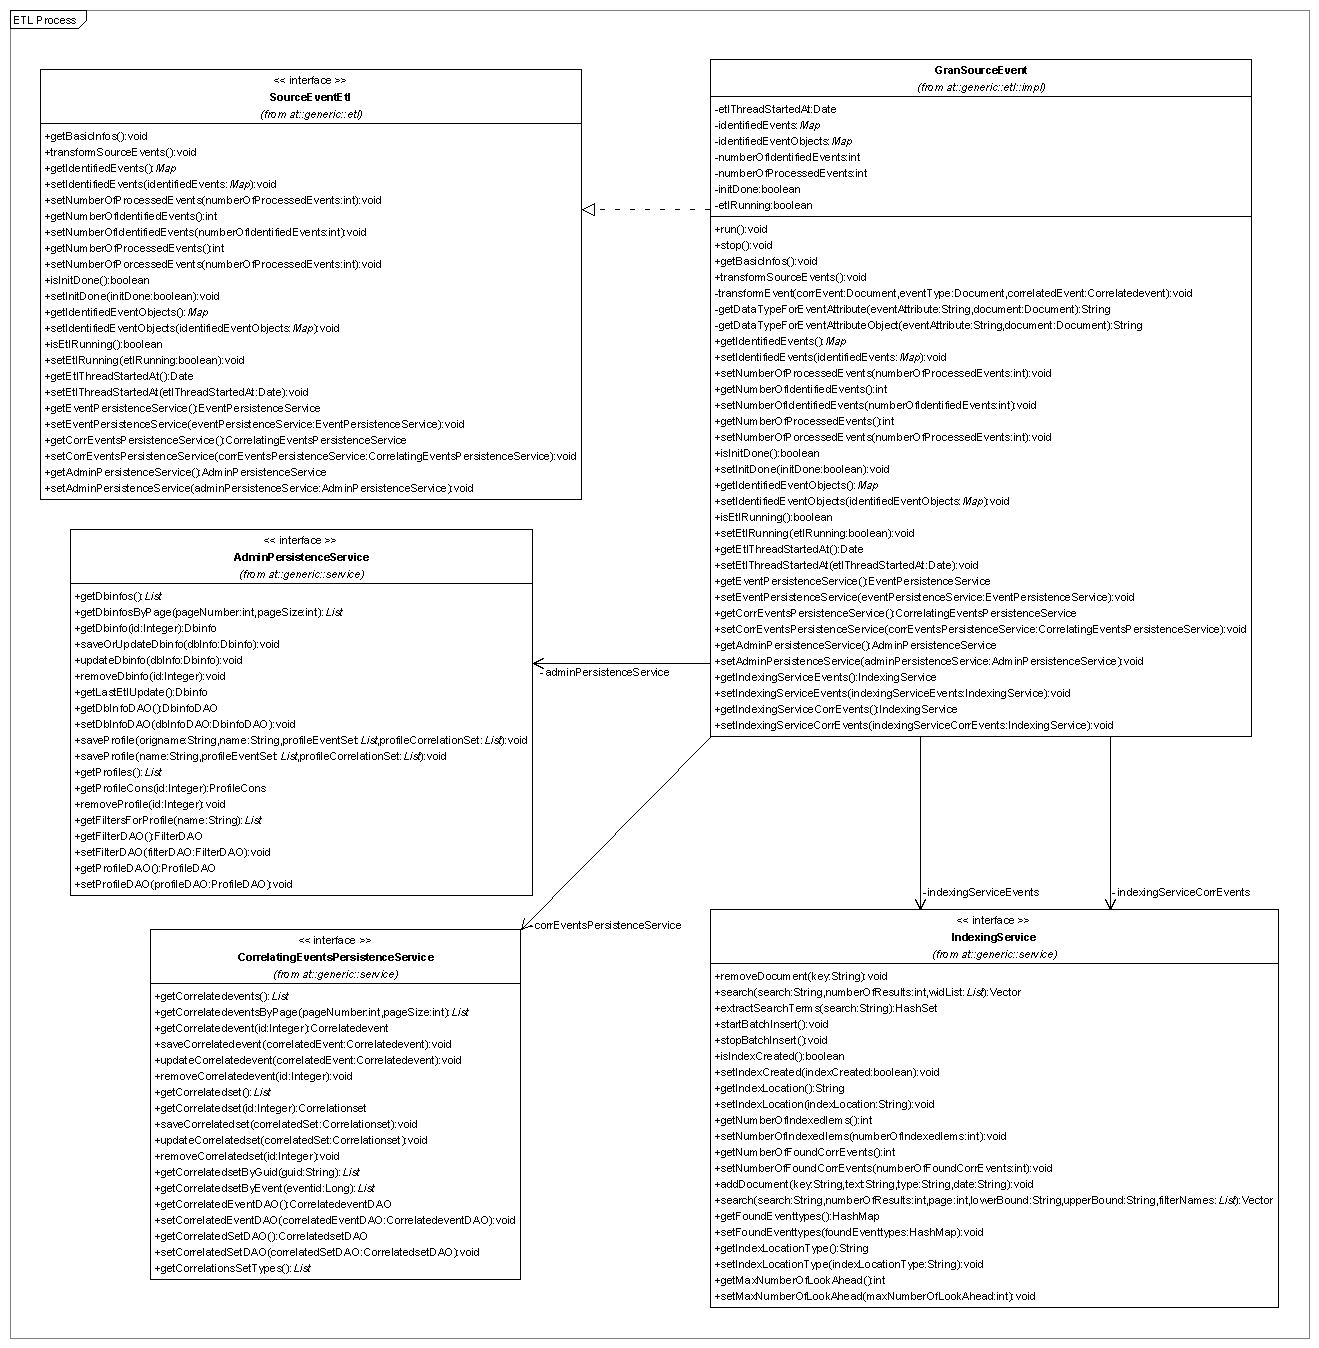
\includegraphics[width=1.0\textwidth]{pics/ETLProcess.png}
	\caption{Loading process}             
	\label{fig:LoadingProcess}
\end{figure}            
%***************************************
The Intime database provides the events with different information (Listing Figure \ref{lst:SourceEvent}). Each event comes with a unique id, a creation time and the event itself as an xml. The attributes from the OrderReceived root node are basic key-value pairs that are stored straight forward into the events relation. 
\\\\
The more tricky part is the extraction of each attribute and their validation against its definition. The datatypes of each attribute are extracted and stored into the database as well. A lot of work in this process is done by the EventPeristenceServices as it automatically takes care about saving eventtypes and timepoints. 
\\\\
This process is pretty straight forward as the user only has to provide event definitions and register the new events in Spring's context configuration. The user can control and supervise the loading process from the web user interface in the admin section. By clicking the button ``Start Transformation'' a thread is triggered that is collecting the events from it source and transforms them into the target database schema. During this process the full text index is created or update which is done by using the Indexer interface (Figure \ref{fig:etlProcess}).

% TODO: screenshot vom adminteil reingeben 

%***************************************
\begin{figure}[h!]  
	\begin{mytinylisting}
	\begin{verbatim}
	<OrderReceived 
		guid="ec3db221-3f65-48cc-9982-7bf781fab3b7" 
		originalGuid="8f2cf907-5e5f-4f0c-8aa8-e07ab521d1a9" 
		priority="Medium" severity="Unknown" 
		localTimeCreated="2006-03-04T17:31:29.6085000+01:00" 
		localTimeCreatedRW="2006-03-04T17:31:29.6085000+01:00" 
		utcTimeCreated="2006-03-04T16:31:29.6085000+01:00" 
		utcTimeCreatedRW="2006-03-04T16:31:29.6085000+01:00" 
		majorVersion="1" 
		minorVersion="0">
		
		<OrderId>1000</OrderId>
		<DateTime>2005-11-01T07:00:00.0000000+01:00</DateTime>
		<DeliveryDate>2005-11-07T15:47:00.0000000+01:00</DeliveryDate>
		<Destination>Paris</Destination>
		
		<ProductCollection>
			<Product>
				<ProductId>Arzeutic</ProductId>
				<Amount>800</Amount>
			</Product>
		</ProductCollection>
	</OrderReceived>
    \end{verbatim}
    \end{mytinylisting}
	\caption{Source Event}             
	\label{lst:SourceEvent}
\end{figure} 
%***************************************

%***********************
\begin{figure}[!h]                                  
	\centering                                           
	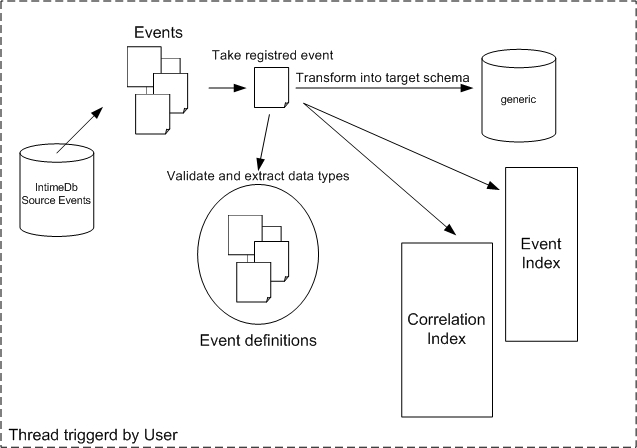
\includegraphics[width=1.0\textwidth]{pics/etlProcess.jpg}
	\caption{ETL Process}             
	\label{fig:etlProcess}
\end{figure}            
%***************************************

%**************************************************************************************
\subsection{Spring IoC Container}
%**************************************************************************************
During the time when Java programming reached its critical mass of users Sun Microsystems published the Enterprise Java Beans 1.0 specifications in 1998. EJB is a server side component settled in the middle layer of an enterprise application. Its major goal is to improve distribution transparency and reusability of components underlined by the statement that EJBs should make developing enterprise systems easier. EJB actually was the first technology that allowed decelrative transactions for instance. 
\\\\
As time went by the first enthusiasm had gone and experiences with EJB have shown that they don't necessarily hold what they promised. This problem has been addressed by Rod Johnson in first place (\cite{Johnson02}). EJB addresses just too many problems thus results in a high complexity. As most applications don't need the most addressed features EJBs create too much overhead. 
\\\\
Rod Johnson propagates following major flaws of EJBs based on his experience \cite{Johnson02}:
\begin{itemize}
	\item It brings too much unnecessary complexity with it.
	\item Through EJB's complexity provided the productivity is low and the probability of erros grow.
	\item Automated unit testing is poorly supported.
	\item Huge amounts of problem specifications have been worked out, but only a slight percentage addresses common real world problems.
	\item Entity Beans have failed.
	\item EJB system have a relatively poor performance and don't scale up well.
	\item Too much code has to be produced which resulted in various code generators that make maintainability problematic.
	\item EJBs promised to be platform independent. In reality applications became EJB container vendor specific.
\end{itemize}

The quesion arises ``Why use J2EE and EJBs at all then?''. The answer is that J2EE provides a wide range of useful services and standards that can be integrated into applications without the use of EJBs. Spring's goal is to deliver those services to the user by simplifying the programming model using only simple POJOS (\cite{SpringInAction05}).
\\\\
\textit{Spring is a lightweight inversion of control and aspect-oriented container framework.} \cite{SpringInAction05}
\\\\
Spring is acutally a lightweight container that provides an inversion of control (IoC). This means that it is capable of managing the life cycle and configuration of its beans. The inversion of control pattern makes it possible to write the applications business logic completle unaware of its underlying technology. Spring provides means of creating dependencies without any intrusion into business code. That is a major feature which allows to develop loosely coupled and highly scalable components. The developer can concentrate on solving business problems and creating easily reusable components. It is possible to remove the complete Spring support from the application without affecting any business code written. Using the Spring Framework the developers are forced to program against interfaces and the concrete implementation of the code is wired in, by configuration files, using Spring. Another enriching feature is that Spring makes extensive use of the aspect oriented programing (AOP) paradigm which is used to separate business logic from system services like transaction management seen the previous section. The transaction management of the data access is completely separated from the code and even the Hibernate specific implementation parts can be changed in a minute using the configuration power of Spring. 
\\\\
The Spring Framework is composed of several main components:
\begin{itemize}
	\item Core container
	\item O/R Mapping modules
	\item Application Context Modules
	\item JDBC and DAO modules
	\item MVC Framework
\end{itemize}

The core of the Spring Framwork is undisputable the core container and the application context module. The core containers heart is the BeanFactory which lets the user wire the components together. It uses the Factory Pattern to realize dependency injections and to control the objects life cycles. The BeanFactory supports two types of objects: Singelton and Prototype. The Singelton creates a shared instance of an object which is addressed by a name and mostly used as an stateless object. The Prototype allows to create an independent instance for each reference of this class.
\\\\
The O/R and DAO modules have been discussed in detail in the previous sections.
\\\\
The business logic should always be laid inside simple Java Beans with according getters and setters to its dependent objects to enable the dependency injection by the BeanFactory. These beans are implemented against a previously defined interface. For example the SearchService is an interface to a Java Bean that has got references to other beans with according getters and setters. These beans are defined in the application context and their implementations and dependencies are wired together using the Spring Framework (Listing Figure \ref{lst:wiringbeanstogether}).

%***************************************
\begin{figure}[h!]  
	\begin{mytinylisting}
	\begin{verbatim}
	<bean id="indexingServiceCorrEvents" class="at.generic.search.impl.LuceneIndexingImpl" init-method="init"> 
	    	<property name="indexLocation">
	    		<value>d:/luceneindex/correvents</value>
	    	</property> 
	</bean>    

 	<bean id="searchService" class="at.generic.search.impl.SearchServiceImpl"> 
    	<property name="indexingServiceCorrEvents">
    		<ref bean="indexingServiceCorrEvents"/>
    	</property> 
    	<property name="indexingServiceEvents">
    		<ref bean="indexingServiceEvents"/>
    	</property> 
    	 <property name="eventPersistenceService">
    		<ref bean="eventPersistenceService"/>
    	</property> 
    	<property name="corrPersistenceService">
    		<ref bean="correlatingEventsPersistenceService"/>
    	</property>
    	<property name="maxSearchResults">
    		<value>10</value>
    	</property>
    </bean>    
    \end{verbatim}
    \end{mytinylisting}
	\caption{Wiring beans together.}             
	\label{lst:wiringbeanstogether}
\end{figure} 
%***************************************
% *********************
% TODO:
% - IoC und AOP genauer beschreiben!
% ******************
%**************************************************************************************
\subsection{Spring MVC}
%**************************************************************************************
The MVC pattern was originally introduced in Smalltalk developed in the 70s at the Xerox Palo Alto Research Center. Its main purpose was to manage the GUI and user interactions for the first graphic-window based applications. The MVC pattern is used to seperate the representation, processing and data components to achieve a loosely couple design which results in a clean reusable and maintainable code. 
\\\\
The three main seperations are:
\begin{itemize}
	\item \textbf{Model:} Represents the underlying domain models which are usually populated by a database like in Event Cloud the event models.
	\item \textbf{View:} This component is mainly responsible for presenting the data and the user interface. In a webbase application this is normally done using JSP/JSTL to render HTML pages containing some data.
	\item \textbf{Controller:} This is the core component which handles the coordination. It is responsible of processing user inputs, delegating requests to business processes and coordinating the representation of results.
\end{itemize}
Spring Framework brings a full blown MVC framework with it to help to develop web applications in a fast and efficient way. Spring's MVC comes with a rich set of features:

\begin{itemize}
	\item automatic population of models according to request parameters
	\item declarative validation
	\item state management through web forms
	\item workflow coordination
\end{itemize}

Spring's MVC life cycle is presented in the Figure \ref{fig:SpringMVC}. The DispatcherServlet is receiving user requests and queries the according mapping for the specific request. The HandlerMapping is simply mapping URLs to controllers. The Dispatcher is delegating the request to the according controller once it resolved the mapping. The Controllers job is to perform some business operations in sense that it delegates the workload to business objects like the service API provided by Event Cloud. After work has been done the Controller populates so called ``Command Models'' that hold all information, that is needed to be shown to the user, and returns a ModelAndView object to the Dispatcher that contains the command model and a view name. The ViewResolver is then responsible to resolve the viewname and map it to the according view. In Event Clouds case this is a JSP page which only performs JSTL operations with display formatting routines to generate the desired HTML rendered information to its user. 
\\\\
An important feature that Spring MVC provides is that it is possible to create interceptors for specific mappings and controllers comparable to servlet filters. This allows to implement access control for instance in no time and without to touch any controller. This provides an extremely loosely coupled design as no code is touched when implementing such a thing.   
\\\\
%***********************
\begin{figure}[!h]                                  
	\centering                                           
	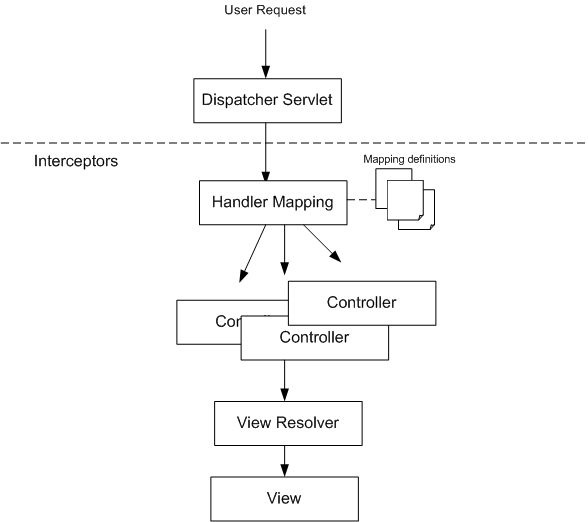
\includegraphics[width=1.0\textwidth]{pics/SpringMVC.jpg}
	\caption{Spring MVC}             
	\label{fig:SpringMVC}
\end{figure}            
%***************************************

To give a clear picture how this works in Event Cloud there is a Listing Figure \ref{lst:urlMapping} provided for understanding the principle of configuring Spring's MVC in Event Cloud. The first one shows how the controllers are mapped to a requested URLs. For matter of simplicity only the process of resolving the Event Clouds admin page is explained.  The admin's controller is bind to a specific object which takes several bean dependencies as arguments. The admin controller itself does not perform any business logic. It just determines what kind of request got in and decides which operation should be executed like the etl process or the creation of filter profile. Afterwards it creates an instance of a command object that holds the data to be displayed for example which Events have been identified, when the last update process has been executed and stuff like that. When finished performing business operations it returns a ModelAndView object including the according view name to be resolved and the name of the command object that is used by the jsp page to access it (Listing Figure \ref{lst:MVCByAdminController}). 
\\\\
The openSessionInViewInterceptor used in this excerpt is a workaround to provide access for lacy loading in the view component.

\begin{figure}[h!]  
\begin{mytinylisting}
\begin{verbatim}
	<!bean id="urlMapping"     
			class="org.springframework.web.servlet.handler.SimpleUrlHandlerMapping"> 
		<property name="interceptors">
	        <list>
				<!-- Interceptor f�r Lacy Loading im View -->
	             <ref bean="openSessionInViewInterceptor"/>
	        </list>
		</property>
       	<property name="mappings">
			<props>
				<prop key="/admin.html">adminController</prop>
			</props>
		</property>
	</bean>
	
	<bean name="adminController" class="at.generic.web.AdminController">
  		<property name="sourceEventEtl">
			<ref bean="sourceEventEtl"/>
		</property>
		<property name="adminPersistenceService">
			<ref bean="adminPersistenceService"/>
		</property>
		<property name="eventPersistenceService">
			<ref bean="eventPersistenceService"/>
		</property>
		<property name="indexingServiceEvents">
			<ref bean="indexingServiceEvents"/>
		</property>
		<property name="indexingServiceCorrEvents">
			<ref bean="indexingServiceCorrEvents"/>
		</property>
  	</bean>
    \end{verbatim}
    \end{mytinylisting}
	\caption{URL Mapping}             
	\label{lst:urlMapping}
\end{figure} 
%********************

%********************
\begin{figure}[!h]  
\begin{mytinylisting}
\begin{verbatim}
	return new ModelAndView("admin", "adminData", adminData);
    \end{verbatim}
    \end{mytinylisting}
	\caption{ModelAndView returned by the AdminController}             
	\label{lst:MVCByAdminController}
\end{figure} 
%********************

%**************************************************************************************
\subsection{Indexing and Searching Events}
%**************************************************************************************
%**************************************************************************************
\subsubsection{Indexing Events with Lucene }
%**************************************************************************************
Lucene\footnote{http://lucene.apache.org/} is an open source high performance full text indexing and search library completle written in Java. Originally developed by Cutting 2001 it became a popular piece of software which is now maintained and extended by volunteers as a Jakarta project. During the development of Event Cloud, Lucene release its 1.9 version which was a major step in its development. The group is looking forward to introduce the 2.0 version of its software. Lucene provides a high performance indexing implementation and offers a sophistacted search algorithm. The main power of Lucene is actually its search implementation including its Ranking algorithm that yields excellent search results. Lucene is suitable for almost every application that needs some kind of text indexing. Originally it was used to index data and information provided for example on webpages or documents. It provides several libraries to parse different formats like pdf, doc or XMLs. However people started to use Lucene to index their databases as well to provide an efficient and fast full text search for their applications. Lucene provides the possibility to store metadata with the given documents that can be indexed by choice such as author, title or date of creation. This provides a powerfull alternative of managing and saving data for search centric applications. Lucene can create an index either on disk or it can build an extremely fast transient index in memory. 
\\\\
The real benefit developers can take from Lucene is its extremely well designed architecture. The developer has to be familiar with only a handful of classes in order to implement a rudimentary index and search application. 
\\\\
There are basically two core classes of Lucene that the developer has to know in detail:
\begin{itemize}
	\item \textbf{IndexWriter} for creating and upating an index
	\item \textbf{IndexSearcher} for searching an index
\end{itemize}

How simple it can be to create a basic index and add a document to it is shown in the Listing Figure \ref{lst:SimpleIndexWithLucene}. A simple search example is presented in the Listing Figure \ref{lst:SimpleSearchWithLucene}
%********************
\begin{figure}[!h]  
	\begin{mytinylisting}
	\begin{verbatim}
	IndexWriter writer = new IndexWriter(indexLocation, analyzer, false);
	writer = new IndexWriter(indexLocation, analyzer, false);
			
	Document document = new Document();
	document.add(Field.Keyword("author", author));
	document.add(Field.Keyword("title", title));
	document.add(Field.Text("content",content));
		    
	writer.addDocument(document);
	writer.optimize();
	writer.close();
    \end{verbatim}
    \end{mytinylisting}
	\caption{Example of creating a simple index with Lucene.}             
	\label{lst:SimpleIndexWithLucene}
\end{figure} 
%********************

%********************
\begin{figure}[!h]  
	\begin{mytinylisting}
	\begin{verbatim}
	
	Directory fsDir = FSDirectory.getDirectory(indexLocation, false);
    IndexSearcher indexSearcher = new IndexSearcher(fsDir);
    
    Query query = QueryParser.parse(searchString.trim(), "content", new StandardAnalyzer());
    Hits hits = indexSearcher.search(query);
	
	\end{verbatim}
    \end{mytinylisting}
	\caption{Example of searching through an index with Lucene.}             
	\label{lst:SimpleSearchWithLucene}
\end{figure} 
%********************

However indexing and searching for events and their correlations in Event Cloud requires a bit more complex algorithms. The next sections will provide the main concepts implemented for searching and retrieving those events. Event Cloud provides another API service, like the persistence service classes, for indexing and retrieving event information to simplify the use of Event Clouds underlying mechanisms and to provide another layer of abstraction. 
\\\\
A central role in the indexing process has the IndexingService interface that provides the common methods to EventCloud and the LuceneIndexingImpl for the concrete Lucene implementation (Figure \ref{fig:IndexingService}). These classes are wired together using Spring's application context like everywhere else in Event Cloud. 
\\\\
%***********************
\begin{figure}[!h]                                  
	\centering                                           
	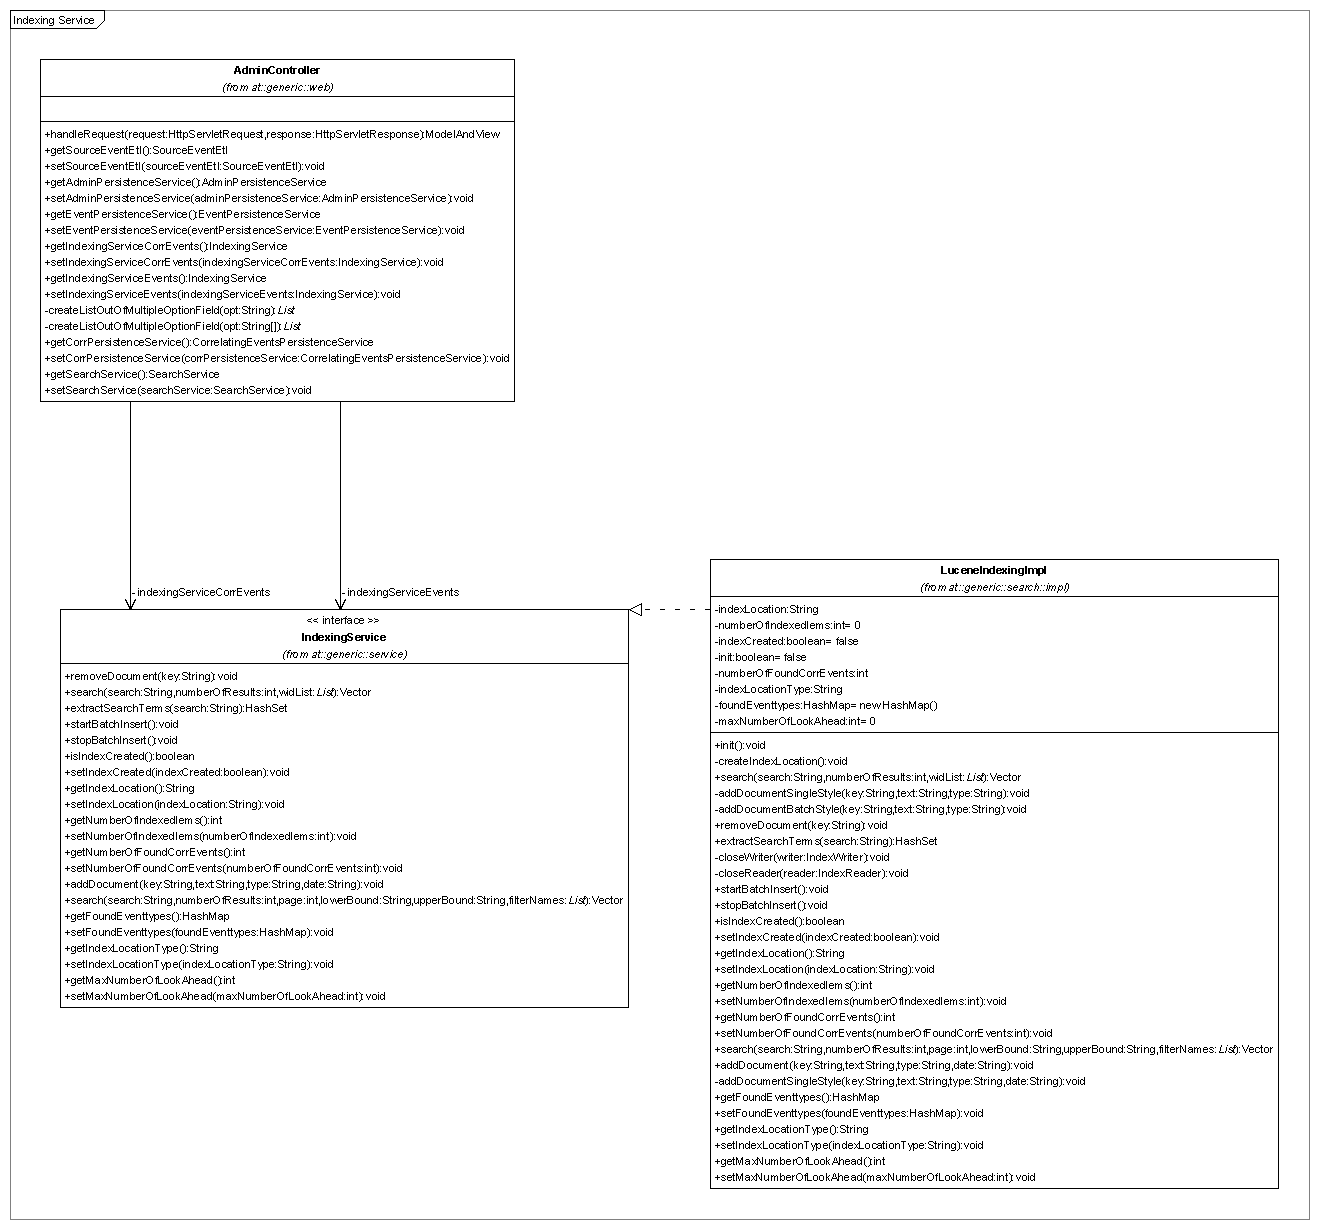
\includegraphics[width=1.0\textwidth]{pics/IndexingService.png}
	\caption{IndexingService}             
	\label{fig:IndexingService}
\end{figure}            
%***************************************

In the provided Figure \ref{fig:IndexingService} the AdminController is inserted to show that there are two instances of  the IndexingService created. This is because there is one index only for events and one index for retrieving correlations. The decision has been made to boost up search performance as one index powers the Rank 1 search type and the other index powers the Rank 2 search. Putting both information into one index would result in an unnecessary overhead. 
\\\\
The index locations are provided by as parameters in the Event Clouds context configuration. 
\\\\
The index creation itself is performed during the loading and transformation process triggered by the user. While the ETL process is transforming and storing the events to the database it creates the index for the events. When the event processing is finished a correlation index is built out of the correlation information provided by the Intime database (Figure \ref{fig:LoadingProcess})
\\\\
%***********************
\begin{figure}[!h]                                  
	\centering                                           
	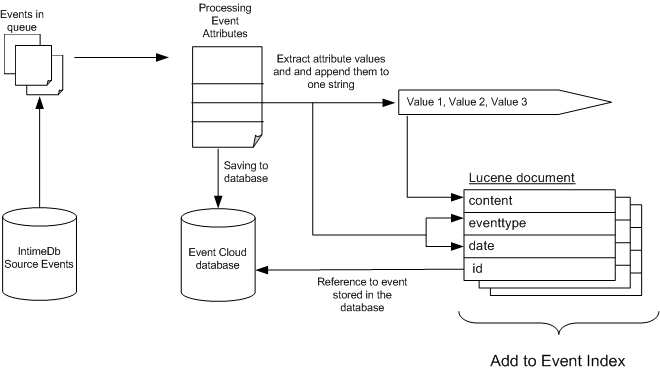
\includegraphics[width=1.0\textwidth]{pics/indexingProcessFromEtl.jpg}
	\caption{Indexing an Event.}             
	\label{fig:IndexingAnEvent}
\end{figure}    
%***************************************        
The event Lucene document that is added to the event index, is consisting of four attributes (Figure \ref{fig:IndexingAnEvent}):

\begin{itemize}
	\item \textbf{content:} While the event attributes are processed by the transformation service each value of the attributes are extracted and appended to a string variable. This string contains every value from the event's attributes and is comparable to a document's text. This string is indexed.
	\item \textbf{eventtype:} This contains the eventype that is extracted during the transformation process. This field is not indexed.
	\item \textbf{date:} This field contains the events date and is indexed.
	\item \textbf{id:} This field is not indexed and is stored to the document to preserve the connection to the event and its attributes in the database. This is used for various operations during the search process. If an event has been found through its content and the document is retrieved it is possible to step into the relational world and retrieve other information or make use of the relational databases advantages for other purposes.
\end{itemize}

%***********************
\begin{figure}[!h]                                  
	\centering                                           
	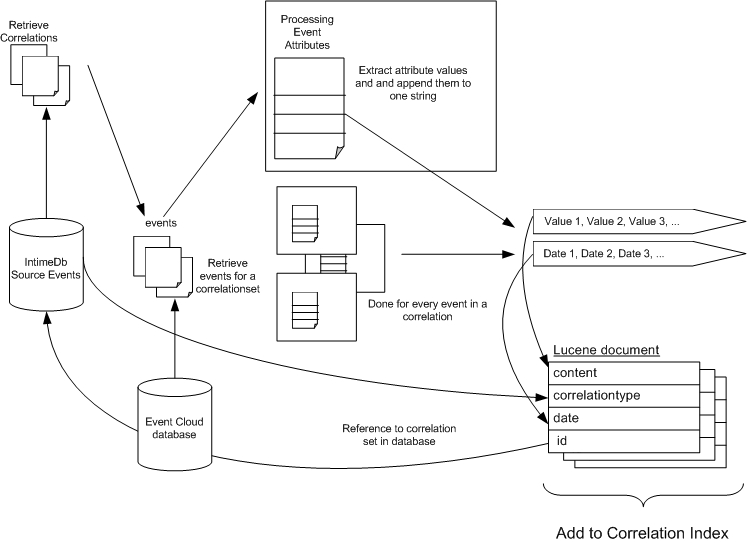
\includegraphics[width=1.0\textwidth]{pics/indexingProcessFromEtlCorrEvents.jpg}
	\caption{Indexing a Correlation.}             
	\label{fig:IndexingACorrelatioin}
\end{figure}    
%***************************************    

The correlation index is slightly different than the event index created. The document types are the same but have different contents (Figure \ref{fig:IndexingACorrelatioin}):

\begin{itemize}
	\item \textbf{content:} The content contains, in contrast to the event's content field, all attribute values from the events that belong to a correlation. These correlations are fetched from the source database and all events belonging to a correlation are retrieved from Event Cloud's database and their attributes are extracted and stored into a string. This time every event attributes value, belonging to the currently processed correlation, is stored into the content string which is then indexed.
	\item \textbf{eventtype:} The eventtype field is unindexed and this time it contains the correlation type. 
	\item \textbf{date:} This field is different too as every events date is appended to the date field that belongs to a correlation. This is done the same way as the content field is create, but this time event date information are stored and not attribute values. This is necessary for the date filter used in the search process. Lucene comes with a filter features that allows to create a date filter on those kind of stored dates as they are stored internally as coded character streams.
	\item \textbf{id:} The id references the original correlation in the source database and is not indexed in here as well.
\end{itemize}

%**************************************************************************************
\subsubsection{Searching for Events}
%**************************************************************************************

Now comes the main application of Event Cloud - the search for events and their applications. As we have seen previously there are two Rank types implemented. The first one, is a simple event search and the second one is the search over correlations. First I want to introduce the search capabilities from the users point of view and then get into implementation details. 
\\\\
The Figure \ref{fig:mainView} shows two options and an input field for the search query. The option ``over correlation sets'' equals the Rank 2 search and the option ``only events'' equals the Rank 1 search. 
\\\\
%***********************
\begin{figure}[!h]                                  
	\centering                                           
	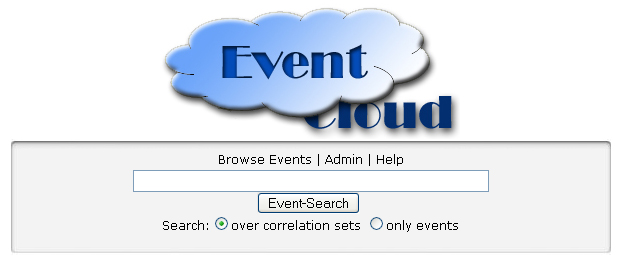
\includegraphics[width=1.0\textwidth]{pics/screenshots/mainView.jpg}
	\caption{Main View}             
	\label{fig:mainView}
\end{figure}    
%*************************************** 

The Figure \ref{fig:Rank2SearchScreenshot} shows how the correlation results are represented. The middle frame shows the correlation search results ordered by their hit relevance. The Hits have been calculated by Lucenes ranking algorithm and underneath there are several events presented that matched the search query. This is an important topic as there are actually two aggregation levels of results presented. The first level is the correlationset that best matched the search query and underneath the most relevant events are displayed that matched the query (Figure \ref{fig:Rank2SearchHits}). The other events belonging to that correlation are hidden as they did not matched the query. By pressing the ``plus'' button next to correlation's name all events can be displayed that belong to that correlationset. By clicking on an event the right handed panel is displayed with details about the event. The event details can be represented either as the raw event xml or in a more human readable way as styled tables. The panel on the left hand side can be faded in by clicking on the ``more options'' button. This is the filter bar where the user can consequently remove correlationtypes from the result set, apply a date range filter or a previously created profile in the admin section. 
\\\\
%***********************
\begin{figure}[!h]                                  
	\centering                                           
	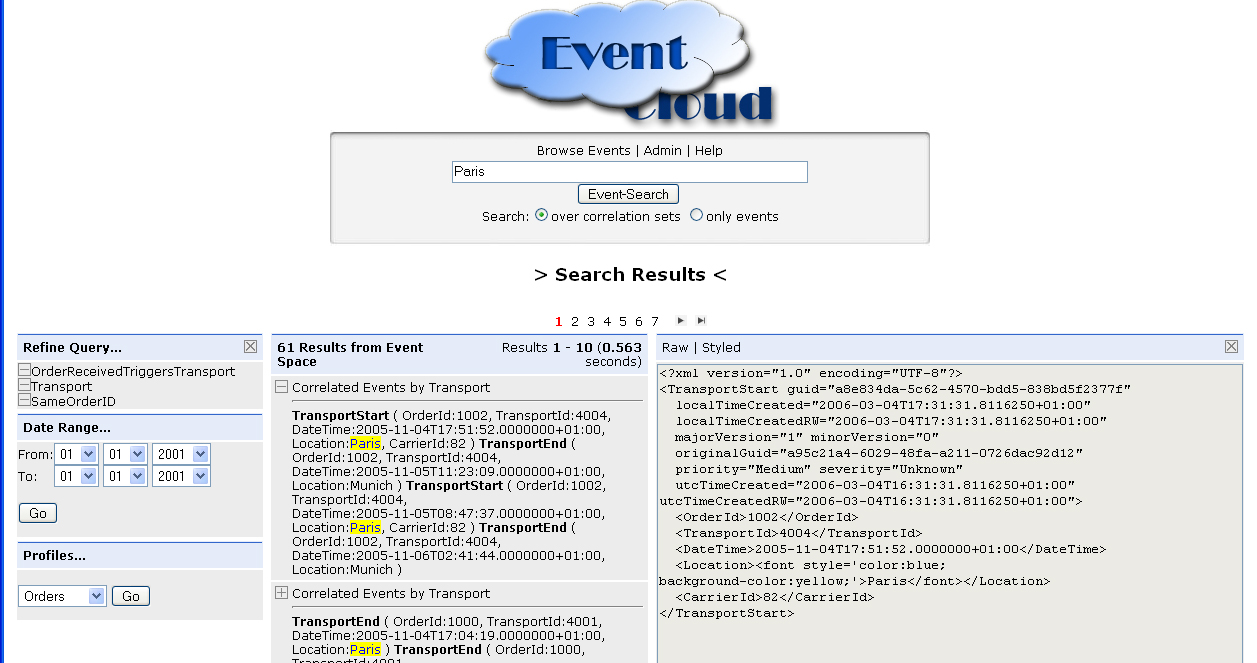
\includegraphics[width=1.0\textwidth]{pics/screenshots/EventDetails.jpg}
	\caption{Rank 2 search screenshot}             
	\label{fig:Rank2SearchScreenshot}
\end{figure}    
%*************************************** 

%***********************
\begin{figure}[!h]                                  
	\centering                                           
	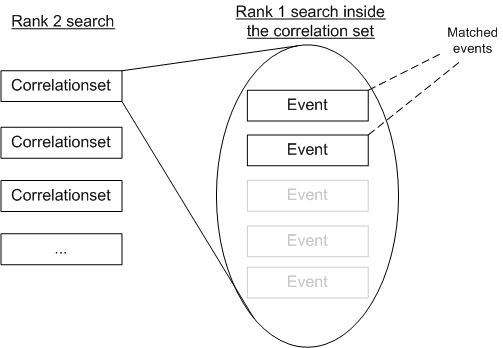
\includegraphics[width=1.0\textwidth]{pics/Rank2SearchHits.jpg}
	\caption{Rank 2 search hits}             
	\label{fig:Rank2SearchHits}
\end{figure}    
%*************************************** 

The Rank 1 search provides the same features with the difference that there is only the Rank 1 search performed and thus only events are presented ranked by Lucene (Figure\ref{fig:Rank1SearchHits}). 
\\\\
%***********************
\begin{figure}[!h]                                  
	\centering                                           
	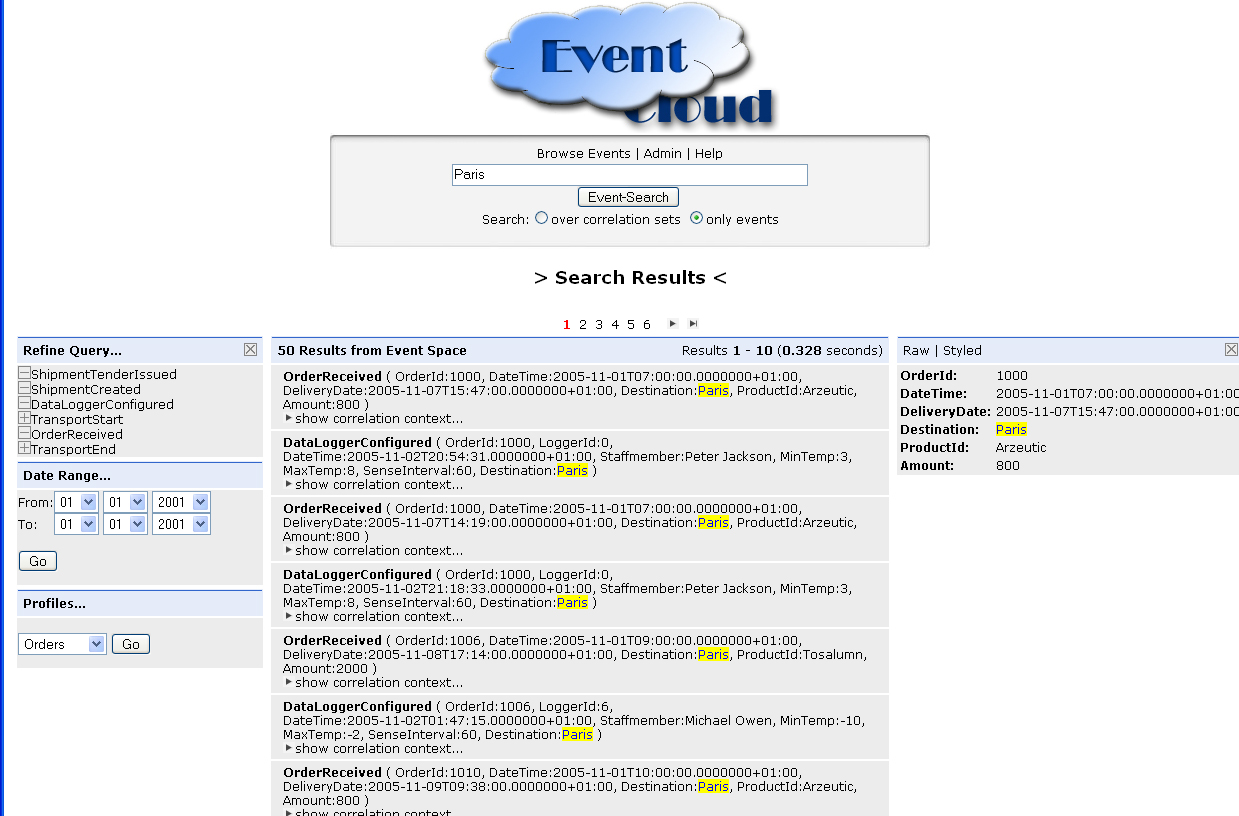
\includegraphics[width=1.0\textwidth]{pics/screenshots/eventDetailsEventSearch.jpg}
	\caption{Rank 1 search hits}             
	\label{fig:Rank1SearchHits}
\end{figure}    
%*************************************** 

The real interesting things happen in the background. Event Cloud provides another Service API which is used for searching the indexes. The search is triggered by the user and processed by the SearchController. The SearchController is the main class for coordinating the search and managing the result interface which is currently quite complex to provide an interactive look and feel like many AJAX applications provide. There was a discussion about implementing the interface using AJAX but this idea has been dismissed as there is no defacto standard AJAX library around. You can find tons of free AJAX libraries that are more or less good. Event Cloud should provide the basic infrastructure for further work so it made no sense to apply volatile frameworks that could become obsolete tomorrow. 
\\\\
%***********************
\begin{figure}[!h]                                  
	\centering                                           
	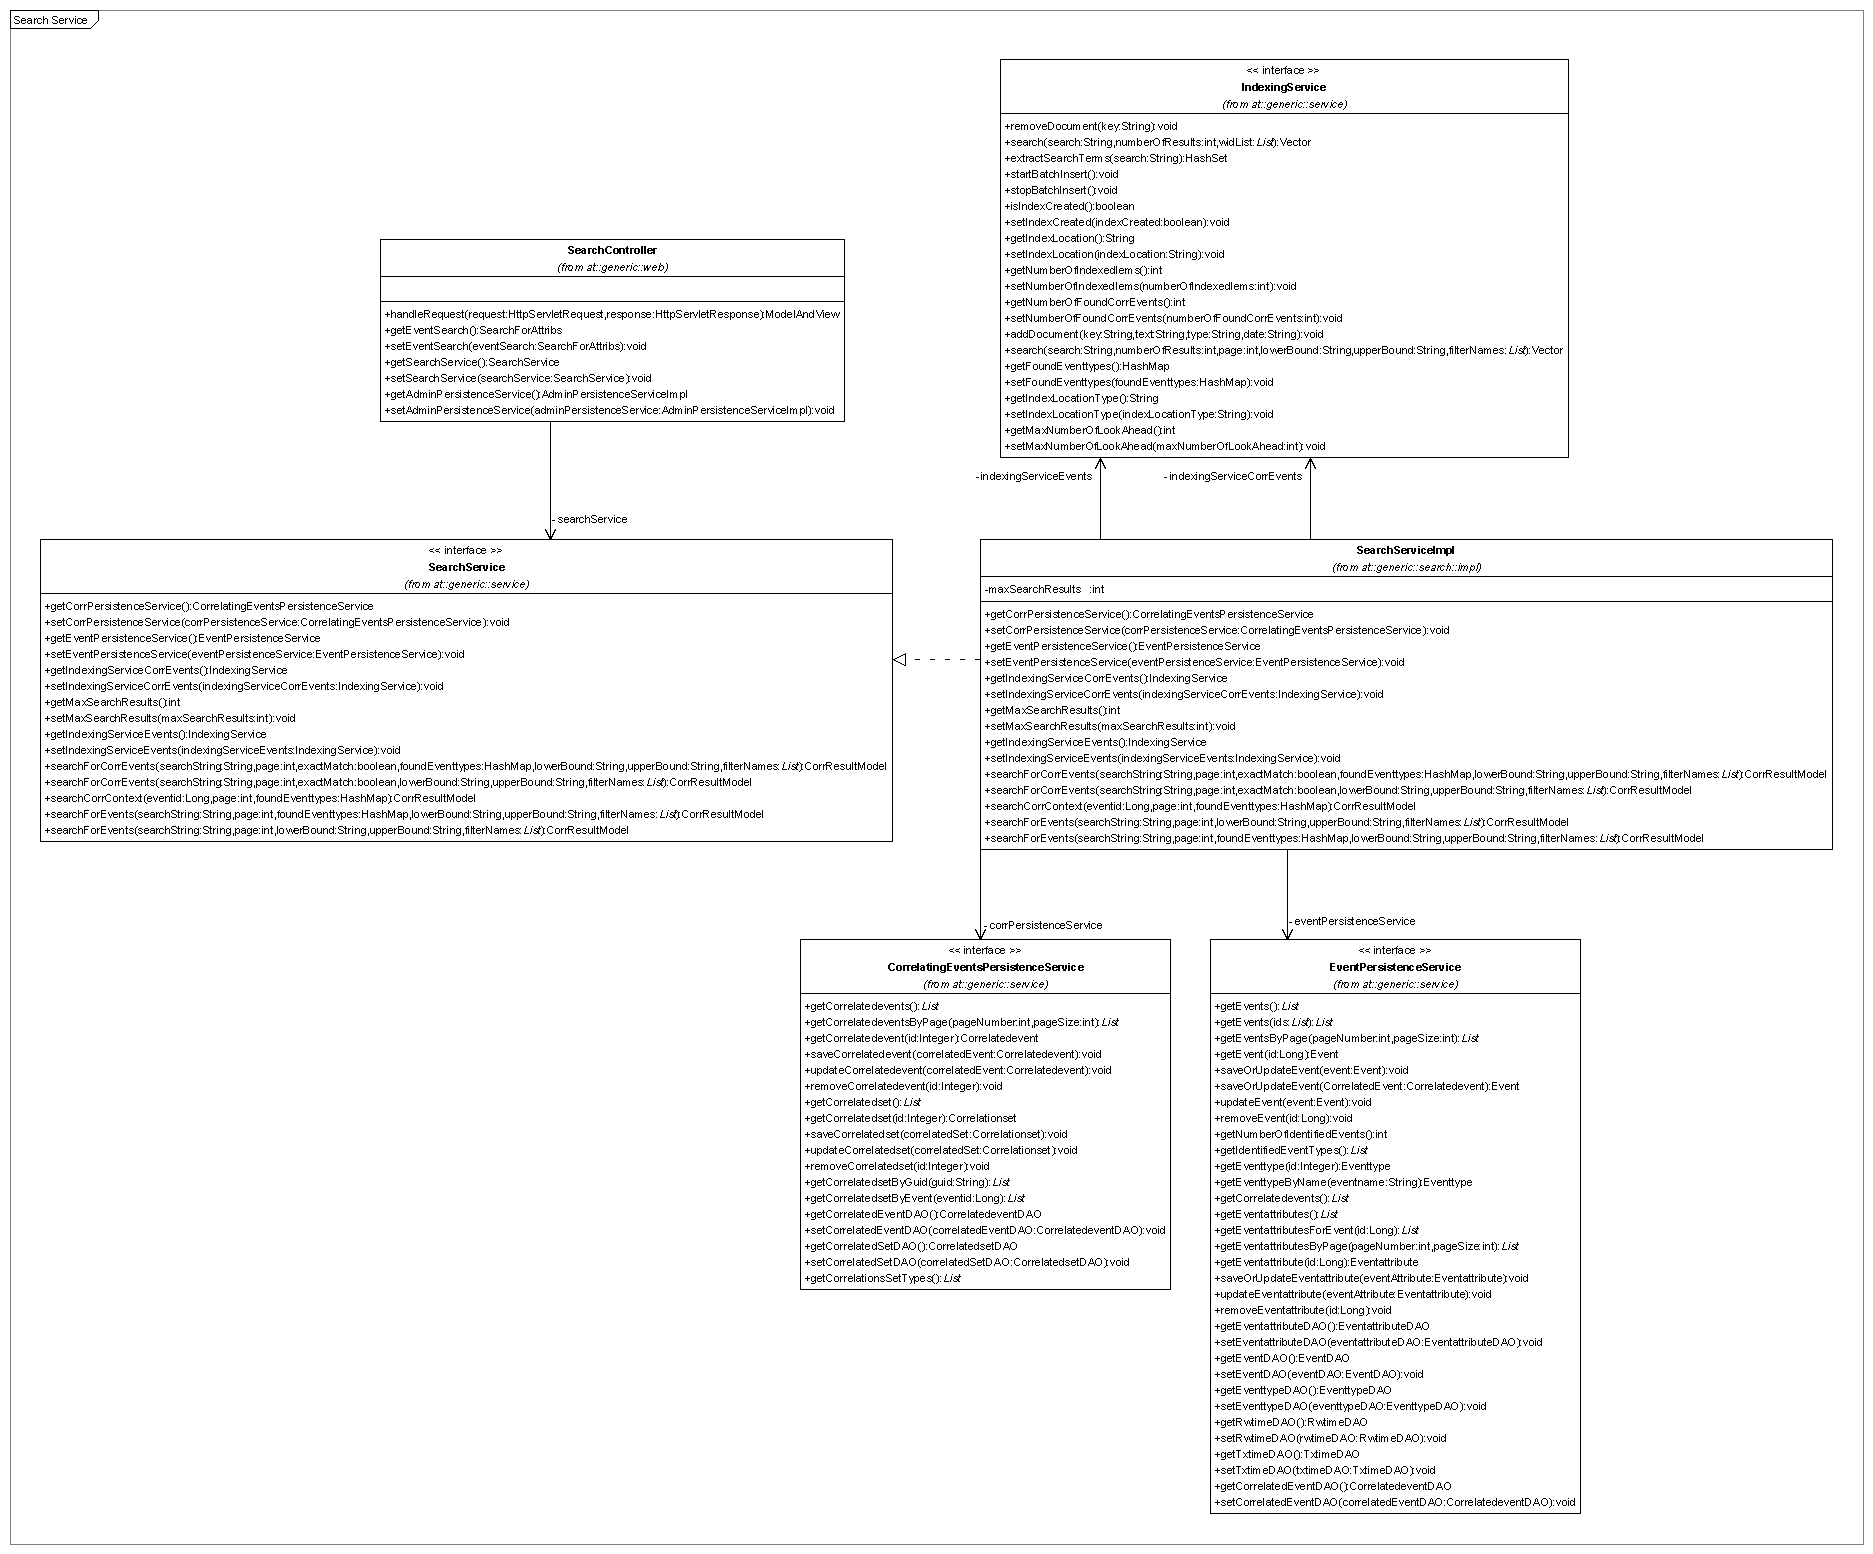
\includegraphics[width=1.2\textwidth]{pics/SearchService.png}
	\caption{Search Service API}             
	\label{fig:Search Service API}
\end{figure}    
%*************************************** 

The SearchService uses the persistence service APIs, but the real search is done inside the IndexingService class as it should encapsulate everything Lucene specific if someone wants to change the underlying indexing technique. This can be done by changing one line in the context configuration as we program against interfaces like everywhere else in this project. The SearchService's job is to manage the creation of the command object that is used by the SearchController to provide the necessary information for the display. The index search is performed by the IndexingService. 
\\\\
Important to note is that Lucene makes extensive use of caching to boost its performance. This is done in a quite unintuitive way so it needs some explanation. Retrieving data from the database, for displaying to the user, is mostly done by using pagination like provided in Event Cloud. The common approach would be to apply the same pagination principle in Lucene for the search results (in Lucene context called hits). The classic way would be to send a query and then retrieve the results according to the page size. This is not done that way with Lucene! Lucene caches these hits and other search related information and therefore it is recommended to requery everytime you switch to another page and display only the hits that are in line for the chosen page. 
\\\\
To be more clear consider following example! You submit a query and Lucene provides 100 results for instance. For page 1 you would show the results from 1 to 10, for page 2 you would requery again and display the results 20 to 30. 
\\\\
Lucene Scorings formula is provided in Figure \ref{fig:LuceneInActionScoring}. Simply spoken the rank score is influenced by following factors:

\begin{itemize}
	\item Documents that contain most or all of the search terms provided in the query are ranked higher.
	\item Matched words that are rare in documents are more valuable than words that are less frequent. 
	\item The scoring is based on the length of a document. A long document is less valuable than a short one.
	\item The occurrence of search terms in a document influences the score. Many matching search terms in a document result in a higher ranking.
\end{itemize}

%***********************
\begin{figure}[!h]                                  
	\centering                                           
	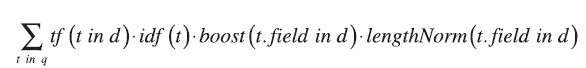
\includegraphics[width=0.8\textwidth]{pics/scoring.jpg}
	\caption{Lucene Scoring \cite{LuceneInAction05}}             
	\label{fig:LuceneInActionScoring}
\end{figure}    
%*************************************** 

%**************************************************************************************
\subsubsection{SearchResultModel}
%**************************************************************************************

%***********************
\begin{figure}[!h]                                  
	\centering                                           
	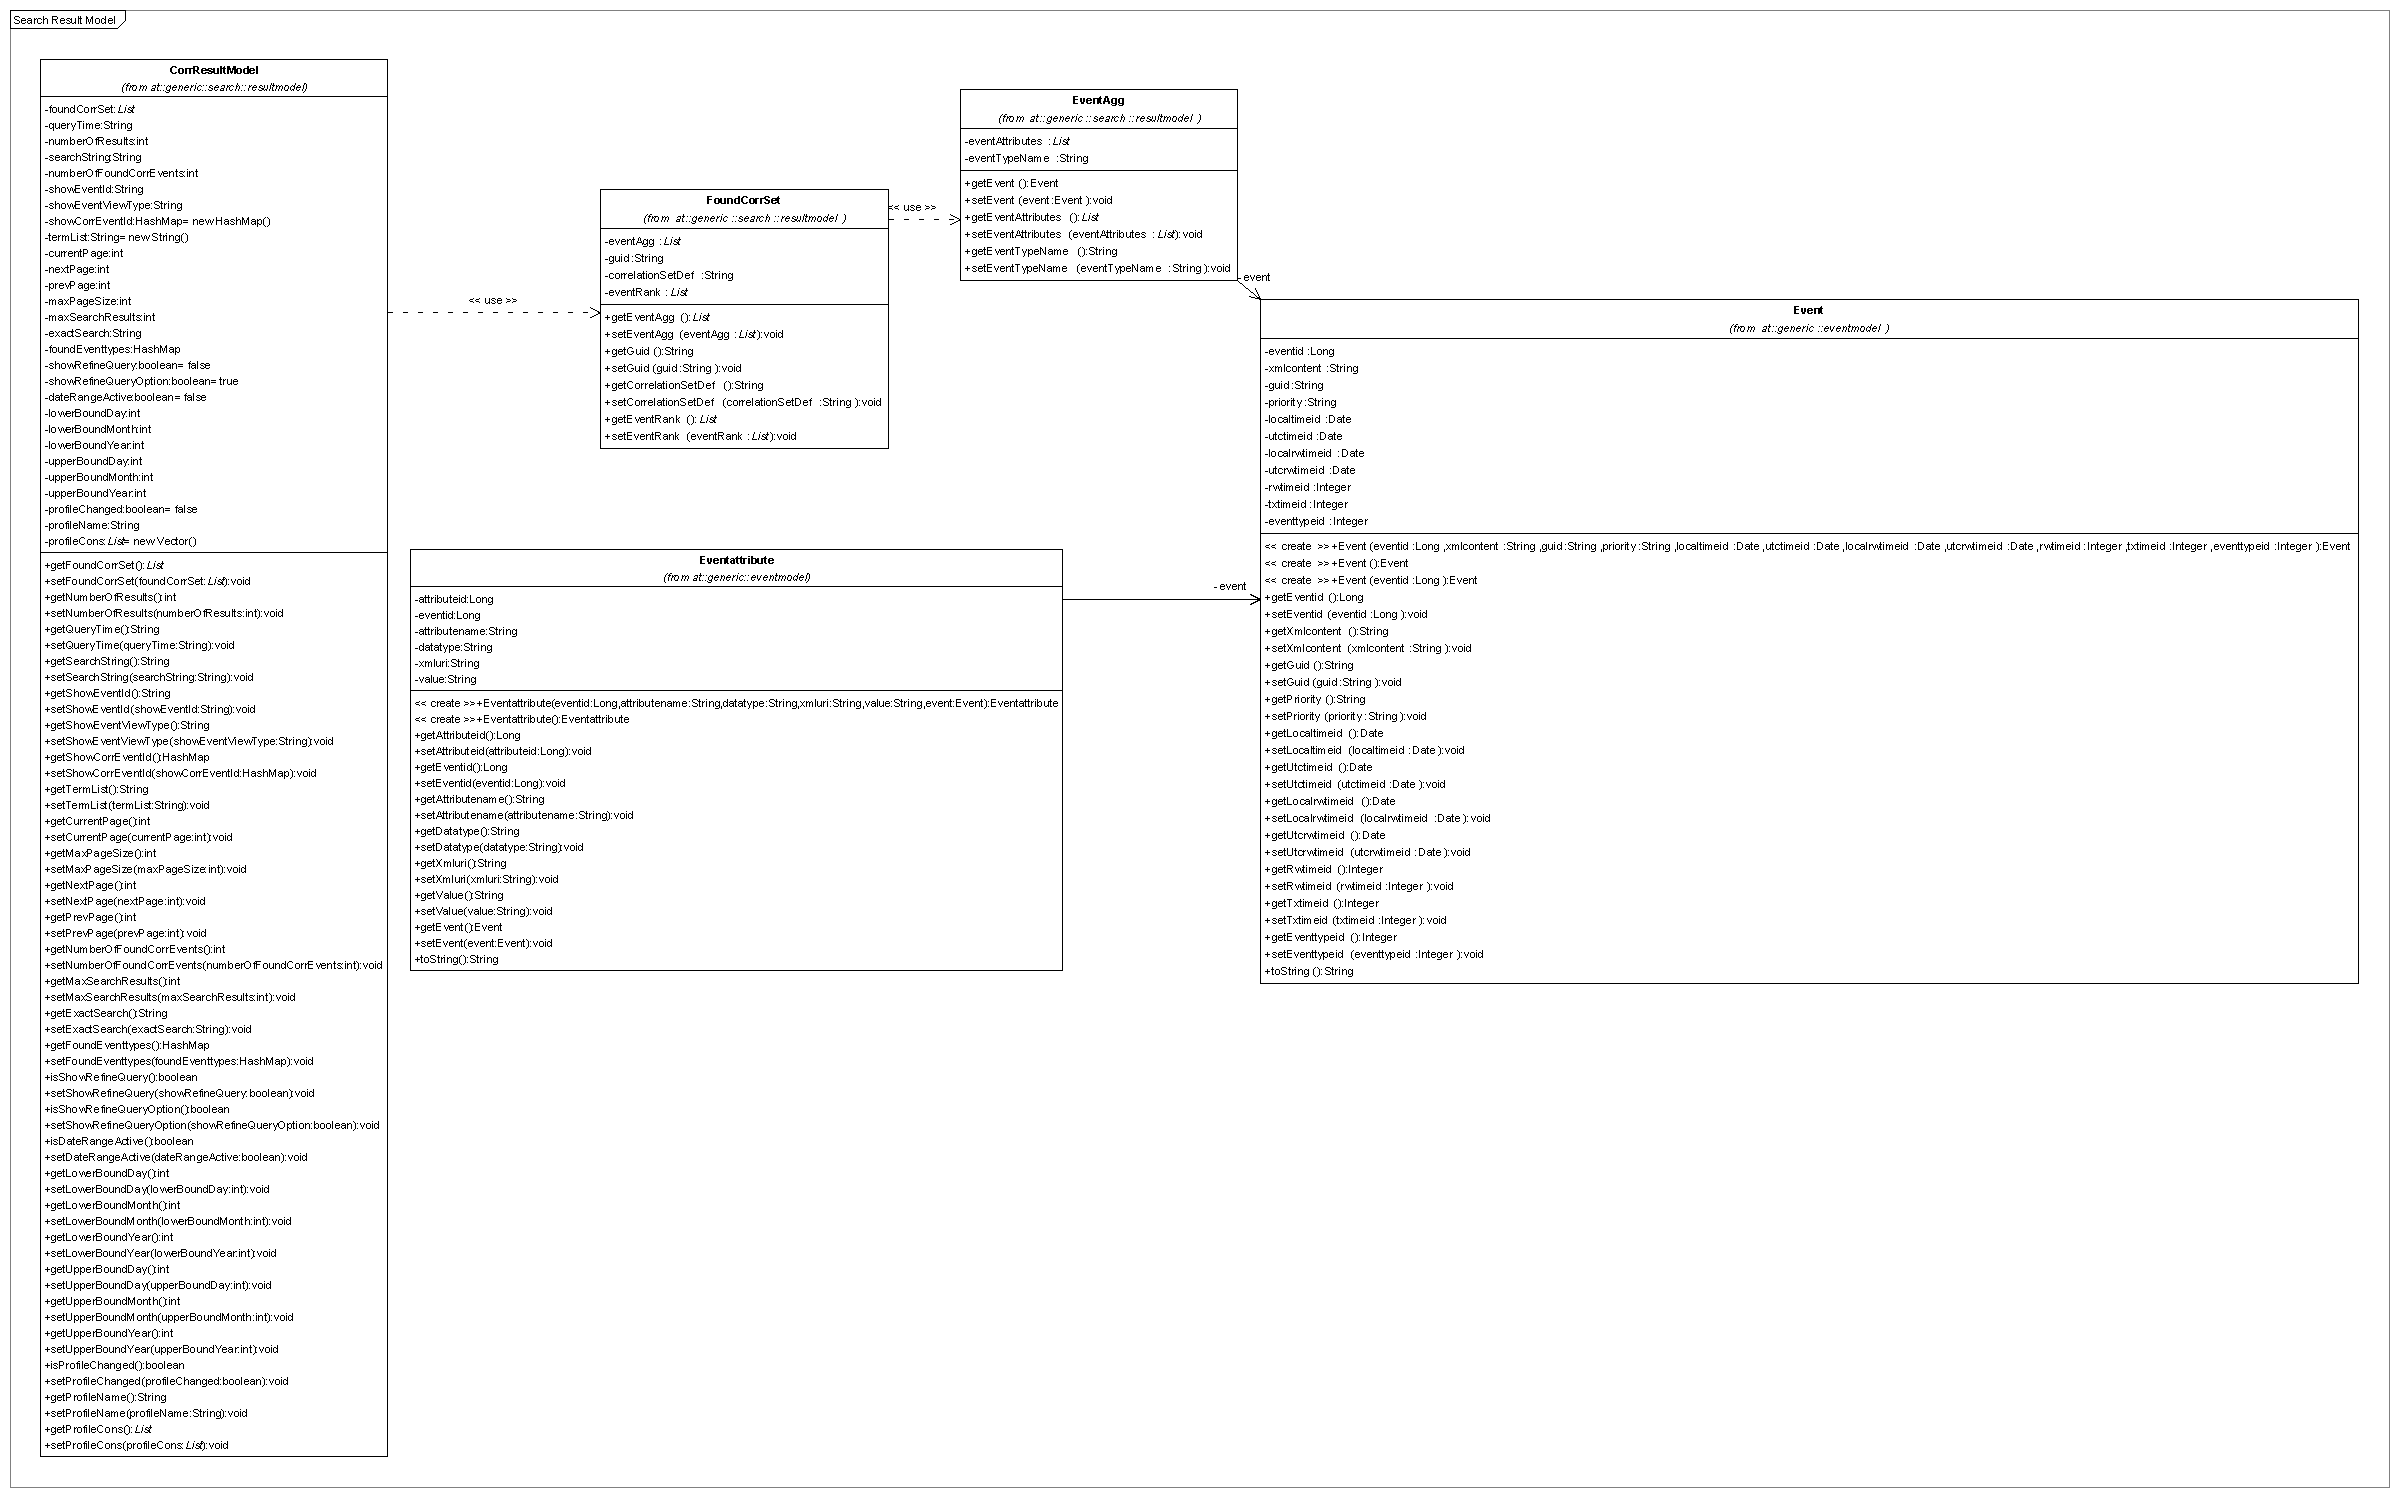
\includegraphics[width=1.2\textwidth]{pics/SearchResultModel.png}
	\caption{Search Service API}             
	\label{fig:SearchServiceAPI}
\end{figure}    
%*************************************** 

The SearchResultModel (Figure \ref{fig:SearchServiceAPI}) is the core command class and is created by the SearchController and the SearchService. This model is used for both Rank 1 and Rank 2 search with the difference that for Rank 1 search there is no FoundCorrSet class. For Rank 1 search the EventAggs are saved into the HashMap instead of FoundCorrSet. Basically the CorrResultModel provides all found correlationsets (FoundCorrSet) and each correlationset has got a collection of events (EventAgg) that have got attached an event object. 
\\\\
The SearchResultModel is also the main point where browser logic, paginiation data and filter information is stored. 

%**************************************************************************************
\subsubsection{Query Syntax}
%**************************************************************************************
Event Cloud is using Lucene's sophisticated query parser to provide a full featured query syntax to allow the creation of complex queries for searching and retrieving events and their correlations. 
\\\\
The formal query grammar definition \cite{LuceneQueryParserAPI}:
\begin{lstlisting} [basicstyle=\ttfamily\fontsize{8}{8}\selectfont]]
Query  ::= ( Clause )*
Clause ::= ["+", "-"] [<TERM> ":"] ( <TERM> | "(" Query ")" )
\end{lstlisting}
A clause can contain either a Term expression or another nested Query. There are two distinctions between terms. There can exist a \textit{single term} like ``hello'' or ``test'' or a term can be a \textit{phrase} like ``hello world'' enclosed by double quotes. It is possible to combine multiple terms with boolean operators \cite{LuceneQueryDescriptionPage}. The predefined Boolean connector configured in Event Cloud for Terms is the OR operator.
\\\\
Some basic query examples are described in the table \ref{tab:LuceneQueryExamples} for getting started.
\\\\
However the QueryParser is capable of much richer functionality like Fuzzy Searches and Proximity Searches. They don't have a big importance in querying but it can be a powerful tool. For example it is possible to create a fuzzy search based on the Levenshtein distance using the tilde ~ symbol plus a proximity number. For example you can search for ``\textit{java~}'' and it will return documents that are similar to java like lava. You can adjust the proximity by adding a value next to the tilde symbol like java~0.8. The default proximity number is 0.5.
\\\\
Another noticeable, but minor feature, is the possibility to define the relevance of search terms in a query with the carrot operator $\wedge$ and a number that specifies the importance of the word. For instance if you search for ``\textit{Paris$\wedge$4 London}'' it will make Paris more relevant than London. The default relevance value is 1.
\\\\
Further details on this topic can be found here \cite{LuceneQueryDescriptionPage}, here \cite{LuceneQueryParserAPI} and here \cite{LuceneInAction05}.

\begin{table}[!hp]
	\begin{tabular}{|p{4cm}|p{8cm}|}
		\hline \textbf{Example} & \textbf{Description} \\
		\hline \textit{Paris} & Query will return events containing ``Paris'' in an Attribute. \\
		\hline  \textit{Paris London} & Query will return events containing either ``Paris'' or ``London'' in an Attribute. \\
		\hline  \textit{Paris OR London} & Query will return events containing either ``Paris'' or ``London'' in an Attribute. \\
		\hline  \textit{Paris AND London} & Query will return events containing ``Paris'' and ``London'' in an Attribute.\\
		\hline  \textit{(Paris OR London) AND Szabolcs} & Query will return events containing ``Paris'' or ``London'' but they must contain ``Szabolcs''.\\
		\hline  \textit{+Paris +London} & Query will return events containing ``Paris'' and ``London'' in an Attribute.\\
		\hline  \textit{+Paris -London} & Query will return events that must contain ``Paris'' and it is not allowed that this event contains ``London'' in an Attribute.\\
		\hline  \textit{+Paris NOT London} & Query will return events that must contain ``Paris'' and it is not allowed that this event contains ``London'' in an Attribute.\\
		\hline  \textit{Par*} & Query will return events containing words that start with ``Par'' - for instance Paris.\\
		\hline 
	\end{tabular}
	\caption{Query Examples}
	\label{tab:LuceneQueryExamples}
\end{table} 

% Verwendete Patterns beschreiben
%	Facade Pattern
% 	Inversion of Control
%	Code injection

% verwendete Technologien beschreiben:
% Tomcat
% Hibernate als OR Mapping
% Datenbank Postgres
% Spring
% MVC Konzept
% Spring MVC
% Lucene



% ETL Prozess
% 	Hibernate als OR Mapping
%		Wie schauen definition files aus
%	Datenbank Postgres

% Indexing 
%	Lucene index structur
%	Verwendung von Lucene als Codebeispiel
%	Caching Themen
%	Darauf eingehen wie man

% Suche
% 	web interface 
%	Spring framework
%	Spring MVC - MVC Konzept im allgemeinen

% Beschreibung der API
%	UML Bilder und beschreiben was was macht

%**************************************************************************************
\subsection{Administration}
%**************************************************************************************

The admin screen (Figure \ref{fig:AdminInterface}) is the main section where users can retrieve information about the running Event Cloud. It provides information about the current transformation process, about the index status. The user can modify the \textit{look ahead} values of the search and the page size for the result list. The \textit{look ahead} value specifies the maximum hit size retrieved by the search. This is necessary to create the event- and correlationtype filters as the search service must be aware of the occurring types in the search hits. The admin interface is also the place for creating and editing profiles.

%***********************
\begin{figure}[!h]                                  
	\centering                                           
	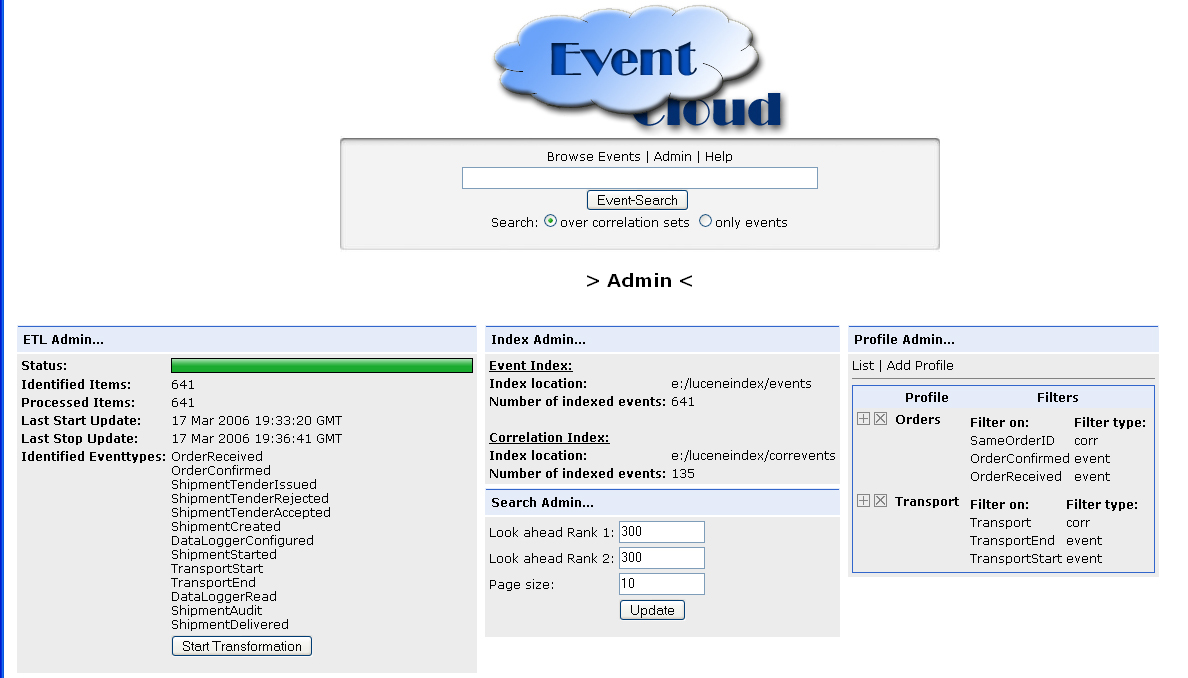
\includegraphics[width=1.0\textwidth]{pics/screenshots/adminScreen.jpg}
	\caption{Admin interface}             
	\label{fig:AdminInterface}
\end{figure}    
%*************************************** 
%**************************************************************************************
\subsubsection{Profiles}
%**************************************************************************************


Event Cloud comes with a set of filters to shrink the size of the found results. As there are specific user groups that are not interested in a wide set of occurred events,  there is a profile editor to shrink the size of occurred events and correlationssets in the results. The user can create various profiles in the administration menue according to his needs (Figure \ref{fig:EditingAProfile} and Figure \ref{fig:AdminInterface}). For example for CRM evaluations you would only need customer specific events or for accounting you would only need order specific events of your result set. These profiles can be applied on the result screen by fading in the options frame on the left side.

%***********************
\begin{figure}[!h]                                  
	\centering                                           
	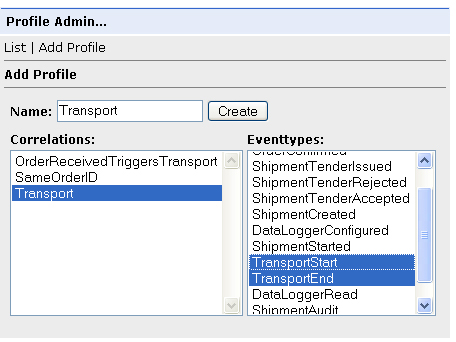
\includegraphics[width=0.7\textwidth]{pics/screenshots/addProfiles.jpg}
	\caption{Editing a profile}             
	\label{fig:EditingAProfile}
\end{figure}    
%*************************************** 


%**************************************************************************************
\newpage
\section{Evolution and Performance Issues}
%**************************************************************************************

EventCloud has evolved over several design implementation steps. The first search implementation was based completely on the relational schema without full text indexing using only the provided Postgresql database indexes (Figure \ref{fig:eventCloudSchema}). These database schema including the indexes has been tested with a script (Listing Figure \ref{lst:TestdataGenerator}) that generates test data (insert statements) with less selective event attributes . For testing 20.000.000 event attributes have been inserted with an event ratio of 1:20 (One event has got 20 attributes).
\\\\
%********************
\begin{figure}[!h]  
	\begin{mytinylisting}
	\begin{verbatim}
	
	#!/bin/bash
	
	targetFile=~/generic/testSplitData.sql
	
	# some vars
	attId=1
	eventId=1
	maxAttribs=20000000
	k=0
	
	# random char vars
	Suites="Paris Wien Munich Stockholm Budapest Rom Barcelona 
			Madrid Hamburg Helsinki London Oxford Rotterdam Amsterdam 
			Berlin Belgrad Klagenfurt Graz Bern Lyon"
	
	suite=($Suites)
	
	num_suites=${#suite[*]}        # Count how many elements.
	
	touch $targetFile
	
	echo "INSERT INTO events (eventid) VALUES ("$eventId");"  >> $targetFile
	
	# das selbe wie for (eventId=1; eventId < maxAttribs; eventId++)
	while [ $attId -le $maxAttribs ]
	do

        if [ $k -eq 20 ]; then
                k=0
                eventId=$((eventId+1))
                echo "INSERT INTO events (eventid) VALUES ("$eventId");"  >> $targetFile
        else
                k=$((k+1))
        fi

        PASS=${suite[$((RANDOM%num_suites))]}

        echo "INSERT INTO eventattributes (eventid, attributeid, attributename, value) 
        				VALUES ("$eventId","$attId", '"$PASS"' , '"$PASS"');" >> $targetFile

        attId=$((attId+1))
	done	
	\end{verbatim}
    \end{mytinylisting}
	\caption{Testdata generator}             
	\label{lst:TestdataGenerator}
\end{figure} 
%********************

The insertion of the testdata into database takes quite long as there are enormous hard disk accesses going on (Listing Figure \ref{lst:CreatingAndInsertingTestData}). The test systems specifications are:

\begin{itemize}
	\item Athlon XP 1800
	\item 512MB Ram
	\item Gentoo Linux 2.6.9-gentoo-r9
	\item Postgresql 8.0.4
\end{itemize}

%********************
\begin{figure}[!h]  
	\begin{mytinylisting}
	\begin{verbatim}
	time ./createSplitTestData.sh &
	
	real    74m49.518s
	user    57m2.370s
	sys     10m12.932s
	
	
	time cat /home/szabolcs/generic/testSplitData.sql | psql genericsplit &
	
	real    906m42.487s
	user    35m54.828s
	sys     16m0.516s
	\end{verbatim}
    \end{mytinylisting}
	\caption{Creating and inserting test data}             
	\label{lst:CreatingAndInsertingTestData}
\end{figure} 
%********************

A simple database query for retrieving eventattributes according to a given value takes quite long as there is a huge amount of data to be retrieved and displayed (Listing Figure \ref{lst:RetrievingAnAttribute}). The solution is to create a pagination on displaying such huge number of datasets (Listing Figure \ref{lst:RetrievingAnAttributeWithPagination}). This shows that the query itself is extremly fast but displaying or retrieving the datasets can take very long. The workaround is to apply pagination on the query.

%********************
\begin{figure}[!h]  
	\begin{mytinylisting}
	\begin{verbatim}
	time echo "select * from eventattributes where value ='Rom'" | psql genericsplit
	
	real    7m47.986s
	user    0m5.049s
	sys     0m3.089s
	\end{verbatim}
    \end{mytinylisting}
	\caption{Retrieving an attribute}             
	\label{lst:RetrievingAnAttribute}
\end{figure} 
%********************

%********************
\begin{figure}[!h]  
	\begin{mytinylisting}
	\begin{verbatim}
	time echo "select * from eventattributes where value ='Rom' limit (300) offset 0" | psql genericsplit
	
	real    0m0.392s
	user    0m0.006s
	sys     0m0.007s
	\end{verbatim}
    \end{mytinylisting}
	\caption{Retrieving an attribute using pagination}             
	\label{lst:RetrievingAnAttributeWithPagination}
\end{figure} 
%********************

The tests showed that PostgreSql and the database schema can perform in a fast way. Two problems emerged using the relational schema for the Rank 1 search. The first is that a sophisticated query parser has to be implemented. A rudimentary parser has been created for the first use. The second one is that using AND connections of search terms is a common way of searching data, but applying \textit{AND} connections with this schema would result in an extremly bad peformance behaviour. This is because searching for several event attributes would require to create a carthesian product that creates a huge overhead of datasets (Listing Figure \ref{lst:CarthesianProduct}).

%********************
\begin{figure}[!h]  
	\begin{mytinylisting}
	\begin{verbatim}
	time echo "select distinct a.* from eventattributes a, eventattributes b  where a.eventid = b.eventid 
		and  a.value = 'Rom' and b.value = 'Paris' limit(10)" | psql genericsplit

	real    10m40.541s
	user    0m0.005s
	sys     0m0.007s

	\end{verbatim}
    \end{mytinylisting}
	\caption{Carthesian product}             
	\label{lst:CarthesianProduct}
\end{figure} 
%********************

The main problem using this schema as the primary event search was the Rank 2 search that does not allow to search through the datasets in segments (by pages) like it would be possible with Rank 1. Executing a query with the Rank 1 search implementation would create a hits on 10.000 events for instance. These hits could be retrieved in a fast performing way using pagination apart from the carthesian product issue. This would not work out for the Rank 2 search as you would need every matching eventattributes to find and evaluate the causal relationships. This is because the search query is not restrained on one event. It has to consider every event that belongs to a correlation. 
\\\\
The Figure \ref{fig:Rank2problems} shows how the search would work using the database schema as the search infrastructure. The first step is to apply the query to eventattributes which results in a huge set of datasets that matched that query. The huge sets are common, as event attributes are less selective. The next step would be to retrieve the correlation sets for every found event and then recheck the processess in the relating events. This way would perform very poor.
\\\\
The solution was to use a full text indexing technology for the search that resulted in Event Cloud's current architecture. This approach is a top down way as attributes of events are directly related to correlations.

%***********************
\begin{figure}[!h]                                  
	\centering                                           
	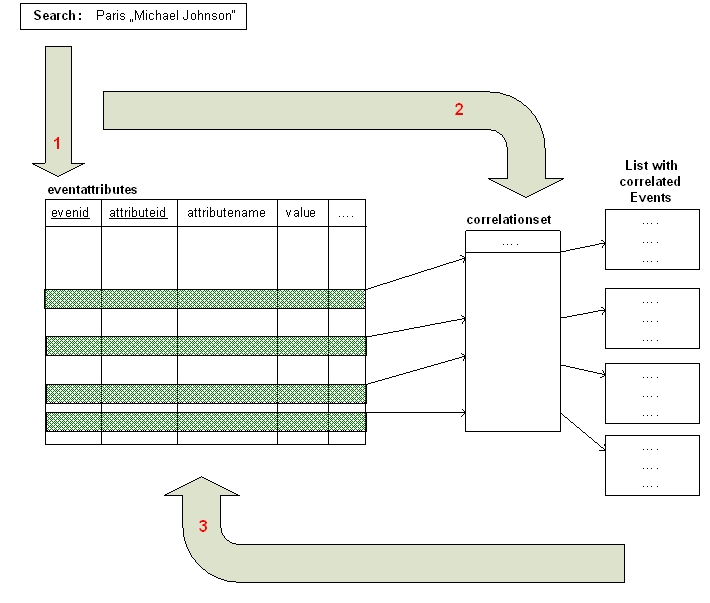
\includegraphics[width=1.0\textwidth]{pics/FirstApproach.jpg}
	\caption{Rank 2 problems}             
	\label{fig:Rank2problems}
\end{figure}    
%*************************************** 

%**************************************************************************************
\subsection{Simulation}
%**************************************************************************************

The test data for Event Cloud has been generated using Intime. The event definitions are created either by hand writing XML files or by using Intime's graphical editor. The whole event data is based on a logistics scenario written in cooperation with Roland Vecera. Details about the simulation process and the story itself is provided in the Appendix.

%**************************************************************************************
\newpage
\section{Conclusion}
%**************************************************************************************

Event Cloud has shown that it is possible to create an easy-to-use application to manage the access to the huge amounts of events in an efficient way. However there are some open issues that must be solved in further projects. The Rank 3 search type is undisputable one of the essential features that is missing in the current version of Event Cloud. The scaleability of Lucene's index is limited to the physical borders of one machine. As there would be billions of events stored in the indexes there is physical limit of one machine. There is already discussion going on that Lucene should support clustering to distribute its indexes over several machines in order to scale up to large requirements. This could be done by distributing the indexes over serveral machines and let one machine control the retrieval process. Currently there is no concrete plan to implement such a feature.

%**************************************************************************************
\newpage
\section{Acknowledgements}
\textbf{TODO}
%**************************************************************************************

%**************************************************************************************
\newpage
\section{Appendix}
%**************************************************************************************
%**************************************************************************************
\newpage
\begin{landscape}
\subsection{Data Access Diagram}
%**************************************************************************************
%***********************
\begin{figure}[!h]                                  
	\centering                                           
	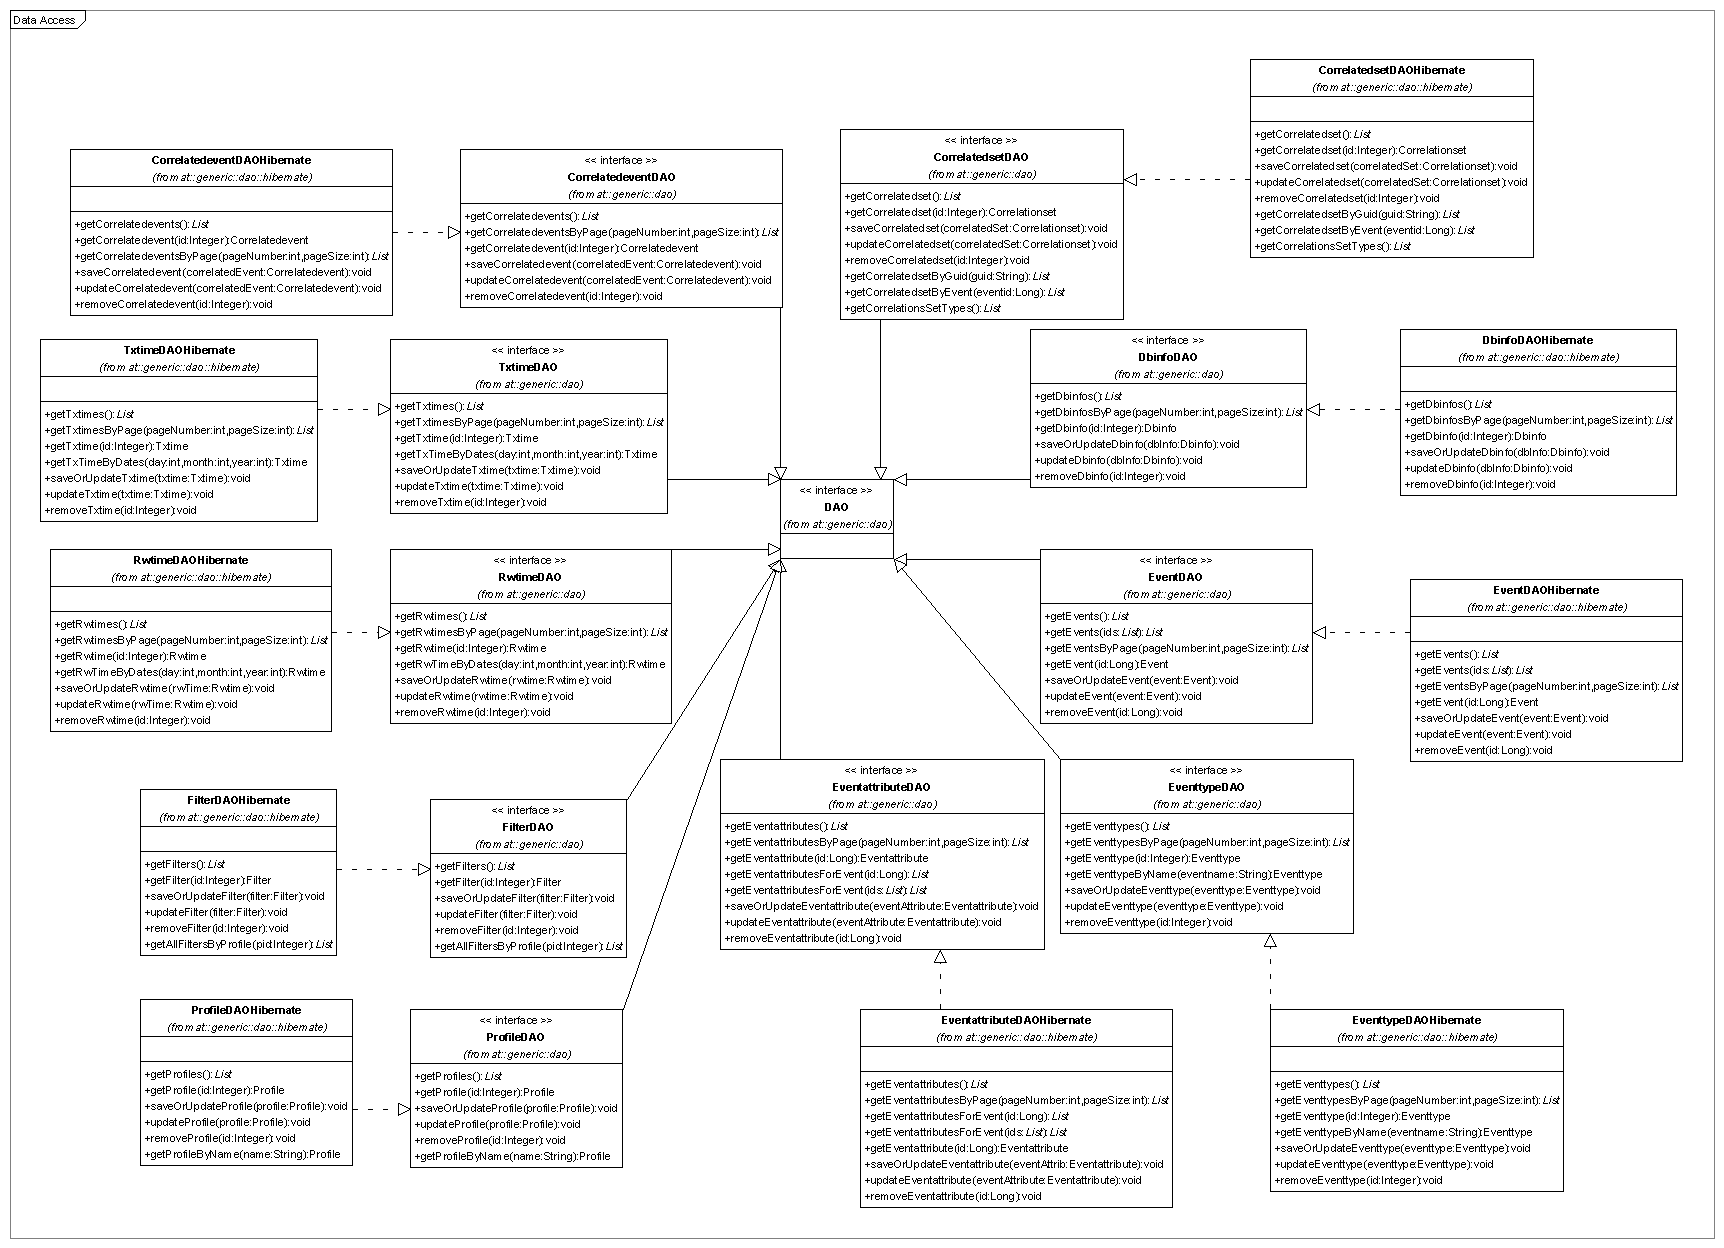
\includegraphics[width=1.1\textwidth]{pics/DataAccess.png}
	\caption{Data Access}             
	\label{fig:GeneralDataAccess}
\end{figure}            
%*********************** 
\end{landscape}

%**************************************************************************************
% TITLE
%**************************************************************************************
%**************************************************************************************
\subsection{Simulation Stories - Introduction}
%**************************************************************************************

%**************************************************************************************
\subsubsection{MediTransCare - About the company}
%**************************************************************************************
MediTransCare is a company specialized on medical goods settled in Vienna. Its custom-ers are distributed all over Europe. The emphasis of the enterprise is on secure and in-time delivery of medical goods. For this purpose MediTransCare owns a distribution and storage network across Europe.
\\\\
In the field of "medical logistics" it is vital not to break the cold chain of pharmaceuticals or to overrun the expiry date. During transportation and temporary storage pharmaceuti-cals can be exposed to heavy surrounding conditions that can damage the goods. Fur-thermore the products have to be secured against theft (abuse).
\\\\
The requirement in the medical supply field grows more than ever and the requirements on logistics in reference to an economic distribution forms here the emphasis.  Many cus-tomers appreciate a just-in-time delivery whereby special attention is set on that no bot-tlenecks or over-capacities arise locally.
\\\\
The company makes extensive use of IT systems that can identify and predict future needs and demands of its customers. It can create profiles out of behaviour patterns and seasonal empirical values. Thus it can recognize automatically that a shortage on sup-plies is going to become apparent and deploy counter measures to avoid such situations. It can order buffer deliveries, store and secure them and in case of demand deliver the products within hours to its customers.
\\\\
MediTransCare selects among reliable carriers based on economical aspects to deliver their products.  The carriers have to be able to accomplish the assignment within the specified conditions (e.g. special cooling, delivery date). Together with the carriers MediTransCare works out an exact delivery plan to ensure that the delivery arrives in time.
\\\\
The buffer of pharmaceuticals is secured through a network of local storage depots that can assure the high standards required by storing pharmaceuticals. Local carriers can de-liver the ordered goods within hours to the customers.
\\\\
Basically MediTransCare is able to deliver products in Europe within 4 to 7 days from one depot storage to another one. The means of transport are either by truck or by cargo planes depending on the requirements.
\\\\
The whole delivery process is under constant surveillance to be able to react on problems like quality, delivery delays or loss.

%**********************
\begin{figure}[!h]                               
	\centering                                           
	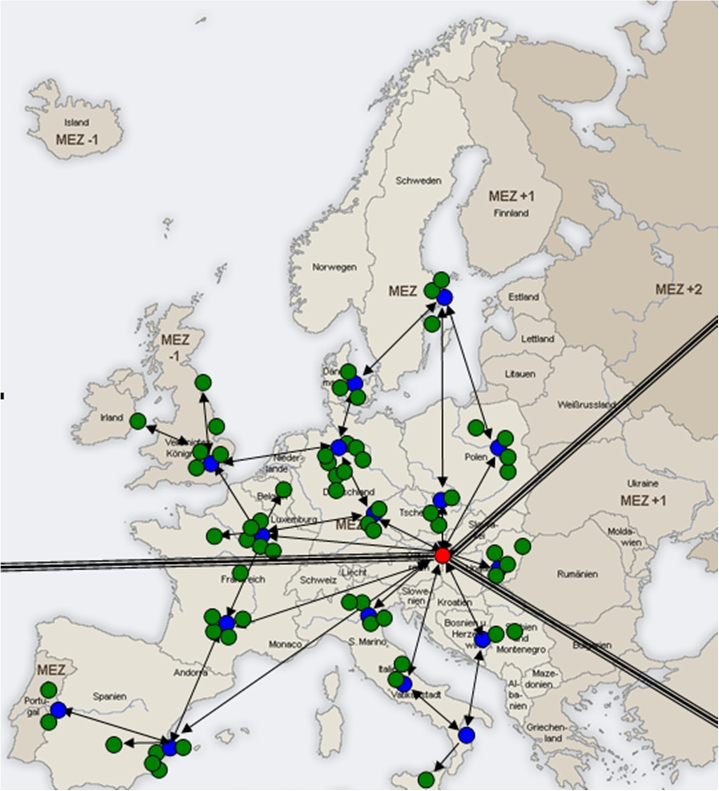
\includegraphics[width=1\textwidth]{pics/europeMap.jpg}
	\caption{MediTransCare's transportation network}             
	\label{fig:MediTransCaretransportationnetwork}
\end{figure}  
%**********************

%**************************************************************************************
\subsubsection{The delivery process}
%**************************************************************************************
The basic phases during a delivery process look like as follows:

\begin{itemize}
	\item Load Planning 
	\item Load Tendering
	\item Carrier Dispatch and Load
	\item InTransit - Track and Trace
\end{itemize}
In the following sections the process of a delivery between local storage depots will be explained. This process starting from an incoming order to the final delivery at the de-sired destination is described in the following sections.

%**************************************************************************************
\subsubsection{The Offer}
%**************************************************************************************
A local storage depot requests a delivery of one or more products if the stock level sinks under a predefined threshold, a higher demand is expected or you get a big order from a customer. Usually this is done through an IT system. The order will be handed over to a proper coordinator (Transportation Planner) who is responsible for planning and dispatch-ing outgoing supplies. He will handle the order further on.

%**************************************************************************************
\subsubsection{Load Tendering}
%**************************************************************************************
The Transportation Planner forwards the offer with its cargo characteristics and the gen-eral conditions to a pool of carriers.
\\\\
For almost all deliveries going out from MediTransCare a cooling is required for the cargo, because almost every medical good has to stay between a temperature-interval in order to ensure the quality.
\\\\
It also can happen that a transport needs two different temperature zones for pharma-ceutics that require a different cooling temperature. This would require special equipment to create two different climate chambers. These requirements have to be announced to all carriers so that they can prepare their equipment or to check their utilization.
\\\\
The contacted carriers have to reply within a specific time period if they want to accept or reject the offer.
%**************************************************************************************
\subsubsection{Load Planning}
%**************************************************************************************
Right after the decision has been made which carrier will perform the delivery, a detailed plan is developed together with the selected carrier that defines exactly how the trans-port will be executed.
\\\\
This plan contains the sections with the stops and reloads on the way to the target desti-nation. For example a cargo from Vienna to Madrid would take the route from Vienna to Munich and then from Munich to Madrid. Over night the cargo has to be stored in the de-pot in Munich.
\\\\
To be able to control and track the transport you need more information besides delivery dates. There is a definition for buffer times for each section on the route. With these times it is possible to identify imminent delays. 

%**************************************************************************************
\subsubsection{Carrier Dispatch and Load}
%**************************************************************************************
The medical supplies are usually packed between polystyrene boxes layered up in boxes. If necessary the cargo is cooled with dry ice during packaging. 

%**********************
\begin{figure}[!h]                               
	\centering                                           
	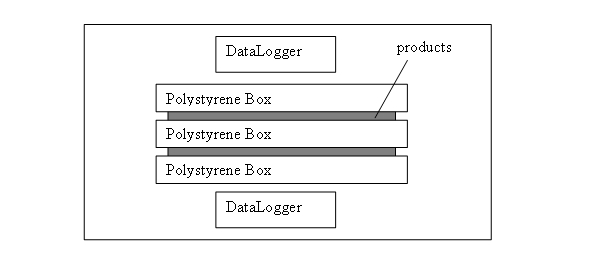
\includegraphics[width=1\textwidth]{pics/transportBox.jpg}
	\caption{Polystyrene package}             
	\label{fig:Polystyrene package}
\end{figure}  
%**********************

Multiple dataloggers are packed between the stacked boxes to measure every 60 minutes (standard value) the temperature to achieve meaningful results. With these measure-ments you can ensure the quality of the products after a transportation.
\\\\
Dataloggers are programmed with following data before they are packed into the cargo:

\begin{itemize}
	\item Logger Id
	\item Order Id
	\item Destination
	\item Min-Max temperature threshold
	\item How often should the datalogger measure the temperature (Standard: every 60min)
	\item Person who has programmed the datalogger
\end{itemize}

A datalogger has a maximal capacity of 200 measurements which means that the trans-port duration is limited if you want to ensure the product's quality.

%**************************************************************************************
\subsubsection{InTransit - Track and Trace}
%**************************************************************************************
The cargo is handed over to the contracted carrier at the beginning. 
\\\\
The transport goes usually over several stages where the supplies have to be reloaded. Like: 
\\\\
The transport goes over several stations by truck or by train to the desired destination.
The carrier reloads the shipment on a cargo plane. Arrived at the flight destination the cargo is reloaded again onto a local carrier truck that brings the shipment to the destina-tion.
\\\\
At the end of each section the delivery is checked. On one hand the correctness of the quantity is controlled and on the other hand the quality of the products. The delivery has to be in the planned delivery time.
\\\\
The quality control is done by examining the dataloggers to ensure that the last stage went alright and the products haven't been exposed to illegal temperatures.

%**************************************************************************************
\subsubsection{Acceptance of Shipment}
%**************************************************************************************
When the product arrived at the destination a storage depot staffmember examines the cargo. The shipment has to be complete and visually alright. Afterwards the dataloggers are taken out for an analysis (e.g. measured temperatures are read out). 
\\\\
If the measurements are valid too and the shipment was delivered in time than the transport is booked as a success and is completed.

%**************************************************************************************
\subsubsection{Process-events}
%**************************************************************************************
In this section the events are described that are generated during a process flow.
\\\\
\textbf{OrderReceived} (OrderId, DateTime, DeliveryDate, Destination, ProductCollection)\\
This event occurs if a new order has been generated.
\begin{mytinylisting}
	\begin{verbatim}
<OrderReceived>
		<OrderId>14765</OrderId>
		<DateTime>2005-10-31T11:31:02</DateTime>
		<DeliveryDate>2005-11-12T06:00:00</DeliveryDate>
		<Destination>Madrid</Destination>
		<ProductCollection>
			<Product>		
    	<ProductId>Arzeutic</ProductId>
	<Amount>700</Amount>
</Product>	
		</ProductCollection>
</OrderReceived>
\end{verbatim}
\end{mytinylisting}


\textbf{OrderConfirmed} (OrderId, DateTime)\\
This event occurs if an offer has been confirmed.
\begin{mytinylisting}
\begin{verbatim}
<OrderConfirmed>
		<OrderId>14765</OrderId>
		<DateTime>2005-10-31T13:45:17</DateTime>
</OrderConfirmed>
\end{verbatim}
\end{mytinylisting}


\textbf{ShipmentTenderIssued} (OrderId, DateTime, FurtherInfo) \\
The order including conditions and constraints is sent to a pool of carriers.
\begin{mytinylisting}
\begin{verbatim}
<ShipmentTenderIssued>
	<OrderId>14765</OrderId>
	<DateTime>2005-10-31T14:12:54</DateTime>
	<FurtherInfo>
		<ShipmentInfo>		
    	<From>Vienna</From>
	<To>Madrid</To>
	<DeliveryDate>2005-11-12T06:00:00</DeliveryDate>
	<TransportType>Truck</TransportType>
	<Price>2500</Price>
	<MinTemp>3</MinTemp>
	<MaxTemp>8</MaxTemp>
</ShipmentInfo>
	</FurtherInfo>
</ShipmentTenderIssued>	
\end{verbatim}
\end{mytinylisting}


\textbf{ShipmentTenderAccepted} (OrderId, CarrierId, DateTime)\\
The carrier accepts the tender.
\begin{mytinylisting}
\begin{verbatim}
<OrderConfirmed>
	<OrderId>14765</OrderId>
	<CarrierId>433</CarrierId>
	<DateTime>2005-10-31T13:45:17</DateTime>
</OrderConfirmed>	

\end{verbatim}
\end{mytinylisting}


\textbf{ShipmentTenderRejected} (OrderId, CarrierId, DateTime)\\
The carrier rejects the tendered transport under the given conditions.
\begin{mytinylisting}
\begin{verbatim}
<ShipmentTenderRejected> 
		<OrderId>14765</OrderId>
		<CarrierId>532</CarrierId>
		<DateTime>2005-10-31T15:12:21</DateTime>
</ShipmentTenderRejected>
\end{verbatim}
\end{mytinylisting}


\textbf{ShipmentCreated} (OrderId, TransportId, CarrierId, DateTime, DatePlannedShipped, DatePlannedDelivered, DateEarlyBuffered, DateLateBuffered, LocationFrom, LocationTo, Miles, PlannedFreightCosts, TransportType)\\
The shipment specifications worked out together with the carrier. These values mark a successful delivery and they are controlled by the system. A shipment can contain more than one stage ("TransportInfo", TransportStart-TransportEnd).
\begin{mytinylisting}
\begin{verbatim}
<ShipmentCreated> 
	<OrderId>14765</OrderId>
	<DateTime>2005-10-31T15:45:25</DateTime>
      <Transport>
<TransportInfo>
      <TransportId>42322</TransportId>
	<CarrierId>433</CarrierId>
	<DatePlannedShipped>2005-11-07T08:15:00</DatePlannedShipped>
	<DatePlannedDelivered>2005-11-7T17:00:00</DatePlannedDelivered>
	<DateEarlyBuffered>2005-11-06T16:00:00</DateEarlyBuffered>
	<DateLateBuffered>2005-11-08T06:00:00</DateLateBuffered>
	<LocationFrom>Vienna</LocationFrom>
	<LocationTo>Munich</LocationTo>
	<Miles>422</Miles>
	<PlannedFreightCosts>690</PlannedFreightCosts>
	<TransportType>Truck</TransportType>
</TransportInfo>
<TransportInfo>
      <TransportId>42323</TransportId>
	<CarrierId>433</CarrierId>
	<DatePlannedShipped>2005-11-08T14:00:00</DatePlannedShipped>
	<DatePlannedDelivered>2005-11-0T17:00:00</DatePlannedDelivered>
	<DateEarlyBuffered>2005-11-07T17:00:00</DateEarlyBuffered>
	<DateLateBuffered>2005-11-12T06:00:00</DateLateBuffered>
	<LocationFrom>Munich</LocationFrom>
	<LocationTo>Madrid</LocationTo>
	<Miles>1810</Miles>
	<PlannedFreightCosts>690</PlannedFreightCosts>
	<TransportType>Truck</TransportType>
</TransportInfo>
      </Transport>
</ShipmentCreated>
\end{verbatim}
\end{mytinylisting}


\textbf{DataLoggerConfigured} (OrderId, LoggerId, DateTime, Staffmember, MinTemp, MaxTemp, SenseInterval, Destination)\\
Datalogger settings for shipment monitoring.
\begin{mytinylisting}
\begin{verbatim}
<DataLoggerConfigured>
	<OrderId>14765</OrderId>
	<LoggerId>977</LoggerId>
	<DateTime>2005-11-02T16:01:44</DateTime>
	<Staffmember>Michael Johnson</Staffmember>
	<MinTemp>3</MinTemp>
	<MaxTemp>8</MaxTemp>
	<SenseInterval>60</SenseInterval>
	<Destination>Madrid</Destination>
</DataLoggerConfigured>

\end{verbatim}
\end{mytinylisting}


\textbf{ShipmentStarted} (OrderId, DateTime) \\
Signals the start of a shipment.
\begin{mytinylisting}
\begin{verbatim}
<ShipmentStarted>
	<OrderId>14765</OrderId>
	<DateTime>2005-11-07T08:15:11</DateTime>
</ShipmentStarted>
\end{verbatim}
\end{mytinylisting}


\textbf{TransportStart} (OrderId, TransportId, DateTime, Location, CarrierId)\\
Signals the start of a transport (stage of a shipment).
\begin{mytinylisting}
\begin{verbatim}
<TransportStart>
	<OrderId>14765</OrderId>
	<TransportId>42322</TransportId>
	<DateTime>2005-11-07T08:20:41</DateTime>
	<Location>Vienna</Location> 
	<CarrierId>433</CarrierId>
</TransportStart>
\end{verbatim}
\end{mytinylisting}


\textbf{ShipmentExpedited} (OrderId, TransportId, DateTime, DatePlannedShipped, DatePlannedDelivered, DateEarlyBuffered, DateLateBuffered, LocationFrom, LocationTo, Miles, PlannedFreightCosts, TransportType)\\
It can occur that the route of a transport has to be changed. A new planning has to be done. This event shows that a transport has been cancelled or changed.
\begin{mytinylisting}
\begin{verbatim}
<ShipmentExpedited> 
	<OrderId>14765</OrderId>
	<DateTime>2005-10-31T15:45:25</DateTime>
      <Transport>
   <TransportInfo>
      <TransportId>42322</TransportId>
	<CarrierId>433</CarrierId>
	<DatePlannedShipped>2005-11-07T08:15:00</DatePlannedShipped>
	<DatePlannedDelivered>2005-11-7T17:00:00</DatePlannedDelivered>
	<DateEarlyBuffered>2005-11-06T16:00:00</DateEarlyBuffered>
	<DateLateBuffered>2005-11-08T06:00:00</DateLateBuffered>
	<LocationFrom>Vienna</LocationFrom>
	<LocationTo>Munich</LocationTo>
	<Miles>422</Miles>
	<PlannedFreightCosts>690</PlannedFreightCosts>
	<TransportType>Truck</TransportType>
         </TransportInfo>
      </Transport>
</ShipmentExpedited>
\end{verbatim}
\end{mytinylisting}


\textbf{TransportEnd} (OrderId, TransportId, DateTime, DatePlannedShipped, DatePlannedDelivered, DateEarlyBuffered, DateLateBuffered, LocationFrom, LocationTo, Miles, PlannedFreightCosts, TransportType)\\
It can occur that the route of a transport has to be changed. A new planning has to be done. This event shows that a transport has been cancelled or changed.
\begin{mytinylisting}
\begin{verbatim}
<ShipmentExpedited> 
	<OrderId>14765</OrderId>
	<DateTime>2005-10-31T15:45:25</DateTime>
      <Transport>
   <TransportInfo>
      <TransportId>42322</TransportId>
	<CarrierId>433</CarrierId>
	<DatePlannedShipped>2005-11-07T08:15:00</DatePlannedShipped>
	<DatePlannedDelivered>2005-11-7T17:00:00</DatePlannedDelivered>
	<DateEarlyBuffered>2005-11-06T16:00:00</DateEarlyBuffered>
	<DateLateBuffered>2005-11-08T06:00:00</DateLateBuffered>
	<LocationFrom>Vienna</LocationFrom>
	<LocationTo>Munich</LocationTo>
	<Miles>422</Miles>
	<PlannedFreightCosts>690</PlannedFreightCosts>
	<TransportType>Truck</TransportType>
         </TransportInfo>
      </Transport>
</ShipmentExpedited>
\end{verbatim}
\end{mytinylisting}

\textbf{TransportEnd} (OrderId, TransportId, DateTime, Location, CarrierId)\\
The end of a transport.
\begin{mytinylisting}
\begin{verbatim}
<TransportStart>
	<OrderId>14765</OrderId>
	<TransportId>42322</TransportId>
	<DateTime>2005-11-07T16:07:07</DateTime>
	<Location>Munich</Location> 
</TransportStart>
\end{verbatim}
\end{mytinylisting}


\textbf{DataLoggerRead} (OrderId, LoggerId, DateTime, Staffmember, TempData)\\
Measured temperatures read from a datalogger. This happens after a stage has been completed. 
\begin{mytinylisting}
\begin{verbatim}
<DataLoggerRead>
	<OrderId>14765</OrderId>
	<LoggerId>977</LoggerId>
	<DateTime>2005-11-07T16:17:37</DateTime>
	<Staffmember>Weiss-Mueller</Staffmember>
	<TempData>
<LogEntry>		
    	<DateTime>2005-11-07T13:00:00</DateTime>
	<Temp>-3.3</Temp>
</LogEntry>
		<LogEntry>		
    	<DateTime>2005-11-07T13:00:00</DateTime>
	<Temp>-3.2</Temp>
</LogEntry>	

</TempData>
</DataLoggerRead>
\end{verbatim}
\end{mytinylisting}


\textbf{ShipmentAudit} (OrderId, DateTime, Staffmember, CheckedProducts, Valid)\\
Shipment is counted and the product quality is checked. The result is represented in this event. An audit is done at the end of each stage.
\begin{mytinylisting}
\begin{verbatim}
<ShipmentAudit>
	<OrderId>14765</OrderId>
	<DateTime>2005-11-07T16:25:37</DateTime>
	<Staffmember>Weiss-Mueller</Staffmember>
	<CheckedProducts>
	      <Product>		
    	<ProductId>Arzeutic</ProductId>
	<Amount>700</Amount>
</Product>	
</CheckedProducts>
	<Valid>True</Valid>
</ShipmentAudit>	
\end{verbatim}
\end{mytinylisting}


\textbf{ShipmentDelivered} (OrderId, DateTime, Success)\\
Signals the end of a shipment. This event is triggered after an ordered has been deliv-ered, the delivery dates are alright and no problems occurred. 
\begin{mytinylisting}
\begin{verbatim}
<ShipmentDelivered>
	<OrderId>14765</OrderId>
	<DateTime>2005-11-10T17:07:11</DateTime>
	<Success>True</Success>
</ShipmentDelivered>
\end{verbatim}
\end{mytinylisting}

%**************************************************************************************
\subsubsection{Simple Example}
%**************************************************************************************

1.	The MediTransCare storage depot in Paris orders a shipment of 2300 units "Tosalum". \\
\begin{mytinylisting}
\begin{verbatim}
OrderReceived (OrderId, DateTime, DeliveryDate, Destination, Pro-ductCollection [ProductId, Amount])
\end{verbatim}
\end{mytinylisting}
2.	MediTransCare confirms the order\\
\begin{mytinylisting}
\begin{verbatim}
OrderConfirmed (OrderId, DateTime)
\end{verbatim}
\end{mytinylisting}
3.	MediTransCare tenders the shipment: \\
\begin{mytinylisting}
\begin{verbatim}
ShipmentTenderIssued (OrderId, DateTime, FurtherInfo [From, To, De-liveryDate, TransportType, Price, MinTemp, MaxTemp])
\end{verbatim}
\end{mytinylisting}
4.	Carrier X rejects the delivery: \\
\begin{mytinylisting}
\begin{verbatim}
ShipmentTenderRejected(OrderId, CarrierIdX, DateTime)
\end{verbatim}
\end{mytinylisting}
5.	Carrier Y accepts the assignment:\\
\begin{mytinylisting}
\begin{verbatim}
	ShipmentTenderAccepted(OrderId, CarrierIdY, DateTime)
\end{verbatim}
\end{mytinylisting}
6.	A delivery schedule is created. For this example a delivery in two stages is planned: Stage 1 from LocationStart to LocationB and stage 2 from LocationB to LocationDestination.\\
\begin{mytinylisting}
\begin{verbatim}
ShipmentCreated (OrderId, DateTime, TransportStartB [TransportId, CarrierId, DatePlannedShipped, DatePlannedDelivered, DateEarly-Buffered, DateLateBuffered, LocationFrom, LocationTo, Miles, Planned-FreightCosts, TransportType] TransportBDestination [TransportId, CarrierId, DatePlannedShipped, DatePlannedDelivered, DateEarly-Buffered, DateLateBuffered, LocationFrom, LocationTo, Miles, Planned-FreightCosts, TransportType])
\end{verbatim}
\end{mytinylisting}
7.	DataLoggers for product's temperature control are programmed:\\
\begin{mytinylisting}
\begin{verbatim}
DataLoggerConfigured (OrderId, LoggerId, DateTime, Staffmember, Min-Temp, MaxTemp, SenseInterval, Destination)
\end{verbatim}
\end{mytinylisting}
8.	The carrier's truck arrives at storage depot to load in the goods and the shipment starts.\\
\begin{mytinylisting}
\begin{verbatim}
ShipmentStarted(OrderId, DateTime)
\end{verbatim}
\end{mytinylisting}
9.	Cargo has been loaded and the transport starts:\\
\begin{mytinylisting}
\begin{verbatim}
TransportStart(OrderId, TransportIdEtappe1, DateTime, Loca-tionStart, CarrierId)
\end{verbatim}
\end{mytinylisting}
10.	First stage has been finished, stage's destination reached:\\
\begin{mytinylisting}
\begin{verbatim}
TransportEnd (OrderId, TransportIdEtappe1, DateTime, LocationB, CarrierId)
\end{verbatim}
\end{mytinylisting}
11.	Datalogger is read to check product's temperature during transport:\\
\begin{mytinylisting}
\begin{verbatim}
DataLoggerRead (OrderId, LoggerId, DateTime, StaffMember, TempData [DateTime, Temp])
\end{verbatim}
\end{mytinylisting}
12.	Shipment is checked by a staff member for completeness:\\
\begin{mytinylisting}
\begin{verbatim}
ShipmentAudit(OrderId, DateTime, Staffmember, CheckedProducts [Pro-ductId, Amount], Valid)
\end{verbatim}
\end{mytinylisting}
13.	Transport continues on second stage:\\
\begin{mytinylisting}
\begin{verbatim}
TransportStart(OrderId, TransportIdEtappe2, DateTime, LocationB, CarrierId)
\end{verbatim}
\end{mytinylisting}
14.	Destination of the shipment has been reached:\\
\begin{mytinylisting}
\begin{verbatim}
TransportEnd (OrderId, TransportIdEtappe1, DateTime, Loca-tionDestination, CarrierId)
\end{verbatim}
\end{mytinylisting}
15.	Datalogger is read to check product's temperature during transport:\\
\begin{mytinylisting}
\begin{verbatim}
DataLoggerRead (OrderId, LoggerId, DateTime, StaffMember, TempData [DateTime, Temp])
\end{verbatim}
\end{mytinylisting}
16.	Shipment is checked by a staff member for completeness:\\
\begin{mytinylisting}
\begin{verbatim}
ShipmentAudit(OrderId, DateTime, Staffmember, CheckedProducts [Pro-ductId, Amount], Valid)
\end{verbatim}
\end{mytinylisting}
17.	After quality and quantity of the product has been checked and the shipment reached its destination in time the order is booked as success.\\\\
\begin{mytinylisting}
\begin{verbatim}
ShipmentDelivered (OrderId, DateTime, Success)
\end{verbatim}
\end{mytinylisting}

%**************************************************************************************
\subsection{Temperature interval violation}
%**************************************************************************************

%**************************************************************************************
\subsubsection{Starting point}
%**************************************************************************************
The Spanish depot in Madrid estimates that the lower limit for the product "Arzeutic" will be reached on Monday, November 14, 2005. Therefore they ask on October 31, 2005 for a shipment of 700 units until November 12, 2005.
\\\\
In Vienna the order is checked in and accepted as OrderId 14765. Vienna takes care of the next steps to fulfil the order accurately.  (OrderReceived, OrderConfirmed)
%**************************************************************************************
\subsubsection{Preparation}
%**************************************************************************************
In a first step a carrier has to be picked, which is able to carry out the shipment under the following constraints (ShipmentTenderIssued):
\\\\
Departure from central storage depot in Vienna on November 7, 2005 morning
Arrival at depot Madrid until November 12, 2005
Price lower or equal to 2500EUR
\\\\
Additionally the product "Arzeutic" needs special treatment during shipment: to ensure the full quality of the product, it has to be kept in a temperature interval between 3�C and 8�C. 
\\\\
The carriers Anger(532) and Fischer(142) have to refuse the shipment, because of lack-ing capacity. Carrier Weiss (432) accepts the shipment. (ShipmentTenderRejected, ShipmentTenderAccepted) 
\\\\
A schedule for the shipment is created together with carrier Weiss. The shipment will take two stages: Stage 1 from Vienna to Munich, stage 2 from Munich to Madrid. The transport is planned to start on November 7, 2005 08:15 from Vienna and to finish on November 10, 2005 08:00 in Madrid. Earliest possible date the central storage depot in Vienna can provide 700 units "Arzeutic" is November 6, 2005 16:00. Until November 12, 2005 06:00 the truck must reach Madrid to avoid shortcomings of the product in Spain.
\\\\
It is necessary to monitor the temperature of "Arzeutic" during the whole transport. For this reason two dataloggers are configured to protocol the current temperature every 60 minutes. The dataloggers are packed together with the products to determine the values as exact as possible. (DataLoggerConfigured)

%**************************************************************************************
\subsubsection{Transport}
%**************************************************************************************
On November 7, 2005 08:15 the transport goes out as planned from central storage de-pot in Vienna. Carrier Weiss drives off at 08:20 and reaches the destination of the first stage, Munich, at 16:07. (ShipmentStarted, TransportStart, TransportEnd)
\\\\
The products are handed over to the carrier's depot in Munich. Dataloggers are checked and the shipment is audited for its completeness. The values are sent into the system, where they are recognized as valid values. (DataLoggerRead, ShipmentAudit)
\\\\
Next morning, November 8, 2005 06:30 carrier Weiss continues the transport on stage 2 as planned. (TransportStart)


%**************************************************************************************
\subsubsection{Acceptance of Shipment}
%**************************************************************************************

On November 9, 2005 14:32 the destination is reached, and the products are handed over to the depot in Madrid. Everything looks like a trouble-fee shipment: The planned delivery date was even beaten, and no difficulties during transport arose. (Transpor-tEnd)
\\\\
However when reading the Dataloggers, the system recognizes a violation of the valid temperature interval (3�C to 8�C) during the transport from November 7, 16:20 till No-vember 8, 07:00. Obviously the shipment was not accurately handled in the carrier's de-pot during stage 1 and stage 2 - it got to warm. (DataLoggerRead)
\\\\
The product's quality can't be guaranteed under these circumstances. The shipment of OrderId 14765 must be tagged as "failure". Thus 700 units of "Arzeutic" are missing in the spanish depot; the lower limit will be under-run on November 14, 2005. (Shipment-Delivered)
\\\\
To avoid an escalation of the situation, a new high-priority shipment must be triggered immediately, that reaches Madrid until November 14, 2005.

%**************************************************************************************
\subsubsection{Conclusion}
%**************************************************************************************
The system could not just recognize the faulty delivery, it could also trigger a new ship-ment automatically to minimize time losses and ensure an in-time delivery in spite of all obstacles.

%**************************************************************************************
\subsection{Loss during transport}
%**************************************************************************************

%**************************************************************************************
\subsubsection{Starting point}
%**************************************************************************************
In Vienna there is a demand of 400 units "Tosalumn" and 1000 units "Zatanol" on No-vember 22, 2005, which can't be satisfied by the current stock from the local depot.
\\\\
For this reason Vienna asks on November 11, 2005 for a shipment of these two products until not later than November 21, 2005, because all delivered units have to go through some time-intensive quality tests. 
\\\\
In Paris the order is checked in and accepted as OrderId 15328. Paris takes care of the next steps to fulfil the order accurately.  (OrderReceived, OrderConfirmed)



%**************************************************************************************
\subsubsection{Preparation}
%**************************************************************************************
In a first step, Paris starts on Friday, November 11, 2005 afternoon to enquire which car-rier is able to transport the products under the following constraints: (ShipmentTender-Issued):
\\\\
Departure from depot Paris on November 15, 2005 08:30, which is the earliest date, the products are available.
Arrival at central storage depot Vienna until not later than November 21, 2005 07:00
Price lower or equal to 2040EUR
\\\\
Additionally both products need special treatment during shipment: to ensure the full quality of the product "Tosalumn", it has to be kept in a temperature interval between -10�C and -2�C, whereas "Zatanol" has to be kept between 5�C and 9�C. To fulfil the shipment in a single Truck, for reasons of economy, a special truck is needed with two separated freezers.
\\\\
The carriers Anger(532) and Fischer(142) reject the transport immediately on Friday, November 11. In the morning of November 14, 2005 carrier Weiss(433) also declines, however Panner(432) accepts the shipment under the given constraints.  (ShipmentTen-derRejected, ShipmentTenderAccepted) 
\\\\
A schedule for the shipment is created together with carrier Panner. The shipment will take three stages: Stage 1 from Paris to Frankfurt. Stage 2 from Frankfurt to Munich, and stage 3 from Munich to Vienna. The transport should start in Paris at November 15, 2005 08:30 and is planned to arrive in Vienna on November 16, 2005 19:30. Latest Buffer for arrival in Vienna is November 21, 2005 07:00 to be able to satisfy the demand on November 22, 2005 and to run all required tests with the delivery. (ShipmentCre-ated)
\\\\
It is necessary to monitor both products temperature during the whole transport. For this reason two dataloggers per product are configured to protocol the current temperature every 30 minutes. The dataloggers are packed together with the products to determine the values as exact as possible. (DataLoggerConfigured)

%**************************************************************************************
\subsubsection{Transport}
%**************************************************************************************
On November 15, 2005 09:30 the transport goes out with a delay of one hour from depot Paris. The destination of stage 1, Frankfurt, is reached at 17:41. (ShipmentStarted, TransportStart, TransportEnd)
\\\\
The products are handed over to the carrier's depot in Frankfurt. Dataloggers are checked and the shipment is audited for its completeness. The values are sent into the system, where they are recognized as valid values. (DataLoggerRead, ShipmentAudit)
\\\\
On November 16, 2005 06:03 carrier Panner continues the transport and starts stage 2 from Frankfurt to Munich. Munich is reached at 11:17, where the products have to be re-loaded into an other truck for the 3rd stage. (TransportStart, TransportEnd)
\\\\
The dataloggers are evaluated successfully, but when auditing the products suddenly only 297 units of "Tosalumn" are found. (DataLoggerRead, ShipmentAudit)
\\\\
The system recognizes the loss of 103 units of "Tosalumn" and reacts: Until November 21, 2005 07:00 103 units of "Tosalumn" must be shipped to Vienna additionally, to sat-isfy the demand on November 22.  A staff member is instructed to contact the carrier's depot in Frankfurt, where the missing units have been seen the last time. If they can't be found there, a new order with 103 units of "Tosalumn" to Vienna must be triggered.
\\\\
At 11:49 the current transport is continued anyway and reaches its final destination Vi-enna at November 16, 2005 19:38. 


%**************************************************************************************
\subsubsection{Acceptance of Shipment}
%**************************************************************************************
The datalogger are read in Vienna, and return valid values also for stage 3. The shipment audit again gives 1000 unit for "Zatanol" and only 297 for "Tosalumn". (DataLogger-Read, ShipmentAudit)
\\\\
Thus the shipment with OrderId 15328 is not fulfilled successfully, because the requested number of "Tosalumn" was not delivered. The missing 103 units can be brought to Vi-enna until November 21, 2005 07:00 without negative effects on the demand on Novem-ber 22, 2005. (ShipmentDelivered)


%**************************************************************************************
\subsubsection{Conclusion}
%**************************************************************************************
Because of the permanent monitoring of the whole shipment process, the system can re-act on problems as fast as possible. So it's possible to sense faults and exceptions, which gives us the chance to successfully fulfil orders even under difficult circumstances.

%**************************************************************************************
\subsection{Transportation Delay}
%**************************************************************************************

%**************************************************************************************
\subsubsection{Starting point}
%**************************************************************************************
The French central storage depot in Paris announces that their products "Tosalumn" and "Gernazilin" are running out.  Therefore an order is given up on the October 3, 2005 to the central storage depot in Vienna.  500 units of "Tosalumn" and 1000 units of "Gernazi-lin" supplies are ordered.  The absolute deadline for resupply would be the October 3, 2005 because of depot exhaustion.


\begin{table}
	\begin{tabular}{|p{3cm}|p{6cm}|}
		
		\hline Order & 03.10.2005 \\
		\hline Delivery Date & 24.10.2005 \\
		\hline Products & "Tosalumn", 500 Units \\
			  &  "Gernazilin", 1000 Units \\ 
		\hline
	\end{tabular}
	\caption{Order information for Story Acceptance of Shipment (OrderReceived, OrderConfirmed)}\index{Order information for Story Acceptance of Shipment}
\end{table} 

%**************************************************************************************
\subsubsection{Preparation}
%**************************************************************************************
The transport of the ordered goods is tendered to find suitable carriers for the delivery. The route and the terms of delivery are as follows:

\begin{table}
	\begin{tabular}{|p{3cm}|p{6cm}|}
		\hline Departure & Central storage depot Vienna \\
				& 18.10.2005\\
		\hline Arrival & Depot Paris \\
				& 19.10.2005\\	
		\hline Transportation budget & EUR 3000,-- \\
		\hline Delivery temperature for "Tosalumn" & MinTemp: -10 \\
				& MaxTemp: -2 \\
		\hline Delivery temperature for "Gernazilin" & MinTemp: 0 \\
				& MaxTemp: 10 \\
		\hline
	\end{tabular}
	\caption{Deliverydate for Story Acceptance of Shipment (ShipmentTenderIssued)}\index{Deliverydate for Story Acceptance of Shipment}
\end{table} 

The carriers Weiss (433) and Fischer (142) have to reject the offer. The carriers would need special equipment for this transport, since two different delivery temperatures in the cooled container must prevail.  The carrier Anger (532) owns a truck equipped with this special hardware so they confirm the supply contract.
(ShipmentTenderRejected, ShipmentTenderAccepted)
\\\\
MediTransCare and the carrier Anger plan together a transportation plan for the goods. The route takes two stages: stage 1 from Vienna to Saarbruecken, stage 2 from Saar-bruecken to Paris. The distance is approximately 1300km long and should take about 32 hours including a rest period.


\begin{table}
	\begin{tabular}{|p{3cm}|p{8cm}|}
		\hline Departure & 7:00, 18.10.2005 central storage depot  \\
		\hline Breakpoint & approx. 19:00, 18.10.2005  in Saarbr�cken  \\
		\hline Arrival & approx. 15:00, 19.10.2005 storage depot in Paris \\
		\hline
	\end{tabular}
	\caption{Transportplan for Story Acceptance of Shipment (ShipmentCreated)}\index{Deliverydate for Story Acceptance of Shipment}
\end{table} 

In order to keep the quality standards, as with each cooled supply, dataloggers are de-ployed for temperature measurement, which log the temperature in 60 minute intervals. The dataloggers are packed together with the products between polystyrene layer by layer to achieve meaningful results.
\\\\
The parameters for the planned transport look like as follows:
\begin{table}
	\begin{tabular}{|p{4cm}|p{8cm}|}
		\hline CarrierId &   532 (Anger) \\
		\hline TransportId &   48001 \\
		\hline PlannedShipped &  2005-10-18T07:00:00 \\
		\hline PlannedDelivered &  2005-10-18T19:00:00 \\
		\hline EarlyBuffered &  2005-10-18T07:00:00 \\
		\hline LateBuffered &  2005-10-18T20:00:00 \\
		\hline Route & Vienna To Saarbruecken  \\
		\hline Miles & 570  \\
		\hline PlannedFreightCosts & 1200  \\
		\hline
	\end{tabular}
	\caption{Stage 1 from Vienna to Saarbruecken for Story Acceptance of Shipment (ShipmentCreated)}\index{Stage 1 from Vienna to Saarbruecken for Story Acceptance of Shipment}
\end{table} 
\begin{table}
	\begin{tabular}{|p{4cm}|p{8cm}|}
		\hline CarrierId & 532 (Anger)  \\
		\hline TransportId & 48002  \\
		\hline PlannedShipped & 2005-10-19T07:00:00  \\
		\hline PlannedDelivered & 2005-10-19T15:00:00  \\
		\hline EarlyBuffered & 2005-10-18T20:00:00  \\
		\hline LateBuffered & 2005-10-24T16:00:00  \\
		\hline Route & Saarbruecken To Paris  \\
		\hline Miles & 230  \\
		\hline PlannedFreightCosts & 1000  \\
		\hline
	\end{tabular}
	\caption{Stage 2 from Saarbruecken to Paris for Story Acceptance of Shipment (ShipmentCreated)}\index{Stage 2 from Saarbruecken to Paris for Story Acceptance of Shipment}
\end{table} 

%**************************************************************************
\subsubsection{Transport}
%**************************************************************************************
The transport goes out exactly at 7:00 on October 18, 2005 from the central depot in Vi-enna. Arrived in Saarbruecken the dataloggers are taken from the shipment to read out the temperature values for a routine control. (TransportStart, TransportEnd, Data-LoggerRead, ShipmentAudit)
\\\\
On the next day around 7:00 the truck driver would like to go on with the transport but he detects a physical defect at the electrical system of the cool container in the truck.  The transport could be resumed, but the special cooling in the containers could not be ensured under these circumstances.
\\\\
The carrier Anger has already informed the service company about the cool containers:
The journey and the repairs take two full days and a loaner vehicle is not available. 
\\\\
The system identifies the late departure from Saarbruecken and contacts a responsible staff member in the company to react on the problem.
\\\\
The decision has been made that no other carrier gets the contract to take care about the broken transport because there is enough buffer time left until the deadline on the November 24, 2005. If the repairs would fail and take longer than the assumed two days the truck would have to stay off the road on the coming weekend because there is a ban on driving heavy vehicles in France on weekends.
\\\\
After the successful repair of the truck the transport starts on the October 21, 2005 at 9:00 in the morning and arrives at 16:11 at the depot in Paris.
(TransportStart, TransportEnd, DataLoggerRead, ShipmentAudit)

%**************************************************************************************
\subsubsection{Acceptance of Shipment}
%**************************************************************************************
The supply is unpacked, counted and the dataloggers are evaluated. The products were in the permitted temperature interval over the entire transportation duration. 
(DataLoggerRead, ShipmentAudit)
\\\\
The delivery is taken over and so the transport contract has been fulfilled. The planned date of delivery was overrun by one day nevertheless it could have been delivered before deadline. (ShipmentDelivered)


%**************************************************************************************
\subsubsection{Conclusion}
%**************************************************************************************
The system could send a message that something is wrong with the transportation time and it could automatically generate alternative transport routes for the shipment.
\\\\
If such delays happen more often with this special equipment and with this carrier than it could assume that it would be a risk to give away offers to this carrier if special cooling equipment is needed.


%**************************************************************************************
\subsection{Transportation acceleration}
%**************************************************************************************

%**************************************************************************************
\subsubsection{Starting point}
%**************************************************************************************
The British central depot in London announces that their "Pernazal" reserve is running out of stock. They send an order requesting 5000 units of the highly temperature sensi-tive "Pernazal" on the November 7, 2005 - they want the delivery (if possible) at the end of the week because they expect a high demand in the near future. MediTransCare ac-knowledges the order and ensures that the product will arrive until November 11, 2005 in London.

\begin{table}
	\begin{tabular}{|p{3cm}|p{6cm}|}
		\hline Order & 07.11.2005 \\
		\hline Delivery Date & 11.11.2005  \\
		\hline Deadline & 11.11.2005 \\
		\hline Products & "Pernazal", 5000 units \\
		\hline
	\end{tabular}
	\caption{Order information for Story Transportation acceleration (OrderReceived, OrderConfirmed)}\index{Order information for Story Transportation acceleration}
\end{table} 
%**************************************************************************************
\subsubsection{Preparation}
%**************************************************************************************
The transport of the ordered goods is tendered to various carriers with the note that "Pernazal" is highly sensible against temperature variations and needs a very deep cool-ing temperature.
Since sufficient storage capacities are present in Vienna, the transport of the goods can be started on the next day, in order to be able to supply London as early as possible.


\begin{table}
	\begin{tabular}{|p{3cm}|p{8cm}|}
		\hline Departure & Central storage depot Vienna \\ 
				& 08.11.2005  \\
		\hline Arrival & Depot London \\ 
				& 09.10.2005  \\
		\hline Transportation budget & Depot London \\ 
				& EUR 5000,--  \\
		\hline Delivery temperature  for "Pernazal" &MinTemp: -20  \\
				& MaxTemp: -10 \\
		\hline
	\end{tabular}
	\caption{Deliverydate for Story Transportation acceleration  (ShipmentTenderIssued)}\index{Deliverydate for Story Transportation acceleration }
\end{table} 

The carriers Weiss (433) and Fischer (142) have to reject the offer. The carriers would need special equipment for this transport, since "Pernazal" has to be kept at a constant deep temperature. The carrier Anger (532) possesses according containers and equip-ment and accepts the offer from MediTransCare.
(ShipmentTenderRejected, ShipmentTenderAccepted)
\\\\
MediTransCare and the carrier Anger prepare a transportation plan together for the re-supply. The route goes directly without a break from Vienna to Rotterdam. This 
stage takes 12 hours to complete and needs two drivers for one truck to avoid legal breaks. The route is 1200km long and goes over good highways in Germany and Nether-lands. Afterwards the truck will be loaded onto a ferry and four hours later the shipment arrives at the depot in London.

\begin{table}
	\begin{tabular}{|p{3cm}|p{8cm}|}
		\hline Departure & 7:00, 7:00, 08.11.2005 Central storage depot Vienna  \\
		\hline Breakpoint & approx. 20:00, 08.11.2005 in Rotterdam   \\
		\hline Arrival & approx. 00:30, 09.10.2005 storage depot in London \\
		\hline
	\end{tabular}
	\caption{Transportplan for Story Transportation acceleration  (ShipmentCreated)}\index{Deliverydate for Story Transportation acceleration}
\end{table} 

To ensure quality standards, like always with cooled transports, MediTransCare adds dataloggers to the shipment that logs in 60 minutes intervals the current temperature between the layered goods in the polystyrene package in order to achieve meaningful re-sults. (DataLoggerConfigured)
\\\\
The parameters for the planned transport look like as follows:
\\\\
\begin{table}
	\begin{tabular}{|p{4cm}|p{8cm}|}
		\hline CarrierId &   532 (Anger) \\
		\hline TransportId &   48005 \\
		\hline PlannedShipped &  2005-11-08T07:00:00 \\
		\hline PlannedDelivered &  2005-11-08T19:00:00 \\
		\hline EarlyBuffered &  2005-11-08T07:00:00 \\
		\hline LateBuffered &  2005-11-08T20:00:00 \\
		\hline Route & Vienna To Rotterdam  \\
		\hline Miles & 470  \\
		\hline PlannedFreightCosts & 2200  \\
		\hline
	\end{tabular}
	\caption{Stage 1 from Vienna to Rotterdam for Story Transportation acceleration (ShipmentCreated)}\index{Stage 1 from Vienna to Rotterdam for Story Transportation acceleration}
\end{table} 
\begin{table}
	\begin{tabular}{|p{4cm}|p{8cm}|}
		\hline CarrierId & 532 (Anger)  \\
		\hline TransportId & 48006  \\
		\hline PlannedShipped & 2005-11-08T21:00:00  \\
		\hline PlannedDelivered & 2005-11-09T00:30:00  \\
		\hline EarlyBuffered & 2005-11-08T19:00:00 \\
		\hline LateBuffered & 2005-11-11T01:00:00  \\
		\hline Route & Rotterdam To London  \\
		\hline Miles & 250  \\
		\hline PlannedFreightCosts & 1500  \\
		\hline
	\end{tabular}
	\caption{Stage 2 from Rotterdam to London for Story Transportation acceleration (ShipmentCreated)}\index{Stage 2 from Rotterdam to London for Story Transportation acceleration}
\end{table} 

%**************************************************************************************
\subsubsection{Transport}
%**************************************************************************************
With a slight delay the transport goes out on the November 8, 2005 at 07:30 in the morning from the central storage depot in Vienna. Nearby Munich the carrier gets a mes-sage that the ferry companies started a strike. 
\\\\
Without further ado MediTransCare creates a new plan that diverts the truck to the Mu-nich airport. A scheduled Lufthansa cargo plane (733) takes over the supply and flies it to London. This decision had to be made because of the uncertain period of the ferry strike. 
\\\\
The much cheaper alternative would be to divert the transport to France and to take the ferry there. This would result in far late delivery, because the drivers would have to take legal breaks. Furthermore the quality could not be secured because the dataloggers have a preconfigured measure period and only limited memory capacity.
\\\\
\begin{table}
	\begin{tabular}{|p{3cm}|p{8cm}|}
		\hline Departure & 12:00, 08.11.2005 Airport Munich  \\
		\hline Breakpoint & ca. 13:30, 08.11.2005 Airport Heathrow   \\
		\hline Arrival & ca. 14:30, 09.10.2005 Storage depot in London \\
		\hline
	\end{tabular}
	\caption{New transport plan for Story Transportation acceleration  (ShipmentCreated)}\index{New transport plan for Story Transportation acceleration}
\end{table} 

MediTransCare (001) will take over the transport from Heathrow to the storage depot London because they own adequate vehicles for short distances. (TransportStart, TransportEnd, DataLoggerRead, ShipmentAudit)
\\\\
The parameters for the planned transport look like as follows:
\\\\
\begin{table}
	\begin{tabular}{|p{4cm}|p{8cm}|}
		\hline CarrierId & 532 (Anger)  \\
		\hline TransportId & 48007  \\
		\hline PlannedShipped & 2005-11-08T12:00:00 \\
		\hline PlannedDelivered & 2005-11-08T13:30:00  \\
		\hline EarlyBuffered & 2005-11-08T12:00:00 \\
		\hline LateBuffered & 2005-11-11T16:00:00 \\
		\hline Route & Munich To London  \\
		\hline Miles & 430  \\
		\hline PlannedFreightCosts & 5200  \\
		\hline
	\end{tabular}
	\caption{New transport stage from Munich to London for Story Transportation acceleration (ShipmentCreated)}\index{New transport stage from Munich to London for Story Transportation acceleration}
\end{table} 

%**************************************************************************************
\subsubsection{Acceptance of Shipment}
%**************************************************************************************

In London the supply is unpacked and the dataloggers are evaluated. The quality check ensures an outstanding quality of the goods. The delivered units of "Pernazal" were com-plete and perfectly cooled with no significant temperature fluctuations occurred.
(DataLoggerRead, ShipmentAudit)
\\\\
The result of this delivery is that the shipment arrived faster than planned, but MediTran-sCare exceeded the transportation budget to guarantee an in-time delivery.  
(ShipmentDelivered) 


%**************************************************************************************
\subsubsection{Conclusion}
%**************************************************************************************

The system can point out that something is wrong with the transportation. It could automatically generate alternative routes. For example it could recognize that a sched-uled cargo machine is not fully utilized at the Munich airport heading towards the desired destination. It could calculate and recommend alternative routes together with the addi-tional costs.


%**************************************************************************************
\subsection{Flu Epidemic}
%**************************************************************************************

%**************************************************************************************
\subsubsection{Starting point}
%**************************************************************************************
The first case of a mutated bird flu virus has been spotted in Spain. A/H5N1 
has crossed itself with a human flu virus and an epidemic among human citizens in Spain broke out. The new virus strain has shown itself resistant against "Oseltamivir" (alias Tamiflu) and a high demand on "Pernazal" arise. Big amounts of "Pernazal" have been ordered from the central storage depot in Vienna to supply the citizens with sufficient medication.
\\\\
The order, sent out on the November 7, 2005 covers 50.000 units of the highly efficient "Pernazal". The delivery has to be accomplished as soon as possible to ensure a primary care - the deadline is the November 10, 2005. The target depot in Spain is in Barcelona.

\begin{table}
	\begin{tabular}{|p{3cm}|p{6cm}|}
		\hline Order & 07.11.2005 \\
		\hline Delivery Date & 10.11.2005   \\
		\hline Products & "Pernazal", 50.000 units \\
		\hline
	\end{tabular}
	\caption{Order information for Story Flu Epidemic (OrderReceived, OrderConfirmed)}\index{Order information for Story Flu Epidemic}
\end{table} 

A pandemic hysteria has arisen throughout Europe and the demand increased dramati-cally. The result of this high demand is that Vienna is not able to satisfy the Spanish de-mand alone, because there is not enough "Pernazal" left to ship as fast as needed.
\\\\
MediTransCare made the decision to reroute "Pernazal" from the British, German and France storage depots to Spain. The transport costs are irrelevant because of the huge expected sales volume. The delivery time is the critical factor in this case!


%**************************************************************************************
\subsubsection{Preparation}
%**************************************************************************************
MediTransCare sends out an offer for the transport to Spain:

\begin{itemize}
	\item from central storage depot in Vienna 20.000 units
	\item from storage depot in Paris 20.000 units
	\item from storage depot in Rome 10.000 units	
\end{itemize}

Originally it was planned to ship 10.000 units from Frankfurt instead of Rome. After the suspicion of a flu case in Germany the demand for "Pernazal" exploded. To be prepared for an epidemic MediTransCare decided not to touch the German depots. 

\begin{table}
	\begin{tabular}{|p{3cm}|p{8cm}|}
		\hline Departure & Central storage depot Vienna \\ 
				& 08.11.2005  \\
		\hline Arrival &Storage depot in Barcelona \\ 
				& 08.11.2005  \\
		\hline Transportation budget & EUR 3000,-- \\ 
		\hline Delivery temperature  for "Pernazal" &MinTemp: -20  \\
				& MaxTemp: -10 \\
		\hline
	\end{tabular}
	\caption{Deliverydate for Story Flu Epidemic  (ShipmentTenderIssued)}\index{Deliverydate for Story Flu Epidemic  }
\end{table} 

\begin{table}
	\begin{tabular}{|p{3cm}|p{8cm}|}
		\hline Departure & Storage depot Paris \\ 
				& 08.11.2005  \\
		\hline Arrival &Storage depot in Barcelona \\ 
				& 08.11.2005  \\
		\hline Transportation budget & EUR 3000,-- \\ 
		\hline Delivery temperature  for "Pernazal" &MinTemp: -20  \\
				& MaxTemp: -10 \\
		\hline
	\end{tabular}
	\caption{Deliverydate for Story Flu Epidemic  (ShipmentTenderIssued)}\index{Deliverydate for Story Flu Epidemic  }
\end{table} 

\begin{table}
	\begin{tabular}{|p{3cm}|p{8cm}|}
		\hline Departure & Storage depot in Rome \\ 
				& 08.11.2005  \\
		\hline Arrival &Storage depot in Barcelona \\ 
				& 08.11.2005  \\
		\hline Transportation budget & EUR 2000,-- \\ 
		\hline Delivery temperature  for "Pernazal" &MinTemp: -20  \\
				& MaxTemp: -10 \\
		\hline
	\end{tabular}
	\caption{Deliverydate for Story Flu Epidemic  (ShipmentTenderIssued)}\index{Deliverydate for Story Flu Epidemic  }
\end{table} 

The transportation for the goods has been tendered for each storage depot. The carrier Weiss (433) accepts the transports for "Pernazal" starting from Vienna and Paris. The carrier Anger (532) accepts the transport from Rome. (ShipmentTenderRejected, ShipmentTenderAccepted)
\\\\
MediTransCare creates a transport plan for each route. The supply is transferred from the depot to the nearest airport and loaded into cargo planes. After all "Pernazal" supplies ar-rived in Barcelona, carrier Weiss delivers the whole cargo of 50.000 units to the storage depot in Barcelona.
\\\\
To ensure quality standards, as with each cooled supply, MediTransCare adds datalog-gers to the package which log in 60 minutes intervals the current temperature between the layered goods in the polystyrene package to achieve meaningful results.
(DataLoggerConfigured)
\\\\
The parameters for the planned transport look like as follows:
\begin{table}
	\begin{tabular}{|p{4cm}|p{8cm}|}
		\hline CarrierId &  433 (Weiss)  \\
		\hline TransportId &  48101  \\
		\hline PlannedShipped & 2005-11-08T07:00:00  \\
		\hline PlannedDelivered & 2005-11-08T14:00:00  \\
		\hline EarlyBuffered &  2005-11-08T07:00:00 \\
		\hline LateBuffered &  2005-11-08T16:00:00 \\
		\hline Route & Vienna To Barcelona Airport  \\
		\hline Miles &   1400 \\
		\hline PlannedFreightCosts &  3000  \\
		\hline
	\end{tabular}
	\caption{Stage A from Vienna to Barcelona Airport for Story Flu Epidemic}\index{Stage A from Vienna to Barcelona Airport for Story Flu Epidemic}
\end{table} 

\begin{table}
	\begin{tabular}{|p{4cm}|p{8cm}|}
		\hline CarrierId &  433 (Weiss)  \\
		\hline TransportId &  48102 \\
		\hline PlannedShipped &  2005-11-08T07:00:00 \\
		\hline PlannedDelivered &  2005-11-08T13:00:00 \\
		\hline EarlyBuffered &  2005-11-08T07:00:00 \\
		\hline LateBuffered &  2005-11-08T16:00:00 \\
		\hline Route & Paris To Barcelona Airport \\
		\hline Miles &  580  \\
		\hline PlannedFreightCosts &  2000  \\
		\hline
	\end{tabular}
	\caption{Stage B from Paris to Barcelona Airport Airport for Story Flu Epidemic}\index{Stage B from Paris to Barcelona Airport Airport for Story Flu Epidemic}
\end{table} 

\begin{table}
	\begin{tabular}{|p{4cm}|p{8cm}|}
		\hline CarrierId &  532 (Anger)  \\
		\hline TransportId &  48103 \\
		\hline PlannedShipped &  2005-11-08T07:00:00 \\
		\hline PlannedDelivered &  2005-11-08T12:00:00  \\
		\hline EarlyBuffered & 2005-11-08T07:00:00  \\
		\hline LateBuffered &  2005-11-08T16:00:00  \\
		\hline Route &  Rome To Barcelona Airport \\
		\hline Miles &  800  \\
		\hline PlannedFreightCosts &  2500  \\
		\hline
	\end{tabular}
	\caption{Stage C from Rome to Barcelona Airport for Story Flu Epidemic}\index{Stage C from Rome to Barcelona Airport for Story Flu Epidemic}
\end{table} 

\begin{table}
	\begin{tabular}{|p{4cm}|p{8cm}|}
		\hline CarrierId &  433 (Weiss) \\
		\hline TransportId &  48104 \\
		\hline PlannedShipped &  2005-11-08T16:00:00 \\
		\hline PlannedDelivered &  2005-11-08T17:00:00 \\
		\hline EarlyBuffered &  2005-11-08T14:00:00 \\
		\hline LateBuffered &  2005-11-10T17:00:00 \\
		\hline Route & 	Vienna To Barcelona Airport  \\
		\hline Miles &   15 \\
		\hline PlannedFreightCosts &  200  \\
		\hline
	\end{tabular}
	\caption{Joined Stage from Barcelona Airport to storage depot in Barcelona}\index{Joined Stage from Barcelona Airport to storage depot in Barcelona}
\end{table} 


%**************************************************************************************
\subsubsection{Transport}
%**************************************************************************************
All carriers manage to start the transports in time from the storage depots on the No-vember 8, 2005. The flights can be accomplished without any delays or problems. (TransportStart, TransportEnd)
\\\\
On the airport in Barcelona the cargos are stored temporarily until all partial shipments arrive. While on the airport a quick quality check is performed on each cargo. (DataLog-gerRead, ShipmentAudit)
\\\\
Afterwards the carrier Weiss delivers the shipment from the airport to the storage depot in Barcelona (TransportStart, TransportEnd)


\begin{table}
	\begin{tabular}{|p{3cm}|p{10cm}|}
		\hline Departure & 07:00, 08.11.2005 storage depot Vienna  \\ 
		\hline Arrival & approx. 14:15, 08.10.2005 airport in Barcelona \\ 
		\hline
	\end{tabular}
	\caption{Transport execution from Vienna to Barcelona Airport for Story Flu Epidemic}\index{Transport execution from Vienna to Barcelona Airport for Story Flu Epidemic  }
\end{table} 

\begin{table}
	\begin{tabular}{|p{3cm}|p{10cm}|}
		\hline Departure & 07:00, 08.11.2005 storage depot Paris  \\ 
		\hline Arrival & approx. 12:45, 08.10.2005 airport in Barcelona \\ 
		\hline
	\end{tabular}
	\caption{Transport execution from Paris to Barcelona Airport for Story Flu Epidemic}\index{Transport execution from Paris to Barcelona Airport for Story Flu Epidemic  }
\end{table} 

\begin{table}
	\begin{tabular}{|p{3cm}|p{10cm}|}
		\hline Departure & 07:00, 08.11.2005 storage depot Rome  \\ 
		\hline Arrival & approx. 14:15, 08.10.2005 airport in Barcelona \\ 
		\hline
	\end{tabular}
	\caption{Transport execution from Rome to Barcelona Airport for Story Flu Epidemic}\index{Transport execution from Rome to Barcelona Airport for Story Flu Epidemic  }
\end{table} 

\begin{table}
	\begin{tabular}{|p{3cm}|p{10cm}|}
		\hline Departure & 16:15, 08.11.2005 airport Barcelona  \\ 
		\hline Arrival & approx. 16:45, 08.10.2005 storage depot in Barcelona \\ 
		\hline
	\end{tabular}
	\caption{Transport execution from Barcelona airport to storage depot Barcelona for Story Flu Epidemic}\index{Transport execution from Barcelona airport to storage depot Barcelona for Story Flu Epidemic}
\end{table} 

%**************************************************************************************
\subsubsection{Acceptance of Shipment}
%**************************************************************************************
The urgently required goods arrive at the storage depot in Barcelona. The quality check shows no noticeable problems and the quality standard for "Pernazal" is ensured. The transportation is a success from both economic and humanity point of view. It helped to avoid a possible pandemic in Europe. (DataLoggerRead, ShipmentAudit, ShipmentDe-livered)

%**************************************************************************************
\subsubsection{Conclusion}
%**************************************************************************************
MediTransCare gets an order and has not enough units left in its central storage depot.
The consequence is that they have to reroute the goods from other locations in order to fullfill the order without to create a shortage of "Pernazal" in certain countries. In this case Frankfurt in Germany is an example for this case.



%**************************************************************************************
\newpage
\section{Acknowledgements}
%**************************************************************************************
I want to thank Josef Schiefer and Alexander Schatten for the first class support during this project. I also want to thank Roland Vecera for the support done creating the simulation data. Last but not least my parents for supporting me throughout school and later on my studies.

%**************************************************************************************
\nocite{Mastering02}
\nocite{Cusumano05}
\nocite{LiuMok}
\nocite{Hackathorn02}
\nocite{SchieferJeng04}
\nocite{StefanovList}
\nocite{BrachmanKhabaza96}
\nocite{HaradaHotta03}
\nocite{PerrochonMann99}
\newpage
\listoftables
\listoffigures
%**************************************************************************************

\newpage
%\lstlistoflistings
\bibliographystyle{alpha}
\bibliography{eventcloud}

\end{document}
